\documentclass[11pt,a4paper]{article}
\usepackage{isabelle,isabellesym}

% further packages required for unusual symbols (see also
% isabellesym.sty), use only when needed

\usepackage{amssymb}
  %for \<leadsto>, \<box>, \<diamond>, \<sqsupset>, \<mho>, \<Join>,
  %\<lhd>, \<lesssim>, \<greatersim>, \<lessapprox>, \<greaterapprox>,
  %\<triangleq>, \<yen>, \<lozenge>

%\usepackage{eurosym}
  %for \<euro>

\usepackage[only,bigsqcap]{stmaryrd}
  %for \<Sqinter>

%\usepackage{eufrak}
  %for \<AA> ... \<ZZ>, \<aa> ... \<zz> (also included in amssymb)

%\usepackage{textcomp}
  %for \<onequarter>, \<onehalf>, \<threequarters>, \<degree>, \<cent>,
  %\<currency>

% this should be the last package used
\usepackage{pdfsetup}

% urls in roman style, theory text in math-similar italics
\urlstyle{rm}
\isabellestyle{it}

% for uniform font size
%\renewcommand{\isastyle}{\isastyleminor}

\newcommand{\isasympow}{$\mathbb{P}$}

\begin{document}

\title{test}
\author{By simonf}
\maketitle

\tableofcontents

% sane default for proof documents
\parindent 0pt\parskip 0.5ex

% generated text of all theories
%
\begin{isabellebody}%
\setisabellecontext{Interp}%
%
\isamarkupsection{Interpretation Tools%
}
\isamarkuptrue%
%
\isadelimtheory
%
\endisadelimtheory
%
\isatagtheory
\isacommand{theory}\isamarkupfalse%
\ Interp\isanewline
\isakeyword{imports}\ Main\isanewline
\isakeyword{begin}%
\endisatagtheory
{\isafoldtheory}%
%
\isadelimtheory
%
\endisadelimtheory
%
\isamarkupsubsection{Interpretation Locale%
}
\isamarkuptrue%
\isacommand{locale}\isamarkupfalse%
\ interp\ {\isacharequal}\isanewline
\isakeyword{fixes}\ f\ {\isacharcolon}{\isacharcolon}\ {\isachardoublequoteopen}{\isacharprime}a\ {\isasymRightarrow}\ {\isacharprime}b{\isachardoublequoteclose}\isanewline
\isakeyword{assumes}\ f{\isacharunderscore}inj\ {\isacharcolon}\ {\isachardoublequoteopen}inj\ f{\isachardoublequoteclose}\isanewline
\isakeyword{begin}\isanewline
\isacommand{lemma}\isamarkupfalse%
\ meta{\isacharunderscore}interp{\isacharunderscore}law{\isacharcolon}\isanewline
{\isachardoublequoteopen}{\isacharparenleft}{\isasymAnd}P{\isachardot}\ PROP\ Q\ P{\isacharparenright}\ {\isasymequiv}\ {\isacharparenleft}{\isasymAnd}P{\isachardot}\ PROP\ Q\ {\isacharparenleft}P\ o\ f{\isacharparenright}{\isacharparenright}{\isachardoublequoteclose}\isanewline
%
\isadelimproof
%
\endisadelimproof
%
\isatagproof
\isacommand{apply}\isamarkupfalse%
\ {\isacharparenleft}rule\ equal{\isacharunderscore}intr{\isacharunderscore}rule{\isacharparenright}\isanewline
%
\isamarkupcmt{Subgoal 1%
}
\isanewline
\isacommand{apply}\isamarkupfalse%
\ {\isacharparenleft}drule{\isacharunderscore}tac\ x\ {\isacharequal}\ {\isachardoublequoteopen}P\ o\ f{\isachardoublequoteclose}\ \isakeyword{in}\ meta{\isacharunderscore}spec{\isacharparenright}\isanewline
\isacommand{apply}\isamarkupfalse%
\ {\isacharparenleft}assumption{\isacharparenright}\isanewline
%
\isamarkupcmt{Subgoal 2%
}
\isanewline
\isacommand{apply}\isamarkupfalse%
\ {\isacharparenleft}drule{\isacharunderscore}tac\ x\ {\isacharequal}\ {\isachardoublequoteopen}P\ o\ inv\ f{\isachardoublequoteclose}\ \isakeyword{in}\ meta{\isacharunderscore}spec{\isacharparenright}\isanewline
\isacommand{apply}\isamarkupfalse%
\ {\isacharparenleft}simp\ add{\isacharcolon}\ f{\isacharunderscore}inj{\isacharparenright}\isanewline
\isacommand{done}\isamarkupfalse%
%
\endisatagproof
{\isafoldproof}%
%
\isadelimproof
\isanewline
%
\endisadelimproof
\isanewline
\isacommand{lemma}\isamarkupfalse%
\ all{\isacharunderscore}interp{\isacharunderscore}law{\isacharcolon}\isanewline
{\isachardoublequoteopen}{\isacharparenleft}{\isasymforall}P{\isachardot}\ Q\ P{\isacharparenright}\ {\isacharequal}\ {\isacharparenleft}{\isasymforall}P{\isachardot}\ Q\ {\isacharparenleft}P\ o\ f{\isacharparenright}{\isacharparenright}{\isachardoublequoteclose}\isanewline
%
\isadelimproof
%
\endisadelimproof
%
\isatagproof
\isacommand{apply}\isamarkupfalse%
\ {\isacharparenleft}safe{\isacharparenright}\isanewline
%
\isamarkupcmt{Subgoal 1%
}
\isanewline
\isacommand{apply}\isamarkupfalse%
\ {\isacharparenleft}drule{\isacharunderscore}tac\ x\ {\isacharequal}\ {\isachardoublequoteopen}P\ o\ f{\isachardoublequoteclose}\ \isakeyword{in}\ spec{\isacharparenright}\isanewline
\isacommand{apply}\isamarkupfalse%
\ {\isacharparenleft}assumption{\isacharparenright}\isanewline
%
\isamarkupcmt{Subgoal 2%
}
\isanewline
\isacommand{apply}\isamarkupfalse%
\ {\isacharparenleft}drule{\isacharunderscore}tac\ x\ {\isacharequal}\ {\isachardoublequoteopen}P\ o\ inv\ f{\isachardoublequoteclose}\ \isakeyword{in}\ spec{\isacharparenright}\isanewline
\isacommand{apply}\isamarkupfalse%
\ {\isacharparenleft}simp\ add{\isacharcolon}\ f{\isacharunderscore}inj{\isacharparenright}\isanewline
\isacommand{done}\isamarkupfalse%
%
\endisatagproof
{\isafoldproof}%
%
\isadelimproof
\isanewline
%
\endisadelimproof
\isanewline
\isacommand{lemma}\isamarkupfalse%
\ exists{\isacharunderscore}interp{\isacharunderscore}law{\isacharcolon}\isanewline
{\isachardoublequoteopen}{\isacharparenleft}{\isasymexists}P{\isachardot}\ Q\ P{\isacharparenright}\ {\isacharequal}\ {\isacharparenleft}{\isasymexists}P{\isachardot}\ Q\ {\isacharparenleft}P\ o\ f{\isacharparenright}{\isacharparenright}{\isachardoublequoteclose}\isanewline
%
\isadelimproof
%
\endisadelimproof
%
\isatagproof
\isacommand{apply}\isamarkupfalse%
\ {\isacharparenleft}safe{\isacharparenright}\isanewline
%
\isamarkupcmt{Subgoal 1%
}
\isanewline
\isacommand{apply}\isamarkupfalse%
\ {\isacharparenleft}rule{\isacharunderscore}tac\ x\ {\isacharequal}\ {\isachardoublequoteopen}P\ o\ inv\ f{\isachardoublequoteclose}\ \isakeyword{in}\ exI{\isacharparenright}\isanewline
\isacommand{apply}\isamarkupfalse%
\ {\isacharparenleft}simp\ add{\isacharcolon}\ f{\isacharunderscore}inj{\isacharparenright}\isanewline
%
\isamarkupcmt{Subgoal 2%
}
\isanewline
\isacommand{apply}\isamarkupfalse%
\ {\isacharparenleft}rule{\isacharunderscore}tac\ x\ {\isacharequal}\ {\isachardoublequoteopen}P\ o\ f{\isachardoublequoteclose}\ \isakeyword{in}\ exI{\isacharparenright}\isanewline
\isacommand{apply}\isamarkupfalse%
\ {\isacharparenleft}assumption{\isacharparenright}\isanewline
\isacommand{done}\isamarkupfalse%
%
\endisatagproof
{\isafoldproof}%
%
\isadelimproof
\isanewline
%
\endisadelimproof
\isacommand{end}\isamarkupfalse%
\isanewline
%
\isadelimtheory
%
\endisadelimtheory
%
\isatagtheory
\isacommand{end}\isamarkupfalse%
%
\endisatagtheory
{\isafoldtheory}%
%
\isadelimtheory
%
\endisadelimtheory
%
\end{isabellebody}%
%%% Local Variables:
%%% mode: latex
%%% TeX-master: "root"
%%% End:


%
\begin{isabellebody}%
\setisabellecontext{Two}%
%
\isamarkupsection{Types of cardinality 2 or greater%
}
\isamarkuptrue%
%
\isadelimtheory
%
\endisadelimtheory
%
\isatagtheory
\isacommand{theory}\isamarkupfalse%
\ Two\isanewline
\isakeyword{imports}\ Real\isanewline
\isakeyword{begin}%
\endisatagtheory
{\isafoldtheory}%
%
\isadelimtheory
%
\endisadelimtheory
\isanewline
\isanewline
\isacommand{class}\isamarkupfalse%
\ two\ {\isacharequal}\isanewline
\ \ \isakeyword{assumes}\ card{\isacharunderscore}two{\isacharcolon}\ {\isachardoublequoteopen}infinite\ {\isacharparenleft}UNIV\ {\isacharcolon}{\isacharcolon}\ {\isacharprime}a\ set{\isacharparenright}\ {\isasymor}\ card\ {\isacharparenleft}UNIV\ {\isacharcolon}{\isacharcolon}\ {\isacharprime}a\ set{\isacharparenright}\ {\isasymge}\ {\isadigit{2}}{\isachardoublequoteclose}\isanewline
\isakeyword{begin}\isanewline
\isanewline
\isacommand{lemma}\isamarkupfalse%
\ two{\isacharunderscore}diff{\isacharcolon}\ {\isachardoublequoteopen}{\isasymexists}\ x\ y\ {\isacharcolon}{\isacharcolon}\ {\isacharprime}a{\isachardot}\ x\ {\isasymnoteq}\ y{\isachardoublequoteclose}\isanewline
%
\isadelimproof
%
\endisadelimproof
%
\isatagproof
\isacommand{proof}\isamarkupfalse%
\ {\isacharminus}\isanewline
\ \ \isacommand{obtain}\isamarkupfalse%
\ A\ \isakeyword{where}\ {\isachardoublequoteopen}finite\ A{\isachardoublequoteclose}\ {\isachardoublequoteopen}card\ A\ {\isacharequal}\ {\isadigit{2}}{\isachardoublequoteclose}\ {\isachardoublequoteopen}A\ {\isasymsubseteq}\ {\isacharparenleft}UNIV\ {\isacharcolon}{\isacharcolon}\ {\isacharprime}a\ set{\isacharparenright}{\isachardoublequoteclose}\isanewline
\ \ \isacommand{proof}\isamarkupfalse%
\ {\isacharparenleft}cases\ {\isachardoublequoteopen}infinite\ {\isacharparenleft}UNIV\ {\isacharcolon}{\isacharcolon}\ {\isacharprime}a\ set{\isacharparenright}{\isachardoublequoteclose}{\isacharparenright}\isanewline
\ \ \ \ \isacommand{case}\isamarkupfalse%
\ True\isanewline
\ \ \ \ \isacommand{with}\isamarkupfalse%
\ infinite{\isacharunderscore}arbitrarily{\isacharunderscore}large{\isacharbrackleft}of\ {\isachardoublequoteopen}UNIV\ {\isacharcolon}{\isacharcolon}\ {\isacharprime}a\ set{\isachardoublequoteclose}\ {\isadigit{2}}{\isacharbrackright}\ that\isanewline
\ \ \ \ \isacommand{show}\isamarkupfalse%
\ {\isacharquery}thesis\ \isacommand{by}\isamarkupfalse%
\ auto\isanewline
\ \ \isacommand{next}\isamarkupfalse%
\isanewline
\ \ \ \ \isacommand{case}\isamarkupfalse%
\ False\isanewline
\ \ \ \ \isacommand{with}\isamarkupfalse%
\ card{\isacharunderscore}two\ that\isanewline
\ \ \ \ \isacommand{show}\isamarkupfalse%
\ {\isacharquery}thesis\isanewline
\ \ \ \ \ \ \isacommand{by}\isamarkupfalse%
\ {\isacharparenleft}metis\ UNIV{\isacharunderscore}bool\ card{\isacharunderscore}UNIV{\isacharunderscore}bool\ card{\isacharunderscore}image\ card{\isacharunderscore}le{\isacharunderscore}inj\ finite{\isachardot}intros{\isacharparenleft}{\isadigit{1}}{\isacharparenright}\ finite{\isacharunderscore}insert\ finite{\isacharunderscore}subset{\isacharparenright}\isanewline
\ \ \isacommand{qed}\isamarkupfalse%
\isanewline
\ \ \isacommand{thus}\isamarkupfalse%
\ {\isacharquery}thesis\isanewline
\ \ \ \ \isacommand{by}\isamarkupfalse%
\ {\isacharparenleft}metis\ {\isacharparenleft}full{\isacharunderscore}types{\isacharparenright}\ One{\isacharunderscore}nat{\isacharunderscore}def\ Suc{\isacharunderscore}{\isadigit{1}}\ UNIV{\isacharunderscore}eq{\isacharunderscore}I\ card{\isachardot}empty\ card{\isachardot}insert\ finite{\isachardot}intros{\isacharparenleft}{\isadigit{1}}{\isacharparenright}\ insertCI\ nat{\isachardot}inject\ nat{\isachardot}simps{\isacharparenleft}{\isadigit{3}}{\isacharparenright}{\isacharparenright}\isanewline
\isacommand{qed}\isamarkupfalse%
%
\endisatagproof
{\isafoldproof}%
%
\isadelimproof
\isanewline
%
\endisadelimproof
\isanewline
\isacommand{end}\isamarkupfalse%
\isanewline
\isanewline
\isacommand{instance}\isamarkupfalse%
\ bool\ {\isacharcolon}{\isacharcolon}\ two\isanewline
%
\isadelimproof
\ \ %
\endisadelimproof
%
\isatagproof
\isacommand{by}\isamarkupfalse%
\ {\isacharparenleft}intro{\isacharunderscore}classes{\isacharcomma}\ auto{\isacharparenright}%
\endisatagproof
{\isafoldproof}%
%
\isadelimproof
\isanewline
%
\endisadelimproof
\isanewline
\isacommand{instance}\isamarkupfalse%
\ nat\ {\isacharcolon}{\isacharcolon}\ two\isanewline
%
\isadelimproof
\ \ %
\endisadelimproof
%
\isatagproof
\isacommand{by}\isamarkupfalse%
\ {\isacharparenleft}intro{\isacharunderscore}classes{\isacharcomma}\ auto{\isacharparenright}%
\endisatagproof
{\isafoldproof}%
%
\isadelimproof
\isanewline
%
\endisadelimproof
\isanewline
\isacommand{instance}\isamarkupfalse%
\ int\ {\isacharcolon}{\isacharcolon}\ two\isanewline
%
\isadelimproof
\ \ %
\endisadelimproof
%
\isatagproof
\isacommand{by}\isamarkupfalse%
\ {\isacharparenleft}intro{\isacharunderscore}classes{\isacharcomma}\ auto\ simp\ add{\isacharcolon}\ infinite{\isacharunderscore}UNIV{\isacharunderscore}int{\isacharparenright}%
\endisatagproof
{\isafoldproof}%
%
\isadelimproof
\isanewline
%
\endisadelimproof
\isanewline
\isacommand{instance}\isamarkupfalse%
\ rat\ {\isacharcolon}{\isacharcolon}\ two\isanewline
%
\isadelimproof
\ \ %
\endisadelimproof
%
\isatagproof
\isacommand{by}\isamarkupfalse%
\ {\isacharparenleft}intro{\isacharunderscore}classes{\isacharcomma}\ auto\ simp\ add{\isacharcolon}\ infinite{\isacharunderscore}UNIV{\isacharunderscore}char{\isacharunderscore}{\isadigit{0}}{\isacharparenright}%
\endisatagproof
{\isafoldproof}%
%
\isadelimproof
\isanewline
%
\endisadelimproof
\isanewline
\isacommand{instance}\isamarkupfalse%
\ real\ {\isacharcolon}{\isacharcolon}\ two\isanewline
%
\isadelimproof
\ \ %
\endisadelimproof
%
\isatagproof
\isacommand{by}\isamarkupfalse%
\ {\isacharparenleft}intro{\isacharunderscore}classes{\isacharcomma}\ auto\ simp\ add{\isacharcolon}\ infinite{\isacharunderscore}UNIV{\isacharunderscore}char{\isacharunderscore}{\isadigit{0}}{\isacharparenright}%
\endisatagproof
{\isafoldproof}%
%
\isadelimproof
\isanewline
%
\endisadelimproof
\ \ \ \ \isanewline
\isacommand{instance}\isamarkupfalse%
\ list\ {\isacharcolon}{\isacharcolon}\ {\isacharparenleft}type{\isacharparenright}\ two\isanewline
%
\isadelimproof
\ \ %
\endisadelimproof
%
\isatagproof
\isacommand{by}\isamarkupfalse%
\ {\isacharparenleft}intro{\isacharunderscore}classes{\isacharcomma}\ auto\ simp\ add{\isacharcolon}\ infinite{\isacharunderscore}UNIV{\isacharunderscore}listI{\isacharparenright}%
\endisatagproof
{\isafoldproof}%
%
\isadelimproof
\isanewline
%
\endisadelimproof
%
\isadelimtheory
\ \ \ \ \isanewline
%
\endisadelimtheory
%
\isatagtheory
\isacommand{end}\isamarkupfalse%
%
\endisatagtheory
{\isafoldtheory}%
%
\isadelimtheory
%
\endisadelimtheory
%
\end{isabellebody}%
%%% Local Variables:
%%% mode: latex
%%% TeX-master: "root"
%%% End:


%
\begin{isabellebody}%
\setisabellecontext{Lens{\isacharunderscore}Laws}%
%
\isamarkupsection{Core Lens Laws%
}
\isamarkuptrue%
%
\isadelimtheory
%
\endisadelimtheory
%
\isatagtheory
\isacommand{theory}\isamarkupfalse%
\ Lens{\isacharunderscore}Laws\isanewline
\isakeyword{imports}\ \isanewline
\ \ Two\ Interp\isanewline
\isakeyword{begin}%
\endisatagtheory
{\isafoldtheory}%
%
\isadelimtheory
%
\endisadelimtheory
%
\isamarkupsubsection{Lens signature%
}
\isamarkuptrue%
\isacommand{record}\isamarkupfalse%
\ {\isacharparenleft}{\isacharprime}a{\isacharcomma}\ {\isacharprime}b{\isacharparenright}\ lens\ {\isacharequal}\isanewline
\ \ lens{\isacharunderscore}get\ {\isacharcolon}{\isacharcolon}\ {\isachardoublequoteopen}{\isacharprime}b\ {\isasymRightarrow}\ {\isacharprime}a{\isachardoublequoteclose}\ {\isacharparenleft}{\isachardoublequoteopen}get{\isasymindex}{\isachardoublequoteclose}{\isacharparenright}\isanewline
\ \ lens{\isacharunderscore}put\ {\isacharcolon}{\isacharcolon}\ {\isachardoublequoteopen}{\isacharprime}b\ {\isasymRightarrow}\ {\isacharprime}a\ {\isasymRightarrow}\ {\isacharprime}b{\isachardoublequoteclose}\ {\isacharparenleft}{\isachardoublequoteopen}put{\isasymindex}{\isachardoublequoteclose}{\isacharparenright}\isanewline
\isanewline
\isacommand{type{\isacharunderscore}notation}\isamarkupfalse%
\isanewline
\ \ lens\ {\isacharparenleft}\isakeyword{infixr}\ {\isachardoublequoteopen}{\isasymLongrightarrow}{\isachardoublequoteclose}\ {\isadigit{0}}{\isacharparenright}%
\begin{isamarkuptext}%
\begin{figure}
  \begin{center}
    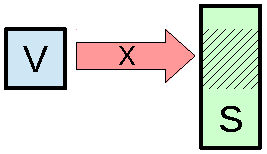
\includegraphics[width=3.5cm]{figures/Lens}
  \end{center}
  \vspace{-5ex}
  \caption{Visualisation of a simple lens}
  \label{fig:Lens}
  \end{figure}

  A lens $X : \view \lto \src$, for source type $\src$ and view type $\view$, identifies 
  $\view$ with a subregion of $\src$~\cite{Foster07,Foster09}, as illustrated in Figure~\ref{fig:Lens}. The arrow denotes 
  $X$ and the hatched area denotes the subregion $\view$ it characterises. Transformations on 
  $\view$ can be performed without affecting the parts of $\src$ outside the hatched area. The lens 
  signature consists of a pair of functions $\lget_X : \src \Rightarrow \view$ that extracts a view 
  from a source, and $\lput_X : \src \Rightarrow \view \Rightarrow \src$ that updates a view within 
  a given source.%
\end{isamarkuptext}\isamarkuptrue%
\isacommand{named{\isacharunderscore}theorems}\isamarkupfalse%
\ lens{\isacharunderscore}defs\isanewline
\isanewline
\isacommand{definition}\isamarkupfalse%
\ lens{\isacharunderscore}create\ {\isacharcolon}{\isacharcolon}\ {\isachardoublequoteopen}{\isacharparenleft}{\isacharprime}a\ {\isasymLongrightarrow}\ {\isacharprime}b{\isacharparenright}\ {\isasymRightarrow}\ {\isacharprime}a\ {\isasymRightarrow}\ {\isacharprime}b{\isachardoublequoteclose}\ {\isacharparenleft}{\isachardoublequoteopen}create{\isasymindex}{\isachardoublequoteclose}{\isacharparenright}\ \isakeyword{where}\isanewline
{\isacharbrackleft}lens{\isacharunderscore}defs{\isacharbrackright}{\isacharcolon}\ {\isachardoublequoteopen}create\isactrlbsub X\isactrlesub \ v\ {\isacharequal}\ put\isactrlbsub X\isactrlesub \ undefined\ v{\isachardoublequoteclose}%
\begin{isamarkuptext}%
Function $\lcreate_X~v$ creates an instance of the source type of $X$ by injecting $v$
  as the view, and leaving the remaining context arbitrary.%
\end{isamarkuptext}\isamarkuptrue%
%
\isamarkupsubsection{Weak lenses%
}
\isamarkuptrue%
%
\begin{isamarkuptext}%
Weak lenses are the least constrained class of lenses in our algebraic hierarchy. They
  simply require that the PutGet law~\cite{Foster09,Fischer2015} is satisfied, meaning that 
  $\lget$ is the inverse of $\lput$.%
\end{isamarkuptext}\isamarkuptrue%
\isacommand{locale}\isamarkupfalse%
\ weak{\isacharunderscore}lens\ {\isacharequal}\isanewline
\ \ \isakeyword{fixes}\ x\ {\isacharcolon}{\isacharcolon}\ {\isachardoublequoteopen}{\isacharprime}a\ {\isasymLongrightarrow}\ {\isacharprime}b{\isachardoublequoteclose}\ {\isacharparenleft}\isakeyword{structure}{\isacharparenright}\isanewline
\ \ \isakeyword{assumes}\ put{\isacharunderscore}get{\isacharcolon}\ {\isachardoublequoteopen}get\ {\isacharparenleft}put\ {\isasymsigma}\ v{\isacharparenright}\ {\isacharequal}\ v{\isachardoublequoteclose}\isanewline
\isakeyword{begin}\isanewline
\isanewline
\ \ \isacommand{lemma}\isamarkupfalse%
\ create{\isacharunderscore}get{\isacharcolon}\ {\isachardoublequoteopen}get\ {\isacharparenleft}create\ v{\isacharparenright}\ {\isacharequal}\ v{\isachardoublequoteclose}\isanewline
%
\isadelimproof
\ \ \ \ %
\endisadelimproof
%
\isatagproof
\isacommand{by}\isamarkupfalse%
\ {\isacharparenleft}simp\ add{\isacharcolon}\ lens{\isacharunderscore}create{\isacharunderscore}def\ put{\isacharunderscore}get{\isacharparenright}%
\endisatagproof
{\isafoldproof}%
%
\isadelimproof
\isanewline
%
\endisadelimproof
\isanewline
\ \ \isacommand{lemma}\isamarkupfalse%
\ create{\isacharunderscore}inj{\isacharcolon}\ {\isachardoublequoteopen}inj\ create{\isachardoublequoteclose}\isanewline
%
\isadelimproof
\ \ \ \ %
\endisadelimproof
%
\isatagproof
\isacommand{by}\isamarkupfalse%
\ {\isacharparenleft}metis\ create{\isacharunderscore}get\ injI{\isacharparenright}%
\endisatagproof
{\isafoldproof}%
%
\isadelimproof
\isanewline
%
\endisadelimproof
\isanewline
\ \ \isacommand{definition}\isamarkupfalse%
\ update\ {\isacharcolon}{\isacharcolon}\ {\isachardoublequoteopen}{\isacharparenleft}{\isacharprime}a\ {\isasymRightarrow}\ {\isacharprime}a{\isacharparenright}\ {\isasymRightarrow}\ {\isacharparenleft}{\isacharprime}b\ {\isasymRightarrow}\ {\isacharprime}b{\isacharparenright}{\isachardoublequoteclose}\ \isakeyword{where}\isanewline
\ \ {\isacharbrackleft}lens{\isacharunderscore}defs{\isacharbrackright}{\isacharcolon}\ {\isachardoublequoteopen}update\ f\ {\isasymsigma}\ {\isacharequal}\ put\ {\isasymsigma}\ {\isacharparenleft}f\ {\isacharparenleft}get\ {\isasymsigma}{\isacharparenright}{\isacharparenright}{\isachardoublequoteclose}\isanewline
\isanewline
\ \ \isacommand{lemma}\isamarkupfalse%
\ get{\isacharunderscore}update{\isacharcolon}\ {\isachardoublequoteopen}get\ {\isacharparenleft}update\ f\ {\isasymsigma}{\isacharparenright}\ {\isacharequal}\ f\ {\isacharparenleft}get\ {\isasymsigma}{\isacharparenright}{\isachardoublequoteclose}\isanewline
%
\isadelimproof
\ \ \ \ %
\endisadelimproof
%
\isatagproof
\isacommand{by}\isamarkupfalse%
\ {\isacharparenleft}simp\ add{\isacharcolon}\ put{\isacharunderscore}get\ update{\isacharunderscore}def{\isacharparenright}%
\endisatagproof
{\isafoldproof}%
%
\isadelimproof
\isanewline
%
\endisadelimproof
\isanewline
\ \ \isacommand{lemma}\isamarkupfalse%
\ view{\isacharunderscore}determination{\isacharcolon}\ {\isachardoublequoteopen}put\ {\isasymsigma}\ u\ {\isacharequal}\ put\ {\isasymrho}\ v\ {\isasymLongrightarrow}\ u\ {\isacharequal}\ v{\isachardoublequoteclose}\isanewline
%
\isadelimproof
\ \ \ \ %
\endisadelimproof
%
\isatagproof
\isacommand{by}\isamarkupfalse%
\ {\isacharparenleft}metis\ put{\isacharunderscore}get{\isacharparenright}%
\endisatagproof
{\isafoldproof}%
%
\isadelimproof
\isanewline
%
\endisadelimproof
\isanewline
\ \ \isacommand{lemma}\isamarkupfalse%
\ put{\isacharunderscore}inj{\isacharcolon}\ {\isachardoublequoteopen}inj\ {\isacharparenleft}put\ {\isasymsigma}{\isacharparenright}{\isachardoublequoteclose}\isanewline
%
\isadelimproof
\ \ \ \ %
\endisadelimproof
%
\isatagproof
\isacommand{by}\isamarkupfalse%
\ {\isacharparenleft}simp\ add{\isacharcolon}\ injI\ view{\isacharunderscore}determination{\isacharparenright}%
\endisatagproof
{\isafoldproof}%
%
\isadelimproof
\isanewline
%
\endisadelimproof
\isacommand{end}\isamarkupfalse%
\isanewline
\isanewline
\isacommand{declare}\isamarkupfalse%
\ weak{\isacharunderscore}lens{\isachardot}put{\isacharunderscore}get\ {\isacharbrackleft}simp{\isacharbrackright}\isanewline
\isacommand{declare}\isamarkupfalse%
\ weak{\isacharunderscore}lens{\isachardot}create{\isacharunderscore}get\ {\isacharbrackleft}simp{\isacharbrackright}%
\isamarkupsubsection{Well-behaved lenses%
}
\isamarkuptrue%
%
\begin{isamarkuptext}%
Well-behaved lenses add to weak lenses that requirement that the GetPut law~\cite{Foster09,Fischer2015} 
  is satisfied, meaning that $\lput$ is the inverse of $\lget$.%
\end{isamarkuptext}\isamarkuptrue%
\isacommand{locale}\isamarkupfalse%
\ wb{\isacharunderscore}lens\ {\isacharequal}\ weak{\isacharunderscore}lens\ {\isacharplus}\isanewline
\ \ \isakeyword{assumes}\ get{\isacharunderscore}put{\isacharcolon}\ {\isachardoublequoteopen}put\ {\isasymsigma}\ {\isacharparenleft}get\ {\isasymsigma}{\isacharparenright}\ {\isacharequal}\ {\isasymsigma}{\isachardoublequoteclose}\isanewline
\isakeyword{begin}\isanewline
\isanewline
\ \ \isacommand{lemma}\isamarkupfalse%
\ put{\isacharunderscore}twice{\isacharcolon}\ {\isachardoublequoteopen}put\ {\isacharparenleft}put\ {\isasymsigma}\ v{\isacharparenright}\ v\ {\isacharequal}\ put\ {\isasymsigma}\ v{\isachardoublequoteclose}\isanewline
%
\isadelimproof
\ \ \ \ %
\endisadelimproof
%
\isatagproof
\isacommand{by}\isamarkupfalse%
\ {\isacharparenleft}metis\ get{\isacharunderscore}put\ put{\isacharunderscore}get{\isacharparenright}%
\endisatagproof
{\isafoldproof}%
%
\isadelimproof
\isanewline
%
\endisadelimproof
\isanewline
\ \ \isacommand{lemma}\isamarkupfalse%
\ put{\isacharunderscore}surjectivity{\isacharcolon}\ {\isachardoublequoteopen}{\isasymexists}\ {\isasymrho}\ v{\isachardot}\ put\ {\isasymrho}\ v\ {\isacharequal}\ {\isasymsigma}{\isachardoublequoteclose}\isanewline
%
\isadelimproof
\ \ \ \ %
\endisadelimproof
%
\isatagproof
\isacommand{using}\isamarkupfalse%
\ get{\isacharunderscore}put\ \isacommand{by}\isamarkupfalse%
\ blast%
\endisatagproof
{\isafoldproof}%
%
\isadelimproof
\isanewline
%
\endisadelimproof
\isanewline
\ \ \isacommand{lemma}\isamarkupfalse%
\ source{\isacharunderscore}stability{\isacharcolon}\ {\isachardoublequoteopen}{\isasymexists}\ v{\isachardot}\ put\ {\isasymsigma}\ v\ {\isacharequal}\ {\isasymsigma}{\isachardoublequoteclose}\isanewline
%
\isadelimproof
\ \ \ \ %
\endisadelimproof
%
\isatagproof
\isacommand{using}\isamarkupfalse%
\ get{\isacharunderscore}put\ \isacommand{by}\isamarkupfalse%
\ auto%
\endisatagproof
{\isafoldproof}%
%
\isadelimproof
\isanewline
%
\endisadelimproof
\isanewline
\isacommand{end}\isamarkupfalse%
\isanewline
\isanewline
\isacommand{declare}\isamarkupfalse%
\ wb{\isacharunderscore}lens{\isachardot}get{\isacharunderscore}put\ {\isacharbrackleft}simp{\isacharbrackright}\isanewline
\isanewline
\isacommand{lemma}\isamarkupfalse%
\ wb{\isacharunderscore}lens{\isacharunderscore}weak\ {\isacharbrackleft}simp{\isacharbrackright}{\isacharcolon}\ {\isachardoublequoteopen}wb{\isacharunderscore}lens\ x\ {\isasymLongrightarrow}\ weak{\isacharunderscore}lens\ x{\isachardoublequoteclose}\isanewline
%
\isadelimproof
\ \ %
\endisadelimproof
%
\isatagproof
\isacommand{by}\isamarkupfalse%
\ {\isacharparenleft}simp{\isacharunderscore}all\ add{\isacharcolon}\ wb{\isacharunderscore}lens{\isacharunderscore}def{\isacharparenright}%
\endisatagproof
{\isafoldproof}%
%
\isadelimproof
%
\endisadelimproof
%
\isamarkupsubsection{Mainly well-behaved lenses%
}
\isamarkuptrue%
%
\begin{isamarkuptext}%
Mainly well-behaved lenses extend weak lenses with the PutPut law that shows how one put
  override a previous one.%
\end{isamarkuptext}\isamarkuptrue%
\isacommand{locale}\isamarkupfalse%
\ mwb{\isacharunderscore}lens\ {\isacharequal}\ weak{\isacharunderscore}lens\ {\isacharplus}\isanewline
\ \ \isakeyword{assumes}\ put{\isacharunderscore}put{\isacharcolon}\ {\isachardoublequoteopen}put\ {\isacharparenleft}put\ {\isasymsigma}\ v{\isacharparenright}\ u\ {\isacharequal}\ put\ {\isasymsigma}\ u{\isachardoublequoteclose}\isanewline
\isakeyword{begin}\isanewline
\isanewline
\ \ \isacommand{lemma}\isamarkupfalse%
\ update{\isacharunderscore}comp{\isacharcolon}\ {\isachardoublequoteopen}update\ f\ {\isacharparenleft}update\ g\ {\isasymsigma}{\isacharparenright}\ {\isacharequal}\ update\ {\isacharparenleft}f\ {\isasymcirc}\ g{\isacharparenright}\ {\isasymsigma}{\isachardoublequoteclose}\isanewline
%
\isadelimproof
\ \ \ \ %
\endisadelimproof
%
\isatagproof
\isacommand{by}\isamarkupfalse%
\ {\isacharparenleft}simp\ add{\isacharcolon}\ put{\isacharunderscore}get\ put{\isacharunderscore}put\ update{\isacharunderscore}def{\isacharparenright}%
\endisatagproof
{\isafoldproof}%
%
\isadelimproof
\isanewline
%
\endisadelimproof
\isanewline
\isacommand{end}\isamarkupfalse%
\isanewline
\isanewline
\isacommand{declare}\isamarkupfalse%
\ mwb{\isacharunderscore}lens{\isachardot}put{\isacharunderscore}put\ {\isacharbrackleft}simp{\isacharbrackright}\isanewline
\isanewline
\isacommand{lemma}\isamarkupfalse%
\ mwb{\isacharunderscore}lens{\isacharunderscore}weak\ {\isacharbrackleft}simp{\isacharbrackright}{\isacharcolon}\isanewline
\ \ {\isachardoublequoteopen}mwb{\isacharunderscore}lens\ x\ {\isasymLongrightarrow}\ weak{\isacharunderscore}lens\ x{\isachardoublequoteclose}\isanewline
%
\isadelimproof
\ \ %
\endisadelimproof
%
\isatagproof
\isacommand{by}\isamarkupfalse%
\ {\isacharparenleft}simp\ add{\isacharcolon}\ mwb{\isacharunderscore}lens{\isacharunderscore}def{\isacharparenright}%
\endisatagproof
{\isafoldproof}%
%
\isadelimproof
%
\endisadelimproof
%
\isamarkupsubsection{Very well-behaved lenses%
}
\isamarkuptrue%
%
\begin{isamarkuptext}%
Very well-behaved lenses combine all three laws, as in the literature~\cite{Foster09,Fischer2015}.%
\end{isamarkuptext}\isamarkuptrue%
\isacommand{locale}\isamarkupfalse%
\ vwb{\isacharunderscore}lens\ {\isacharequal}\ wb{\isacharunderscore}lens\ {\isacharplus}\ mwb{\isacharunderscore}lens\isanewline
\isakeyword{begin}\isanewline
\isanewline
\ \ \isacommand{lemma}\isamarkupfalse%
\ source{\isacharunderscore}determination{\isacharcolon}{\isachardoublequoteopen}get\ {\isasymsigma}\ {\isacharequal}\ get\ {\isasymrho}\ {\isasymLongrightarrow}\ put\ {\isasymsigma}\ v\ {\isacharequal}\ put\ {\isasymrho}\ v\ {\isasymLongrightarrow}\ {\isasymsigma}\ {\isacharequal}\ {\isasymrho}{\isachardoublequoteclose}\isanewline
%
\isadelimproof
\ \ \ \ %
\endisadelimproof
%
\isatagproof
\isacommand{by}\isamarkupfalse%
\ {\isacharparenleft}metis\ get{\isacharunderscore}put\ put{\isacharunderscore}put{\isacharparenright}%
\endisatagproof
{\isafoldproof}%
%
\isadelimproof
\isanewline
%
\endisadelimproof
\isanewline
\ \isacommand{lemma}\isamarkupfalse%
\ put{\isacharunderscore}eq{\isacharcolon}\isanewline
\ \ \ {\isachardoublequoteopen}{\isasymlbrakk}\ get\ {\isasymsigma}\ {\isacharequal}\ k{\isacharsemicolon}\ put\ {\isasymsigma}\ u\ {\isacharequal}\ put\ {\isasymrho}\ v\ {\isasymrbrakk}\ {\isasymLongrightarrow}\ put\ {\isasymrho}\ k\ {\isacharequal}\ {\isasymsigma}{\isachardoublequoteclose}\isanewline
%
\isadelimproof
\ \ \ %
\endisadelimproof
%
\isatagproof
\isacommand{by}\isamarkupfalse%
\ {\isacharparenleft}metis\ get{\isacharunderscore}put\ put{\isacharunderscore}put{\isacharparenright}%
\endisatagproof
{\isafoldproof}%
%
\isadelimproof
\isanewline
%
\endisadelimproof
\isanewline
\isacommand{end}\isamarkupfalse%
\isanewline
\isanewline
\isacommand{lemma}\isamarkupfalse%
\ vwb{\isacharunderscore}lens{\isacharunderscore}wb\ {\isacharbrackleft}simp{\isacharbrackright}{\isacharcolon}\ {\isachardoublequoteopen}vwb{\isacharunderscore}lens\ x\ {\isasymLongrightarrow}\ wb{\isacharunderscore}lens\ x{\isachardoublequoteclose}\isanewline
%
\isadelimproof
\ \ %
\endisadelimproof
%
\isatagproof
\isacommand{by}\isamarkupfalse%
\ {\isacharparenleft}simp{\isacharunderscore}all\ add{\isacharcolon}\ vwb{\isacharunderscore}lens{\isacharunderscore}def{\isacharparenright}%
\endisatagproof
{\isafoldproof}%
%
\isadelimproof
\isanewline
%
\endisadelimproof
\isanewline
\isacommand{lemma}\isamarkupfalse%
\ vwb{\isacharunderscore}lens{\isacharunderscore}mwb\ {\isacharbrackleft}simp{\isacharbrackright}{\isacharcolon}\ {\isachardoublequoteopen}vwb{\isacharunderscore}lens\ x\ {\isasymLongrightarrow}\ mwb{\isacharunderscore}lens\ x{\isachardoublequoteclose}\isanewline
%
\isadelimproof
\ \ %
\endisadelimproof
%
\isatagproof
\isacommand{by}\isamarkupfalse%
\ {\isacharparenleft}simp{\isacharunderscore}all\ add{\isacharcolon}\ vwb{\isacharunderscore}lens{\isacharunderscore}def{\isacharparenright}%
\endisatagproof
{\isafoldproof}%
%
\isadelimproof
%
\endisadelimproof
%
\isamarkupsubsection{Ineffectual lenses%
}
\isamarkuptrue%
%
\begin{isamarkuptext}%
Ineffectual lenses can have no effect on the view type -- application of the $\lput$ function
  always yields the same source. They are trivially very well-behaved lenses.%
\end{isamarkuptext}\isamarkuptrue%
\isacommand{locale}\isamarkupfalse%
\ ief{\isacharunderscore}lens\ {\isacharequal}\ weak{\isacharunderscore}lens\ {\isacharplus}\isanewline
\ \ \isakeyword{assumes}\ put{\isacharunderscore}inef{\isacharcolon}\ {\isachardoublequoteopen}put\ {\isasymsigma}\ v\ {\isacharequal}\ {\isasymsigma}{\isachardoublequoteclose}\isanewline
\isakeyword{begin}\isanewline
\isanewline
\isacommand{sublocale}\isamarkupfalse%
\ vwb{\isacharunderscore}lens\isanewline
%
\isadelimproof
%
\endisadelimproof
%
\isatagproof
\isacommand{proof}\isamarkupfalse%
\isanewline
\ \ \isacommand{fix}\isamarkupfalse%
\ {\isasymsigma}\ v\ u\isanewline
\ \ \isacommand{show}\isamarkupfalse%
\ {\isachardoublequoteopen}put\ {\isasymsigma}\ {\isacharparenleft}get\ {\isasymsigma}{\isacharparenright}\ {\isacharequal}\ {\isasymsigma}{\isachardoublequoteclose}\isanewline
\ \ \ \ \isacommand{by}\isamarkupfalse%
\ {\isacharparenleft}simp\ add{\isacharcolon}\ put{\isacharunderscore}inef{\isacharparenright}\isanewline
\ \ \isacommand{show}\isamarkupfalse%
\ {\isachardoublequoteopen}put\ {\isacharparenleft}put\ {\isasymsigma}\ v{\isacharparenright}\ u\ {\isacharequal}\ put\ {\isasymsigma}\ u{\isachardoublequoteclose}\isanewline
\ \ \ \ \isacommand{by}\isamarkupfalse%
\ {\isacharparenleft}simp\ add{\isacharcolon}\ put{\isacharunderscore}inef{\isacharparenright}\isanewline
\isacommand{qed}\isamarkupfalse%
%
\endisatagproof
{\isafoldproof}%
%
\isadelimproof
\isanewline
%
\endisadelimproof
\isanewline
\isacommand{lemma}\isamarkupfalse%
\ ineffectual{\isacharunderscore}const{\isacharunderscore}get{\isacharcolon}\isanewline
\ \ {\isachardoublequoteopen}{\isasymexists}\ v{\isachardot}\ \ {\isasymforall}\ {\isasymsigma}{\isachardot}\ get\ {\isasymsigma}\ {\isacharequal}\ v{\isachardoublequoteclose}\isanewline
%
\isadelimproof
\ \ %
\endisadelimproof
%
\isatagproof
\isacommand{by}\isamarkupfalse%
\ {\isacharparenleft}metis\ create{\isacharunderscore}get\ lens{\isacharunderscore}create{\isacharunderscore}def\ put{\isacharunderscore}inef{\isacharparenright}%
\endisatagproof
{\isafoldproof}%
%
\isadelimproof
\isanewline
%
\endisadelimproof
\isanewline
\isacommand{end}\isamarkupfalse%
\isanewline
\isanewline
\isacommand{abbreviation}\isamarkupfalse%
\ {\isachardoublequoteopen}eff{\isacharunderscore}lens\ X\ {\isasymequiv}\ {\isacharparenleft}weak{\isacharunderscore}lens\ X\ {\isasymand}\ {\isacharparenleft}{\isasymnot}\ ief{\isacharunderscore}lens\ X{\isacharparenright}{\isacharparenright}{\isachardoublequoteclose}%
\isamarkupsubsection{Bijective lenses%
}
\isamarkuptrue%
%
\begin{isamarkuptext}%
Bijective lenses characterise the situation where the source and view type are equivalent:
  in other words the view type full characterises the whole source type. This is specified using
  the strong GetPut law~\cite{Foster09,Fischer2015}.%
\end{isamarkuptext}\isamarkuptrue%
\isacommand{locale}\isamarkupfalse%
\ bij{\isacharunderscore}lens\ {\isacharequal}\ weak{\isacharunderscore}lens\ {\isacharplus}\isanewline
\ \ \isakeyword{assumes}\ strong{\isacharunderscore}get{\isacharunderscore}put{\isacharcolon}\ {\isachardoublequoteopen}put\ {\isasymsigma}\ {\isacharparenleft}get\ {\isasymrho}{\isacharparenright}\ {\isacharequal}\ {\isasymrho}{\isachardoublequoteclose}\isanewline
\isakeyword{begin}\isanewline
\isanewline
\isacommand{sublocale}\isamarkupfalse%
\ vwb{\isacharunderscore}lens\isanewline
%
\isadelimproof
%
\endisadelimproof
%
\isatagproof
\isacommand{proof}\isamarkupfalse%
\isanewline
\ \ \isacommand{fix}\isamarkupfalse%
\ {\isasymsigma}\ v\ u\isanewline
\ \ \isacommand{show}\isamarkupfalse%
\ {\isachardoublequoteopen}put\ {\isasymsigma}\ {\isacharparenleft}get\ {\isasymsigma}{\isacharparenright}\ {\isacharequal}\ {\isasymsigma}{\isachardoublequoteclose}\isanewline
\ \ \ \ \isacommand{by}\isamarkupfalse%
\ {\isacharparenleft}simp\ add{\isacharcolon}\ strong{\isacharunderscore}get{\isacharunderscore}put{\isacharparenright}\isanewline
\ \ \isacommand{show}\isamarkupfalse%
\ {\isachardoublequoteopen}put\ {\isacharparenleft}put\ {\isasymsigma}\ v{\isacharparenright}\ u\ {\isacharequal}\ put\ {\isasymsigma}\ u{\isachardoublequoteclose}\isanewline
\ \ \ \ \isacommand{by}\isamarkupfalse%
\ {\isacharparenleft}metis\ put{\isacharunderscore}get\ strong{\isacharunderscore}get{\isacharunderscore}put{\isacharparenright}\isanewline
\isacommand{qed}\isamarkupfalse%
%
\endisatagproof
{\isafoldproof}%
%
\isadelimproof
\isanewline
%
\endisadelimproof
\isanewline
\ \ \isacommand{lemma}\isamarkupfalse%
\ put{\isacharunderscore}surj{\isacharcolon}\ {\isachardoublequoteopen}surj\ {\isacharparenleft}put\ {\isasymsigma}{\isacharparenright}{\isachardoublequoteclose}\isanewline
%
\isadelimproof
\ \ \ \ %
\endisadelimproof
%
\isatagproof
\isacommand{by}\isamarkupfalse%
\ {\isacharparenleft}metis\ strong{\isacharunderscore}get{\isacharunderscore}put\ surj{\isacharunderscore}def{\isacharparenright}%
\endisatagproof
{\isafoldproof}%
%
\isadelimproof
\isanewline
%
\endisadelimproof
\isanewline
\ \ \isacommand{lemma}\isamarkupfalse%
\ put{\isacharunderscore}bij{\isacharcolon}\ {\isachardoublequoteopen}bij\ {\isacharparenleft}put\ {\isasymsigma}{\isacharparenright}{\isachardoublequoteclose}\isanewline
%
\isadelimproof
\ \ \ \ %
\endisadelimproof
%
\isatagproof
\isacommand{by}\isamarkupfalse%
\ {\isacharparenleft}simp\ add{\isacharcolon}\ bijI\ put{\isacharunderscore}inj\ put{\isacharunderscore}surj{\isacharparenright}%
\endisatagproof
{\isafoldproof}%
%
\isadelimproof
\isanewline
%
\endisadelimproof
\isanewline
\ \ \isacommand{lemma}\isamarkupfalse%
\ put{\isacharunderscore}is{\isacharunderscore}create{\isacharcolon}\ {\isachardoublequoteopen}put\ {\isasymsigma}\ v\ {\isacharequal}\ create\ v{\isachardoublequoteclose}\isanewline
%
\isadelimproof
\ \ \ \ %
\endisadelimproof
%
\isatagproof
\isacommand{by}\isamarkupfalse%
\ {\isacharparenleft}metis\ create{\isacharunderscore}get\ strong{\isacharunderscore}get{\isacharunderscore}put{\isacharparenright}%
\endisatagproof
{\isafoldproof}%
%
\isadelimproof
\isanewline
%
\endisadelimproof
\isanewline
\ \ \isacommand{lemma}\isamarkupfalse%
\ get{\isacharunderscore}create{\isacharcolon}\ {\isachardoublequoteopen}create\ {\isacharparenleft}get\ {\isasymsigma}{\isacharparenright}\ {\isacharequal}\ {\isasymsigma}{\isachardoublequoteclose}\isanewline
%
\isadelimproof
\ \ \ \ %
\endisadelimproof
%
\isatagproof
\isacommand{by}\isamarkupfalse%
\ {\isacharparenleft}metis\ put{\isacharunderscore}get\ put{\isacharunderscore}is{\isacharunderscore}create\ source{\isacharunderscore}stability{\isacharparenright}%
\endisatagproof
{\isafoldproof}%
%
\isadelimproof
\isanewline
%
\endisadelimproof
\isanewline
\isacommand{end}\isamarkupfalse%
\isanewline
\isanewline
\isacommand{declare}\isamarkupfalse%
\ bij{\isacharunderscore}lens{\isachardot}strong{\isacharunderscore}get{\isacharunderscore}put\ {\isacharbrackleft}simp{\isacharbrackright}\isanewline
\isacommand{declare}\isamarkupfalse%
\ bij{\isacharunderscore}lens{\isachardot}get{\isacharunderscore}create\ {\isacharbrackleft}simp{\isacharbrackright}\isanewline
\isanewline
\isacommand{lemma}\isamarkupfalse%
\ bij{\isacharunderscore}lens{\isacharunderscore}weak\ {\isacharbrackleft}simp{\isacharbrackright}{\isacharcolon}\isanewline
\ \ {\isachardoublequoteopen}bij{\isacharunderscore}lens\ x\ {\isasymLongrightarrow}\ weak{\isacharunderscore}lens\ x{\isachardoublequoteclose}\isanewline
%
\isadelimproof
\ \ %
\endisadelimproof
%
\isatagproof
\isacommand{by}\isamarkupfalse%
\ {\isacharparenleft}simp{\isacharunderscore}all\ add{\isacharcolon}\ bij{\isacharunderscore}lens{\isacharunderscore}def{\isacharparenright}%
\endisatagproof
{\isafoldproof}%
%
\isadelimproof
\isanewline
%
\endisadelimproof
\isanewline
\isacommand{lemma}\isamarkupfalse%
\ bij{\isacharunderscore}lens{\isacharunderscore}vwb\ {\isacharbrackleft}simp{\isacharbrackright}{\isacharcolon}\ {\isachardoublequoteopen}bij{\isacharunderscore}lens\ x\ {\isasymLongrightarrow}\ vwb{\isacharunderscore}lens\ x{\isachardoublequoteclose}\isanewline
%
\isadelimproof
\ \ %
\endisadelimproof
%
\isatagproof
\isacommand{by}\isamarkupfalse%
\ {\isacharparenleft}unfold{\isacharunderscore}locales{\isacharcomma}\ simp{\isacharunderscore}all\ add{\isacharcolon}\ bij{\isacharunderscore}lens{\isachardot}put{\isacharunderscore}is{\isacharunderscore}create{\isacharparenright}%
\endisatagproof
{\isafoldproof}%
%
\isadelimproof
%
\endisadelimproof
%
\isamarkupsubsection{Lens independence%
}
\isamarkuptrue%
%
\begin{isamarkuptext}%
Lens independence shows when two lenses $X$ and $Y$ characterise disjoint regions of the 
  source type. We specify this by requiring that the $\lput$ functions of the two lenses commute,
  and that the $\lget$ function of each lens is unaffected by application of $\lput$ from the
  corresponding lens.%
\end{isamarkuptext}\isamarkuptrue%
\isacommand{locale}\isamarkupfalse%
\ lens{\isacharunderscore}indep\ {\isacharequal}\isanewline
\ \ \isakeyword{fixes}\ X\ {\isacharcolon}{\isacharcolon}\ {\isachardoublequoteopen}{\isacharprime}a\ {\isasymLongrightarrow}\ {\isacharprime}c{\isachardoublequoteclose}\ \isakeyword{and}\ Y\ {\isacharcolon}{\isacharcolon}\ {\isachardoublequoteopen}{\isacharprime}b\ {\isasymLongrightarrow}\ {\isacharprime}c{\isachardoublequoteclose}\isanewline
\ \ \isakeyword{assumes}\ lens{\isacharunderscore}put{\isacharunderscore}comm{\isacharcolon}\ {\isachardoublequoteopen}lens{\isacharunderscore}put\ X\ {\isacharparenleft}lens{\isacharunderscore}put\ Y\ {\isasymsigma}\ v{\isacharparenright}\ u\ {\isacharequal}\ lens{\isacharunderscore}put\ Y\ {\isacharparenleft}lens{\isacharunderscore}put\ X\ {\isasymsigma}\ u{\isacharparenright}\ v{\isachardoublequoteclose}\isanewline
\ \ \isakeyword{and}\ lens{\isacharunderscore}put{\isacharunderscore}irr{\isadigit{1}}{\isacharcolon}\ {\isachardoublequoteopen}lens{\isacharunderscore}get\ X\ {\isacharparenleft}lens{\isacharunderscore}put\ Y\ {\isasymsigma}\ v{\isacharparenright}\ {\isacharequal}\ lens{\isacharunderscore}get\ X\ {\isasymsigma}{\isachardoublequoteclose}\isanewline
\ \ \isakeyword{and}\ lens{\isacharunderscore}put{\isacharunderscore}irr{\isadigit{2}}{\isacharcolon}\ {\isachardoublequoteopen}lens{\isacharunderscore}get\ Y\ {\isacharparenleft}lens{\isacharunderscore}put\ X\ {\isasymsigma}\ u{\isacharparenright}\ {\isacharequal}\ lens{\isacharunderscore}get\ Y\ {\isasymsigma}{\isachardoublequoteclose}\isanewline
\isanewline
\isacommand{notation}\isamarkupfalse%
\ lens{\isacharunderscore}indep\ {\isacharparenleft}\isakeyword{infix}\ {\isachardoublequoteopen}{\isasymbowtie}{\isachardoublequoteclose}\ {\isadigit{5}}{\isadigit{0}}{\isacharparenright}\isanewline
\isanewline
\isacommand{lemma}\isamarkupfalse%
\ lens{\isacharunderscore}indepI{\isacharcolon}\isanewline
\ \ {\isachardoublequoteopen}{\isasymlbrakk}\ {\isasymAnd}\ u\ v\ {\isasymsigma}{\isachardot}\ lens{\isacharunderscore}put\ x\ {\isacharparenleft}lens{\isacharunderscore}put\ y\ {\isasymsigma}\ v{\isacharparenright}\ u\ {\isacharequal}\ lens{\isacharunderscore}put\ y\ {\isacharparenleft}lens{\isacharunderscore}put\ x\ {\isasymsigma}\ u{\isacharparenright}\ v{\isacharsemicolon}\isanewline
\ \ \ \ \ {\isasymAnd}\ v\ {\isasymsigma}{\isachardot}\ lens{\isacharunderscore}get\ x\ {\isacharparenleft}lens{\isacharunderscore}put\ y\ {\isasymsigma}\ v{\isacharparenright}\ {\isacharequal}\ lens{\isacharunderscore}get\ x\ {\isasymsigma}{\isacharsemicolon}\isanewline
\ \ \ \ \ {\isasymAnd}\ u\ {\isasymsigma}{\isachardot}\ lens{\isacharunderscore}get\ y\ {\isacharparenleft}lens{\isacharunderscore}put\ x\ {\isasymsigma}\ u{\isacharparenright}\ {\isacharequal}\ lens{\isacharunderscore}get\ y\ {\isasymsigma}\ {\isasymrbrakk}\ {\isasymLongrightarrow}\ x\ {\isasymbowtie}\ y{\isachardoublequoteclose}\isanewline
%
\isadelimproof
\ \ %
\endisadelimproof
%
\isatagproof
\isacommand{by}\isamarkupfalse%
\ {\isacharparenleft}simp\ add{\isacharcolon}\ lens{\isacharunderscore}indep{\isacharunderscore}def{\isacharparenright}%
\endisatagproof
{\isafoldproof}%
%
\isadelimproof
%
\endisadelimproof
%
\begin{isamarkuptext}%
Independence is symmetric.%
\end{isamarkuptext}\isamarkuptrue%
\isacommand{lemma}\isamarkupfalse%
\ lens{\isacharunderscore}indep{\isacharunderscore}sym{\isacharcolon}\ \ {\isachardoublequoteopen}x\ {\isasymbowtie}\ y\ {\isasymLongrightarrow}\ y\ {\isasymbowtie}\ x{\isachardoublequoteclose}\isanewline
%
\isadelimproof
\ \ %
\endisadelimproof
%
\isatagproof
\isacommand{by}\isamarkupfalse%
\ {\isacharparenleft}simp\ add{\isacharcolon}\ lens{\isacharunderscore}indep{\isacharunderscore}def{\isacharparenright}%
\endisatagproof
{\isafoldproof}%
%
\isadelimproof
\isanewline
%
\endisadelimproof
\ \ \ \ \isanewline
\isacommand{lemma}\isamarkupfalse%
\ lens{\isacharunderscore}indep{\isacharunderscore}comm{\isacharcolon}\isanewline
\ \ {\isachardoublequoteopen}x\ {\isasymbowtie}\ y\ {\isasymLongrightarrow}\ lens{\isacharunderscore}put\ x\ {\isacharparenleft}lens{\isacharunderscore}put\ y\ {\isasymsigma}\ v{\isacharparenright}\ u\ {\isacharequal}\ lens{\isacharunderscore}put\ y\ {\isacharparenleft}lens{\isacharunderscore}put\ x\ {\isasymsigma}\ u{\isacharparenright}\ v{\isachardoublequoteclose}\isanewline
%
\isadelimproof
\ \ %
\endisadelimproof
%
\isatagproof
\isacommand{by}\isamarkupfalse%
\ {\isacharparenleft}simp\ add{\isacharcolon}\ lens{\isacharunderscore}indep{\isacharunderscore}def{\isacharparenright}%
\endisatagproof
{\isafoldproof}%
%
\isadelimproof
\isanewline
%
\endisadelimproof
\isanewline
\isacommand{lemma}\isamarkupfalse%
\ lens{\isacharunderscore}indep{\isacharunderscore}get\ {\isacharbrackleft}simp{\isacharbrackright}{\isacharcolon}\isanewline
\ \ \isakeyword{assumes}\ {\isachardoublequoteopen}x\ {\isasymbowtie}\ y{\isachardoublequoteclose}\isanewline
\ \ \isakeyword{shows}\ {\isachardoublequoteopen}lens{\isacharunderscore}get\ x\ {\isacharparenleft}lens{\isacharunderscore}put\ y\ {\isasymsigma}\ v{\isacharparenright}\ {\isacharequal}\ lens{\isacharunderscore}get\ x\ {\isasymsigma}{\isachardoublequoteclose}\isanewline
%
\isadelimproof
\ \ %
\endisadelimproof
%
\isatagproof
\isacommand{using}\isamarkupfalse%
\ assms\ lens{\isacharunderscore}indep{\isacharunderscore}def\ \isacommand{by}\isamarkupfalse%
\ fastforce%
\endisatagproof
{\isafoldproof}%
%
\isadelimproof
\isanewline
%
\endisadelimproof
%
\isadelimtheory
\isanewline
%
\endisadelimtheory
%
\isatagtheory
\isacommand{end}\isamarkupfalse%
%
\endisatagtheory
{\isafoldtheory}%
%
\isadelimtheory
%
\endisadelimtheory
%
\end{isabellebody}%
%%% Local Variables:
%%% mode: latex
%%% TeX-master: "root"
%%% End:


%
\begin{isabellebody}%
\setisabellecontext{Lens{\isacharunderscore}Algebra}%
%
\isamarkupsection{Lens algebraic operators%
}
\isamarkuptrue%
%
\isadelimtheory
%
\endisadelimtheory
%
\isatagtheory
\isacommand{theory}\isamarkupfalse%
\ Lens{\isacharunderscore}Algebra\isanewline
\isakeyword{imports}\ Lens{\isacharunderscore}Laws\isanewline
\isakeyword{begin}%
\endisatagtheory
{\isafoldtheory}%
%
\isadelimtheory
%
\endisadelimtheory
%
\isamarkupsubsection{Lens composition, plus, unit, and identity%
}
\isamarkuptrue%
%
\begin{isamarkuptext}%
We introduce the algebraic lens operators; for more information please see our paper~\cite{Foster16a}.
      Lens composition constructs a lens by composing the source of one lens with the view of another.%
\end{isamarkuptext}\isamarkuptrue%
\isacommand{definition}\isamarkupfalse%
\ lens{\isacharunderscore}comp\ {\isacharcolon}{\isacharcolon}\ {\isachardoublequoteopen}{\isacharparenleft}{\isacharprime}a\ {\isasymLongrightarrow}\ {\isacharprime}b{\isacharparenright}\ {\isasymRightarrow}\ {\isacharparenleft}{\isacharprime}b\ {\isasymLongrightarrow}\ {\isacharprime}c{\isacharparenright}\ {\isasymRightarrow}\ {\isacharparenleft}{\isacharprime}a\ {\isasymLongrightarrow}\ {\isacharprime}c{\isacharparenright}{\isachardoublequoteclose}\ {\isacharparenleft}\isakeyword{infixr}\ {\isachardoublequoteopen}{\isacharsemicolon}\isactrlsub L{\isachardoublequoteclose}\ {\isadigit{8}}{\isadigit{0}}{\isacharparenright}\ \isakeyword{where}\isanewline
{\isacharbrackleft}lens{\isacharunderscore}defs{\isacharbrackright}{\isacharcolon}\ {\isachardoublequoteopen}lens{\isacharunderscore}comp\ Y\ X\ {\isacharequal}\ {\isasymlparr}\ lens{\isacharunderscore}get\ {\isacharequal}\ lens{\isacharunderscore}get\ Y\ {\isasymcirc}\ lens{\isacharunderscore}get\ X\isanewline
\ \ \ \ \ \ \ \ \ \ \ \ \ \ \ \ \ \ \ \ \ \ \ \ \ \ \ \ \ \ {\isacharcomma}\ lens{\isacharunderscore}put\ {\isacharequal}\ {\isacharparenleft}{\isasymlambda}\ {\isasymsigma}\ v{\isachardot}\ lens{\isacharunderscore}put\ X\ {\isasymsigma}\ {\isacharparenleft}lens{\isacharunderscore}put\ Y\ {\isacharparenleft}lens{\isacharunderscore}get\ X\ {\isasymsigma}{\isacharparenright}\ v{\isacharparenright}{\isacharparenright}\ {\isasymrparr}{\isachardoublequoteclose}%
\begin{isamarkuptext}%
Lens plus parallel composes two indepedent lenses, resulting in a lens whose view is the 
  product of the two underlying lens views.%
\end{isamarkuptext}\isamarkuptrue%
\isacommand{definition}\isamarkupfalse%
\ lens{\isacharunderscore}plus\ {\isacharcolon}{\isacharcolon}\ {\isachardoublequoteopen}{\isacharparenleft}{\isacharprime}a\ {\isasymLongrightarrow}\ {\isacharprime}c{\isacharparenright}\ {\isasymRightarrow}\ {\isacharparenleft}{\isacharprime}b\ {\isasymLongrightarrow}\ {\isacharprime}c{\isacharparenright}\ {\isasymRightarrow}\ {\isacharprime}a\ {\isasymtimes}\ {\isacharprime}b\ {\isasymLongrightarrow}\ {\isacharprime}c{\isachardoublequoteclose}\ {\isacharparenleft}\isakeyword{infixr}\ {\isachardoublequoteopen}{\isacharplus}\isactrlsub L{\isachardoublequoteclose}\ {\isadigit{7}}{\isadigit{5}}{\isacharparenright}\ \isakeyword{where}\isanewline
{\isacharbrackleft}lens{\isacharunderscore}defs{\isacharbrackright}{\isacharcolon}\ {\isachardoublequoteopen}X\ {\isacharplus}\isactrlsub L\ Y\ {\isacharequal}\ {\isasymlparr}\ lens{\isacharunderscore}get\ {\isacharequal}\ {\isacharparenleft}{\isasymlambda}\ {\isasymsigma}{\isachardot}\ {\isacharparenleft}lens{\isacharunderscore}get\ X\ {\isasymsigma}{\isacharcomma}\ lens{\isacharunderscore}get\ Y\ {\isasymsigma}{\isacharparenright}{\isacharparenright}\isanewline
\ \ \ \ \ \ \ \ \ \ \ \ \ \ \ \ \ \ \ \ \ \ \ {\isacharcomma}\ lens{\isacharunderscore}put\ {\isacharequal}\ {\isacharparenleft}{\isasymlambda}\ {\isasymsigma}\ {\isacharparenleft}u{\isacharcomma}\ v{\isacharparenright}{\isachardot}\ lens{\isacharunderscore}put\ X\ {\isacharparenleft}lens{\isacharunderscore}put\ Y\ {\isasymsigma}\ v{\isacharparenright}\ u{\isacharparenright}\ {\isasymrparr}{\isachardoublequoteclose}%
\begin{isamarkuptext}%
The product functor lens similarly parallel composes two lenses, but in this case the lenses
  have different sources and so the resulting source is also a product.%
\end{isamarkuptext}\isamarkuptrue%
\isacommand{definition}\isamarkupfalse%
\ lens{\isacharunderscore}prod\ {\isacharcolon}{\isacharcolon}\ {\isachardoublequoteopen}{\isacharparenleft}{\isacharprime}a\ {\isasymLongrightarrow}\ {\isacharprime}c{\isacharparenright}\ {\isasymRightarrow}\ {\isacharparenleft}{\isacharprime}b\ {\isasymLongrightarrow}\ {\isacharprime}d{\isacharparenright}\ {\isasymRightarrow}\ {\isacharparenleft}{\isacharprime}a\ {\isasymtimes}\ {\isacharprime}b\ {\isasymLongrightarrow}\ {\isacharprime}c\ {\isasymtimes}\ {\isacharprime}d{\isacharparenright}{\isachardoublequoteclose}\ {\isacharparenleft}\isakeyword{infixr}\ {\isachardoublequoteopen}{\isasymtimes}\isactrlsub L{\isachardoublequoteclose}\ {\isadigit{8}}{\isadigit{5}}{\isacharparenright}\ \isakeyword{where}\isanewline
{\isacharbrackleft}lens{\isacharunderscore}defs{\isacharbrackright}{\isacharcolon}\ {\isachardoublequoteopen}lens{\isacharunderscore}prod\ X\ Y\ {\isacharequal}\ {\isasymlparr}\ lens{\isacharunderscore}get\ {\isacharequal}\ map{\isacharunderscore}prod\ get\isactrlbsub X\isactrlesub \ get\isactrlbsub Y\isactrlesub \isanewline
\ \ \ \ \ \ \ \ \ \ \ \ \ \ \ \ \ \ \ \ \ \ \ \ \ \ \ \ \ \ {\isacharcomma}\ lens{\isacharunderscore}put\ {\isacharequal}\ {\isasymlambda}\ {\isacharparenleft}u{\isacharcomma}\ v{\isacharparenright}\ {\isacharparenleft}x{\isacharcomma}\ y{\isacharparenright}{\isachardot}\ {\isacharparenleft}put\isactrlbsub X\isactrlesub \ u\ x{\isacharcomma}\ put\isactrlbsub Y\isactrlesub \ v\ y{\isacharparenright}\ {\isasymrparr}{\isachardoublequoteclose}%
\begin{isamarkuptext}%
The $\lfst$ and $\lsnd$ lenses project the first and second elements, respectively, of a 
  product source type.%
\end{isamarkuptext}\isamarkuptrue%
\isacommand{definition}\isamarkupfalse%
\ fst{\isacharunderscore}lens\ {\isacharcolon}{\isacharcolon}\ {\isachardoublequoteopen}{\isacharprime}a\ {\isasymLongrightarrow}\ {\isacharprime}a\ {\isasymtimes}\ {\isacharprime}b{\isachardoublequoteclose}\ {\isacharparenleft}{\isachardoublequoteopen}fst\isactrlsub L{\isachardoublequoteclose}{\isacharparenright}\ \isakeyword{where}\isanewline
{\isacharbrackleft}lens{\isacharunderscore}defs{\isacharbrackright}{\isacharcolon}\ {\isachardoublequoteopen}fst\isactrlsub L\ {\isacharequal}\ {\isasymlparr}\ lens{\isacharunderscore}get\ {\isacharequal}\ fst{\isacharcomma}\ lens{\isacharunderscore}put\ {\isacharequal}\ {\isacharparenleft}{\isasymlambda}\ {\isacharparenleft}{\isasymsigma}{\isacharcomma}\ {\isasymrho}{\isacharparenright}\ u{\isachardot}\ {\isacharparenleft}u{\isacharcomma}\ {\isasymrho}{\isacharparenright}{\isacharparenright}\ {\isasymrparr}{\isachardoublequoteclose}\isanewline
\isanewline
\isacommand{definition}\isamarkupfalse%
\ snd{\isacharunderscore}lens\ {\isacharcolon}{\isacharcolon}\ {\isachardoublequoteopen}{\isacharprime}b\ {\isasymLongrightarrow}\ {\isacharprime}a\ {\isasymtimes}\ {\isacharprime}b{\isachardoublequoteclose}\ {\isacharparenleft}{\isachardoublequoteopen}snd\isactrlsub L{\isachardoublequoteclose}{\isacharparenright}\ \isakeyword{where}\isanewline
{\isacharbrackleft}lens{\isacharunderscore}defs{\isacharbrackright}{\isacharcolon}\ {\isachardoublequoteopen}snd\isactrlsub L\ {\isacharequal}\ {\isasymlparr}\ lens{\isacharunderscore}get\ {\isacharequal}\ snd{\isacharcomma}\ lens{\isacharunderscore}put\ {\isacharequal}\ {\isacharparenleft}{\isasymlambda}\ {\isacharparenleft}{\isasymsigma}{\isacharcomma}\ {\isasymrho}{\isacharparenright}\ u{\isachardot}\ {\isacharparenleft}{\isasymsigma}{\isacharcomma}\ u{\isacharparenright}{\isacharparenright}\ {\isasymrparr}{\isachardoublequoteclose}\isanewline
\isanewline
\isacommand{lemma}\isamarkupfalse%
\ get{\isacharunderscore}fst{\isacharunderscore}lens\ {\isacharbrackleft}simp{\isacharbrackright}{\isacharcolon}\ {\isachardoublequoteopen}get\isactrlbsub fst\isactrlsub L\isactrlesub \ {\isacharparenleft}x{\isacharcomma}\ y{\isacharparenright}\ {\isacharequal}\ x{\isachardoublequoteclose}\isanewline
%
\isadelimproof
\ \ %
\endisadelimproof
%
\isatagproof
\isacommand{by}\isamarkupfalse%
\ {\isacharparenleft}simp\ add{\isacharcolon}\ fst{\isacharunderscore}lens{\isacharunderscore}def{\isacharparenright}%
\endisatagproof
{\isafoldproof}%
%
\isadelimproof
\isanewline
%
\endisadelimproof
\isanewline
\isacommand{lemma}\isamarkupfalse%
\ get{\isacharunderscore}snd{\isacharunderscore}lens\ {\isacharbrackleft}simp{\isacharbrackright}{\isacharcolon}\ {\isachardoublequoteopen}get\isactrlbsub snd\isactrlsub L\isactrlesub \ {\isacharparenleft}x{\isacharcomma}\ y{\isacharparenright}\ {\isacharequal}\ y{\isachardoublequoteclose}\isanewline
%
\isadelimproof
\ \ %
\endisadelimproof
%
\isatagproof
\isacommand{by}\isamarkupfalse%
\ {\isacharparenleft}simp\ add{\isacharcolon}\ snd{\isacharunderscore}lens{\isacharunderscore}def{\isacharparenright}%
\endisatagproof
{\isafoldproof}%
%
\isadelimproof
%
\endisadelimproof
%
\begin{isamarkuptext}%
The swap lens is a bijective lens which swaps over the elements of the product source type.%
\end{isamarkuptext}\isamarkuptrue%
\isacommand{abbreviation}\isamarkupfalse%
\ swap{\isacharunderscore}lens\ {\isacharcolon}{\isacharcolon}\ {\isachardoublequoteopen}{\isacharprime}a\ {\isasymtimes}\ {\isacharprime}b\ {\isasymLongrightarrow}\ {\isacharprime}b\ {\isasymtimes}\ {\isacharprime}a{\isachardoublequoteclose}\ {\isacharparenleft}{\isachardoublequoteopen}swap\isactrlsub L{\isachardoublequoteclose}{\isacharparenright}\ \isakeyword{where}\isanewline
{\isachardoublequoteopen}swap\isactrlsub L\ {\isasymequiv}\ snd\isactrlsub L\ {\isacharplus}\isactrlsub L\ fst\isactrlsub L{\isachardoublequoteclose}%
\begin{isamarkuptext}%
The zero lens is an ineffectual lens whose view is a unit type. This means the zero lens
  cannot distinguish or change the source type.%
\end{isamarkuptext}\isamarkuptrue%
\isacommand{definition}\isamarkupfalse%
\ zero{\isacharunderscore}lens\ {\isacharcolon}{\isacharcolon}\ {\isachardoublequoteopen}unit\ {\isasymLongrightarrow}\ {\isacharprime}a{\isachardoublequoteclose}\ {\isacharparenleft}{\isachardoublequoteopen}{\isadigit{0}}\isactrlsub L{\isachardoublequoteclose}{\isacharparenright}\ \isakeyword{where}\isanewline
{\isacharbrackleft}lens{\isacharunderscore}defs{\isacharbrackright}{\isacharcolon}\ {\isachardoublequoteopen}{\isadigit{0}}\isactrlsub L\ {\isacharequal}\ {\isasymlparr}\ lens{\isacharunderscore}get\ {\isacharequal}\ {\isacharparenleft}{\isasymlambda}\ {\isacharunderscore}{\isachardot}\ {\isacharparenleft}{\isacharparenright}{\isacharparenright}{\isacharcomma}\ lens{\isacharunderscore}put\ {\isacharequal}\ {\isacharparenleft}{\isasymlambda}\ {\isasymsigma}\ x{\isachardot}\ {\isasymsigma}{\isacharparenright}\ {\isasymrparr}{\isachardoublequoteclose}%
\begin{isamarkuptext}%
The identity lens is a bijective lens where the source and view type are the same.%
\end{isamarkuptext}\isamarkuptrue%
\isacommand{definition}\isamarkupfalse%
\ id{\isacharunderscore}lens\ {\isacharcolon}{\isacharcolon}\ {\isachardoublequoteopen}{\isacharprime}a\ {\isasymLongrightarrow}\ {\isacharprime}a{\isachardoublequoteclose}\ {\isacharparenleft}{\isachardoublequoteopen}{\isadigit{1}}\isactrlsub L{\isachardoublequoteclose}{\isacharparenright}\ \isakeyword{where}\isanewline
{\isacharbrackleft}lens{\isacharunderscore}defs{\isacharbrackright}{\isacharcolon}\ {\isachardoublequoteopen}{\isadigit{1}}\isactrlsub L\ {\isacharequal}\ {\isasymlparr}\ lens{\isacharunderscore}get\ {\isacharequal}\ id{\isacharcomma}\ lens{\isacharunderscore}put\ {\isacharequal}\ {\isacharparenleft}{\isasymlambda}\ {\isacharunderscore}{\isachardot}\ id{\isacharparenright}\ {\isasymrparr}{\isachardoublequoteclose}%
\begin{isamarkuptext}%
The quotient operator $X \lquot Y$ shortens lens $X$ by cutting off $Y$ from the end. It is
  thus the dual of the composition operator.%
\end{isamarkuptext}\isamarkuptrue%
\isacommand{definition}\isamarkupfalse%
\ lens{\isacharunderscore}quotient\ {\isacharcolon}{\isacharcolon}\ {\isachardoublequoteopen}{\isacharparenleft}{\isacharprime}a\ {\isasymLongrightarrow}\ {\isacharprime}c{\isacharparenright}\ {\isasymRightarrow}\ {\isacharparenleft}{\isacharprime}b\ {\isasymLongrightarrow}\ {\isacharprime}c{\isacharparenright}\ {\isasymRightarrow}\ {\isacharprime}a\ {\isasymLongrightarrow}\ {\isacharprime}b{\isachardoublequoteclose}\ {\isacharparenleft}\isakeyword{infixr}\ {\isachardoublequoteopen}{\isacharprime}{\isacharslash}\isactrlsub L{\isachardoublequoteclose}\ {\isadigit{9}}{\isadigit{0}}{\isacharparenright}\ \isakeyword{where}\isanewline
{\isacharbrackleft}lens{\isacharunderscore}defs{\isacharbrackright}{\isacharcolon}\ {\isachardoublequoteopen}X\ {\isacharslash}\isactrlsub L\ Y\ {\isacharequal}\ {\isasymlparr}\ lens{\isacharunderscore}get\ {\isacharequal}\ {\isasymlambda}\ {\isasymsigma}{\isachardot}\ get\isactrlbsub X\isactrlesub \ {\isacharparenleft}create\isactrlbsub Y\isactrlesub \ {\isasymsigma}{\isacharparenright}\isanewline
\ \ \ \ \ \ \ \ \ \ \ \ \ \ \ \ \ \ \ \ \ \ \ {\isacharcomma}\ lens{\isacharunderscore}put\ {\isacharequal}\ {\isasymlambda}\ {\isasymsigma}\ v{\isachardot}\ get\isactrlbsub Y\isactrlesub \ {\isacharparenleft}put\isactrlbsub X\isactrlesub \ {\isacharparenleft}create\isactrlbsub Y\isactrlesub \ {\isasymsigma}{\isacharparenright}\ v{\isacharparenright}\ {\isasymrparr}{\isachardoublequoteclose}%
\begin{isamarkuptext}%
Lens override uses a lens to override part of a source type.%
\end{isamarkuptext}\isamarkuptrue%
\isacommand{definition}\isamarkupfalse%
\ lens{\isacharunderscore}override\ {\isacharcolon}{\isacharcolon}\ {\isachardoublequoteopen}{\isacharprime}a\ {\isasymRightarrow}\ {\isacharprime}a\ {\isasymRightarrow}\ {\isacharparenleft}{\isacharprime}b\ {\isasymLongrightarrow}\ {\isacharprime}a{\isacharparenright}\ {\isasymRightarrow}\ {\isacharprime}a{\isachardoublequoteclose}\ {\isacharparenleft}{\isachardoublequoteopen}{\isacharunderscore}\ {\isasymoplus}\isactrlsub L\ {\isacharunderscore}\ on\ {\isacharunderscore}{\isachardoublequoteclose}\ {\isacharbrackleft}{\isadigit{9}}{\isadigit{5}}{\isacharcomma}{\isadigit{0}}{\isacharcomma}{\isadigit{9}}{\isadigit{6}}{\isacharbrackright}\ {\isadigit{9}}{\isadigit{5}}{\isacharparenright}\ \isakeyword{where}\isanewline
{\isacharbrackleft}lens{\isacharunderscore}defs{\isacharbrackright}{\isacharcolon}\ {\isachardoublequoteopen}S\isactrlsub {\isadigit{1}}\ {\isasymoplus}\isactrlsub L\ S\isactrlsub {\isadigit{2}}\ on\ X\ {\isacharequal}\ put\isactrlbsub X\isactrlesub \ S\isactrlsub {\isadigit{1}}\ {\isacharparenleft}get\isactrlbsub X\isactrlesub \ S\isactrlsub {\isadigit{2}}{\isacharparenright}{\isachardoublequoteclose}%
\begin{isamarkuptext}%
Lens inversion take a bijective lens and swaps the source and view types.%
\end{isamarkuptext}\isamarkuptrue%
\isacommand{definition}\isamarkupfalse%
\ lens{\isacharunderscore}inv\ {\isacharcolon}{\isacharcolon}\ {\isachardoublequoteopen}{\isacharparenleft}{\isacharprime}a\ {\isasymLongrightarrow}\ {\isacharprime}b{\isacharparenright}\ {\isasymRightarrow}\ {\isacharparenleft}{\isacharprime}b\ {\isasymLongrightarrow}\ {\isacharprime}a{\isacharparenright}{\isachardoublequoteclose}\ {\isacharparenleft}{\isachardoublequoteopen}inv\isactrlsub L{\isachardoublequoteclose}{\isacharparenright}\ \isakeyword{where}\isanewline
{\isacharbrackleft}lens{\isacharunderscore}defs{\isacharbrackright}{\isacharcolon}\ {\isachardoublequoteopen}lens{\isacharunderscore}inv\ x\ {\isacharequal}\ {\isasymlparr}\ lens{\isacharunderscore}get\ {\isacharequal}\ create\isactrlbsub x\isactrlesub {\isacharcomma}\ lens{\isacharunderscore}put\ {\isacharequal}\ {\isasymlambda}\ {\isasymsigma}{\isachardot}\ get\isactrlbsub x\isactrlesub \ {\isasymrparr}{\isachardoublequoteclose}%
\isamarkupsubsection{Closure properties%
}
\isamarkuptrue%
\isacommand{lemma}\isamarkupfalse%
\ id{\isacharunderscore}wb{\isacharunderscore}lens{\isacharcolon}\ {\isachardoublequoteopen}wb{\isacharunderscore}lens\ {\isadigit{1}}\isactrlsub L{\isachardoublequoteclose}\isanewline
%
\isadelimproof
\ \ %
\endisadelimproof
%
\isatagproof
\isacommand{by}\isamarkupfalse%
\ {\isacharparenleft}unfold{\isacharunderscore}locales{\isacharcomma}\ simp{\isacharunderscore}all\ add{\isacharcolon}\ id{\isacharunderscore}lens{\isacharunderscore}def{\isacharparenright}%
\endisatagproof
{\isafoldproof}%
%
\isadelimproof
\isanewline
%
\endisadelimproof
\isanewline
\isacommand{lemma}\isamarkupfalse%
\ unit{\isacharunderscore}wb{\isacharunderscore}lens{\isacharcolon}\ {\isachardoublequoteopen}wb{\isacharunderscore}lens\ {\isadigit{0}}\isactrlsub L{\isachardoublequoteclose}\isanewline
%
\isadelimproof
\ \ %
\endisadelimproof
%
\isatagproof
\isacommand{by}\isamarkupfalse%
\ {\isacharparenleft}unfold{\isacharunderscore}locales{\isacharcomma}\ simp{\isacharunderscore}all\ add{\isacharcolon}\ zero{\isacharunderscore}lens{\isacharunderscore}def{\isacharparenright}%
\endisatagproof
{\isafoldproof}%
%
\isadelimproof
\isanewline
%
\endisadelimproof
\isanewline
\isacommand{lemma}\isamarkupfalse%
\ comp{\isacharunderscore}wb{\isacharunderscore}lens{\isacharcolon}\ {\isachardoublequoteopen}{\isasymlbrakk}\ wb{\isacharunderscore}lens\ x{\isacharsemicolon}\ wb{\isacharunderscore}lens\ y\ {\isasymrbrakk}\ {\isasymLongrightarrow}\ wb{\isacharunderscore}lens\ {\isacharparenleft}x\ {\isacharsemicolon}\isactrlsub L\ y{\isacharparenright}{\isachardoublequoteclose}\isanewline
%
\isadelimproof
\ \ %
\endisadelimproof
%
\isatagproof
\isacommand{by}\isamarkupfalse%
\ {\isacharparenleft}unfold{\isacharunderscore}locales{\isacharcomma}\ simp{\isacharunderscore}all\ add{\isacharcolon}\ lens{\isacharunderscore}comp{\isacharunderscore}def{\isacharparenright}%
\endisatagproof
{\isafoldproof}%
%
\isadelimproof
\isanewline
%
\endisadelimproof
\isanewline
\isacommand{lemma}\isamarkupfalse%
\ comp{\isacharunderscore}mwb{\isacharunderscore}lens{\isacharcolon}\ {\isachardoublequoteopen}{\isasymlbrakk}\ mwb{\isacharunderscore}lens\ x{\isacharsemicolon}\ mwb{\isacharunderscore}lens\ y\ {\isasymrbrakk}\ {\isasymLongrightarrow}\ mwb{\isacharunderscore}lens\ {\isacharparenleft}x\ {\isacharsemicolon}\isactrlsub L\ y{\isacharparenright}{\isachardoublequoteclose}\isanewline
%
\isadelimproof
\ \ %
\endisadelimproof
%
\isatagproof
\isacommand{by}\isamarkupfalse%
\ {\isacharparenleft}unfold{\isacharunderscore}locales{\isacharcomma}\ simp{\isacharunderscore}all\ add{\isacharcolon}\ lens{\isacharunderscore}comp{\isacharunderscore}def{\isacharparenright}%
\endisatagproof
{\isafoldproof}%
%
\isadelimproof
\isanewline
%
\endisadelimproof
\isanewline
\isacommand{lemma}\isamarkupfalse%
\ id{\isacharunderscore}vwb{\isacharunderscore}lens{\isacharcolon}\ {\isachardoublequoteopen}vwb{\isacharunderscore}lens\ {\isadigit{1}}\isactrlsub L{\isachardoublequoteclose}\isanewline
%
\isadelimproof
\ \ %
\endisadelimproof
%
\isatagproof
\isacommand{by}\isamarkupfalse%
\ {\isacharparenleft}unfold{\isacharunderscore}locales{\isacharcomma}\ simp{\isacharunderscore}all\ add{\isacharcolon}\ id{\isacharunderscore}lens{\isacharunderscore}def{\isacharparenright}%
\endisatagproof
{\isafoldproof}%
%
\isadelimproof
\isanewline
%
\endisadelimproof
\isanewline
\isacommand{lemma}\isamarkupfalse%
\ unit{\isacharunderscore}vwb{\isacharunderscore}lens{\isacharcolon}\ {\isachardoublequoteopen}vwb{\isacharunderscore}lens\ {\isadigit{0}}\isactrlsub L{\isachardoublequoteclose}\isanewline
%
\isadelimproof
\ \ %
\endisadelimproof
%
\isatagproof
\isacommand{by}\isamarkupfalse%
\ {\isacharparenleft}unfold{\isacharunderscore}locales{\isacharcomma}\ simp{\isacharunderscore}all\ add{\isacharcolon}\ zero{\isacharunderscore}lens{\isacharunderscore}def{\isacharparenright}%
\endisatagproof
{\isafoldproof}%
%
\isadelimproof
\isanewline
%
\endisadelimproof
\isanewline
\isacommand{lemma}\isamarkupfalse%
\ comp{\isacharunderscore}vwb{\isacharunderscore}lens{\isacharcolon}\ {\isachardoublequoteopen}{\isasymlbrakk}\ vwb{\isacharunderscore}lens\ x{\isacharsemicolon}\ vwb{\isacharunderscore}lens\ y\ {\isasymrbrakk}\ {\isasymLongrightarrow}\ vwb{\isacharunderscore}lens\ {\isacharparenleft}x\ {\isacharsemicolon}\isactrlsub L\ y{\isacharparenright}{\isachardoublequoteclose}\isanewline
%
\isadelimproof
\ \ %
\endisadelimproof
%
\isatagproof
\isacommand{by}\isamarkupfalse%
\ {\isacharparenleft}unfold{\isacharunderscore}locales{\isacharcomma}\ simp{\isacharunderscore}all\ add{\isacharcolon}\ lens{\isacharunderscore}comp{\isacharunderscore}def{\isacharparenright}%
\endisatagproof
{\isafoldproof}%
%
\isadelimproof
\isanewline
%
\endisadelimproof
\isanewline
\isacommand{lemma}\isamarkupfalse%
\ unit{\isacharunderscore}ief{\isacharunderscore}lens{\isacharcolon}\ {\isachardoublequoteopen}ief{\isacharunderscore}lens\ {\isadigit{0}}\isactrlsub L{\isachardoublequoteclose}\isanewline
%
\isadelimproof
\ \ %
\endisadelimproof
%
\isatagproof
\isacommand{by}\isamarkupfalse%
\ {\isacharparenleft}unfold{\isacharunderscore}locales{\isacharcomma}\ simp{\isacharunderscore}all\ add{\isacharcolon}\ zero{\isacharunderscore}lens{\isacharunderscore}def{\isacharparenright}%
\endisatagproof
{\isafoldproof}%
%
\isadelimproof
\isanewline
%
\endisadelimproof
\isanewline
\isacommand{lemma}\isamarkupfalse%
\ plus{\isacharunderscore}mwb{\isacharunderscore}lens{\isacharcolon}\isanewline
\ \ \isakeyword{assumes}\ {\isachardoublequoteopen}mwb{\isacharunderscore}lens\ x{\isachardoublequoteclose}\ {\isachardoublequoteopen}mwb{\isacharunderscore}lens\ y{\isachardoublequoteclose}\ {\isachardoublequoteopen}x\ {\isasymbowtie}\ y{\isachardoublequoteclose}\isanewline
\ \ \isakeyword{shows}\ {\isachardoublequoteopen}mwb{\isacharunderscore}lens\ {\isacharparenleft}x\ {\isacharplus}\isactrlsub L\ y{\isacharparenright}{\isachardoublequoteclose}\isanewline
%
\isadelimproof
\ \ %
\endisadelimproof
%
\isatagproof
\isacommand{using}\isamarkupfalse%
\ assms\isanewline
\ \ \isacommand{apply}\isamarkupfalse%
\ {\isacharparenleft}unfold{\isacharunderscore}locales{\isacharparenright}\isanewline
\ \ \isacommand{apply}\isamarkupfalse%
\ {\isacharparenleft}simp{\isacharunderscore}all\ add{\isacharcolon}\ lens{\isacharunderscore}plus{\isacharunderscore}def\ prod{\isachardot}case{\isacharunderscore}eq{\isacharunderscore}if\ lens{\isacharunderscore}indep{\isacharunderscore}sym{\isacharparenright}\isanewline
\ \ \isacommand{apply}\isamarkupfalse%
\ {\isacharparenleft}simp\ add{\isacharcolon}\ lens{\isacharunderscore}indep{\isacharunderscore}comm{\isacharparenright}\isanewline
\isacommand{done}\isamarkupfalse%
%
\endisatagproof
{\isafoldproof}%
%
\isadelimproof
\isanewline
%
\endisadelimproof
\ \ \ \ \isanewline
\isacommand{lemma}\isamarkupfalse%
\ plus{\isacharunderscore}wb{\isacharunderscore}lens{\isacharcolon}\isanewline
\ \ \isakeyword{assumes}\ {\isachardoublequoteopen}wb{\isacharunderscore}lens\ x{\isachardoublequoteclose}\ {\isachardoublequoteopen}wb{\isacharunderscore}lens\ y{\isachardoublequoteclose}\ {\isachardoublequoteopen}x\ {\isasymbowtie}\ y{\isachardoublequoteclose}\isanewline
\ \ \isakeyword{shows}\ {\isachardoublequoteopen}wb{\isacharunderscore}lens\ {\isacharparenleft}x\ {\isacharplus}\isactrlsub L\ y{\isacharparenright}{\isachardoublequoteclose}\isanewline
%
\isadelimproof
\ \ %
\endisadelimproof
%
\isatagproof
\isacommand{using}\isamarkupfalse%
\ assms\isanewline
\ \ \isacommand{apply}\isamarkupfalse%
\ {\isacharparenleft}unfold{\isacharunderscore}locales{\isacharcomma}\ simp{\isacharunderscore}all\ add{\isacharcolon}\ lens{\isacharunderscore}plus{\isacharunderscore}def{\isacharparenright}\isanewline
\ \ \isacommand{apply}\isamarkupfalse%
\ {\isacharparenleft}simp\ add{\isacharcolon}\ lens{\isacharunderscore}indep{\isacharunderscore}sym\ prod{\isachardot}case{\isacharunderscore}eq{\isacharunderscore}if{\isacharparenright}\isanewline
\isacommand{done}\isamarkupfalse%
%
\endisatagproof
{\isafoldproof}%
%
\isadelimproof
\isanewline
%
\endisadelimproof
\isanewline
\isacommand{lemma}\isamarkupfalse%
\ plus{\isacharunderscore}vwb{\isacharunderscore}lens{\isacharcolon}\isanewline
\ \ \isakeyword{assumes}\ {\isachardoublequoteopen}vwb{\isacharunderscore}lens\ x{\isachardoublequoteclose}\ {\isachardoublequoteopen}vwb{\isacharunderscore}lens\ y{\isachardoublequoteclose}\ {\isachardoublequoteopen}x\ {\isasymbowtie}\ y{\isachardoublequoteclose}\isanewline
\ \ \isakeyword{shows}\ {\isachardoublequoteopen}vwb{\isacharunderscore}lens\ {\isacharparenleft}x\ {\isacharplus}\isactrlsub L\ y{\isacharparenright}{\isachardoublequoteclose}\isanewline
%
\isadelimproof
\ \ %
\endisadelimproof
%
\isatagproof
\isacommand{using}\isamarkupfalse%
\ assms\isanewline
\ \ \isacommand{apply}\isamarkupfalse%
\ {\isacharparenleft}unfold{\isacharunderscore}locales{\isacharcomma}\ simp{\isacharunderscore}all\ add{\isacharcolon}\ lens{\isacharunderscore}plus{\isacharunderscore}def{\isacharparenright}\isanewline
\ \ \isacommand{apply}\isamarkupfalse%
\ {\isacharparenleft}simp\ add{\isacharcolon}\ lens{\isacharunderscore}indep{\isacharunderscore}sym\ prod{\isachardot}case{\isacharunderscore}eq{\isacharunderscore}if{\isacharparenright}\isanewline
\ \ \isacommand{apply}\isamarkupfalse%
\ {\isacharparenleft}simp\ add{\isacharcolon}\ lens{\isacharunderscore}indep{\isacharunderscore}comm\ prod{\isachardot}case{\isacharunderscore}eq{\isacharunderscore}if{\isacharparenright}\isanewline
\isacommand{done}\isamarkupfalse%
%
\endisatagproof
{\isafoldproof}%
%
\isadelimproof
\isanewline
%
\endisadelimproof
\ \ \ \ \isanewline
\isacommand{lemma}\isamarkupfalse%
\ prod{\isacharunderscore}mwb{\isacharunderscore}lens{\isacharcolon}\isanewline
\ \ {\isachardoublequoteopen}{\isasymlbrakk}\ mwb{\isacharunderscore}lens\ X{\isacharsemicolon}\ mwb{\isacharunderscore}lens\ Y\ {\isasymrbrakk}\ {\isasymLongrightarrow}\ mwb{\isacharunderscore}lens\ {\isacharparenleft}X\ {\isasymtimes}\isactrlsub L\ Y{\isacharparenright}{\isachardoublequoteclose}\isanewline
%
\isadelimproof
\ \ %
\endisadelimproof
%
\isatagproof
\isacommand{by}\isamarkupfalse%
\ {\isacharparenleft}unfold{\isacharunderscore}locales{\isacharcomma}\ simp{\isacharunderscore}all\ add{\isacharcolon}\ lens{\isacharunderscore}prod{\isacharunderscore}def\ prod{\isachardot}case{\isacharunderscore}eq{\isacharunderscore}if{\isacharparenright}%
\endisatagproof
{\isafoldproof}%
%
\isadelimproof
\isanewline
%
\endisadelimproof
\isanewline
\isacommand{lemma}\isamarkupfalse%
\ prod{\isacharunderscore}wb{\isacharunderscore}lens{\isacharcolon}\isanewline
\ \ {\isachardoublequoteopen}{\isasymlbrakk}\ wb{\isacharunderscore}lens\ X{\isacharsemicolon}\ wb{\isacharunderscore}lens\ Y\ {\isasymrbrakk}\ {\isasymLongrightarrow}\ wb{\isacharunderscore}lens\ {\isacharparenleft}X\ {\isasymtimes}\isactrlsub L\ Y{\isacharparenright}{\isachardoublequoteclose}\isanewline
%
\isadelimproof
\ \ %
\endisadelimproof
%
\isatagproof
\isacommand{by}\isamarkupfalse%
\ {\isacharparenleft}unfold{\isacharunderscore}locales{\isacharcomma}\ simp{\isacharunderscore}all\ add{\isacharcolon}\ lens{\isacharunderscore}prod{\isacharunderscore}def\ prod{\isachardot}case{\isacharunderscore}eq{\isacharunderscore}if{\isacharparenright}%
\endisatagproof
{\isafoldproof}%
%
\isadelimproof
\isanewline
%
\endisadelimproof
\isanewline
\isacommand{lemma}\isamarkupfalse%
\ prod{\isacharunderscore}vwb{\isacharunderscore}lens{\isacharcolon}\isanewline
\ \ {\isachardoublequoteopen}{\isasymlbrakk}\ vwb{\isacharunderscore}lens\ X{\isacharsemicolon}\ vwb{\isacharunderscore}lens\ Y\ {\isasymrbrakk}\ {\isasymLongrightarrow}\ vwb{\isacharunderscore}lens\ {\isacharparenleft}X\ {\isasymtimes}\isactrlsub L\ Y{\isacharparenright}{\isachardoublequoteclose}\isanewline
%
\isadelimproof
\ \ %
\endisadelimproof
%
\isatagproof
\isacommand{by}\isamarkupfalse%
\ {\isacharparenleft}unfold{\isacharunderscore}locales{\isacharcomma}\ simp{\isacharunderscore}all\ add{\isacharcolon}\ lens{\isacharunderscore}prod{\isacharunderscore}def\ prod{\isachardot}case{\isacharunderscore}eq{\isacharunderscore}if{\isacharparenright}%
\endisatagproof
{\isafoldproof}%
%
\isadelimproof
\isanewline
%
\endisadelimproof
\isanewline
\isacommand{lemma}\isamarkupfalse%
\ prod{\isacharunderscore}bij{\isacharunderscore}lens{\isacharcolon}\isanewline
\ \ {\isachardoublequoteopen}{\isasymlbrakk}\ bij{\isacharunderscore}lens\ X{\isacharsemicolon}\ bij{\isacharunderscore}lens\ Y\ {\isasymrbrakk}\ {\isasymLongrightarrow}\ bij{\isacharunderscore}lens\ {\isacharparenleft}X\ {\isasymtimes}\isactrlsub L\ Y{\isacharparenright}{\isachardoublequoteclose}\isanewline
%
\isadelimproof
\ \ %
\endisadelimproof
%
\isatagproof
\isacommand{by}\isamarkupfalse%
\ {\isacharparenleft}unfold{\isacharunderscore}locales{\isacharcomma}\ simp{\isacharunderscore}all\ add{\isacharcolon}\ lens{\isacharunderscore}prod{\isacharunderscore}def\ prod{\isachardot}case{\isacharunderscore}eq{\isacharunderscore}if{\isacharparenright}%
\endisatagproof
{\isafoldproof}%
%
\isadelimproof
\isanewline
%
\endisadelimproof
\isanewline
\isacommand{lemma}\isamarkupfalse%
\ fst{\isacharunderscore}vwb{\isacharunderscore}lens{\isacharcolon}\ {\isachardoublequoteopen}vwb{\isacharunderscore}lens\ fst\isactrlsub L{\isachardoublequoteclose}\isanewline
%
\isadelimproof
\ \ %
\endisadelimproof
%
\isatagproof
\isacommand{by}\isamarkupfalse%
\ {\isacharparenleft}unfold{\isacharunderscore}locales{\isacharcomma}\ simp{\isacharunderscore}all\ add{\isacharcolon}\ fst{\isacharunderscore}lens{\isacharunderscore}def\ prod{\isachardot}case{\isacharunderscore}eq{\isacharunderscore}if{\isacharparenright}%
\endisatagproof
{\isafoldproof}%
%
\isadelimproof
\isanewline
%
\endisadelimproof
\isanewline
\isacommand{lemma}\isamarkupfalse%
\ snd{\isacharunderscore}vwb{\isacharunderscore}lens{\isacharcolon}\ {\isachardoublequoteopen}vwb{\isacharunderscore}lens\ snd\isactrlsub L{\isachardoublequoteclose}\isanewline
%
\isadelimproof
\ \ %
\endisadelimproof
%
\isatagproof
\isacommand{by}\isamarkupfalse%
\ {\isacharparenleft}unfold{\isacharunderscore}locales{\isacharcomma}\ simp{\isacharunderscore}all\ add{\isacharcolon}\ snd{\isacharunderscore}lens{\isacharunderscore}def\ prod{\isachardot}case{\isacharunderscore}eq{\isacharunderscore}if{\isacharparenright}%
\endisatagproof
{\isafoldproof}%
%
\isadelimproof
\isanewline
%
\endisadelimproof
\isanewline
\isacommand{lemma}\isamarkupfalse%
\ id{\isacharunderscore}bij{\isacharunderscore}lens{\isacharcolon}\ {\isachardoublequoteopen}bij{\isacharunderscore}lens\ {\isadigit{1}}\isactrlsub L{\isachardoublequoteclose}\isanewline
%
\isadelimproof
\ \ %
\endisadelimproof
%
\isatagproof
\isacommand{by}\isamarkupfalse%
\ {\isacharparenleft}unfold{\isacharunderscore}locales{\isacharcomma}\ simp{\isacharunderscore}all\ add{\isacharcolon}\ id{\isacharunderscore}lens{\isacharunderscore}def{\isacharparenright}%
\endisatagproof
{\isafoldproof}%
%
\isadelimproof
\isanewline
%
\endisadelimproof
\isanewline
\isacommand{lemma}\isamarkupfalse%
\ inv{\isacharunderscore}id{\isacharunderscore}lens{\isacharcolon}\ {\isachardoublequoteopen}inv\isactrlsub L\ {\isadigit{1}}\isactrlsub L\ {\isacharequal}\ {\isadigit{1}}\isactrlsub L{\isachardoublequoteclose}\isanewline
%
\isadelimproof
\ \ %
\endisadelimproof
%
\isatagproof
\isacommand{by}\isamarkupfalse%
\ {\isacharparenleft}auto\ simp\ add{\isacharcolon}\ lens{\isacharunderscore}inv{\isacharunderscore}def\ id{\isacharunderscore}lens{\isacharunderscore}def\ lens{\isacharunderscore}create{\isacharunderscore}def{\isacharparenright}%
\endisatagproof
{\isafoldproof}%
%
\isadelimproof
\isanewline
%
\endisadelimproof
\isanewline
\isacommand{lemma}\isamarkupfalse%
\ lens{\isacharunderscore}inv{\isacharunderscore}bij{\isacharcolon}\ {\isachardoublequoteopen}bij{\isacharunderscore}lens\ X\ {\isasymLongrightarrow}\ bij{\isacharunderscore}lens\ {\isacharparenleft}inv\isactrlsub L\ X{\isacharparenright}{\isachardoublequoteclose}\isanewline
%
\isadelimproof
\ \ %
\endisadelimproof
%
\isatagproof
\isacommand{by}\isamarkupfalse%
\ {\isacharparenleft}unfold{\isacharunderscore}locales{\isacharcomma}\ simp{\isacharunderscore}all\ add{\isacharcolon}\ lens{\isacharunderscore}inv{\isacharunderscore}def\ lens{\isacharunderscore}create{\isacharunderscore}def{\isacharparenright}%
\endisatagproof
{\isafoldproof}%
%
\isadelimproof
\isanewline
%
\endisadelimproof
\ \ \ \ \isanewline
\isacommand{lemma}\isamarkupfalse%
\ swap{\isacharunderscore}bij{\isacharunderscore}lens{\isacharcolon}\ {\isachardoublequoteopen}bij{\isacharunderscore}lens\ swap\isactrlsub L{\isachardoublequoteclose}\isanewline
%
\isadelimproof
\ \ %
\endisadelimproof
%
\isatagproof
\isacommand{by}\isamarkupfalse%
\ {\isacharparenleft}unfold{\isacharunderscore}locales{\isacharcomma}\ simp{\isacharunderscore}all\ add{\isacharcolon}\ lens{\isacharunderscore}plus{\isacharunderscore}def\ prod{\isachardot}case{\isacharunderscore}eq{\isacharunderscore}if\ fst{\isacharunderscore}lens{\isacharunderscore}def\ snd{\isacharunderscore}lens{\isacharunderscore}def{\isacharparenright}%
\endisatagproof
{\isafoldproof}%
%
\isadelimproof
%
\endisadelimproof
%
\isamarkupsubsection{Composition laws%
}
\isamarkuptrue%
\isacommand{lemma}\isamarkupfalse%
\ lens{\isacharunderscore}comp{\isacharunderscore}assoc{\isacharcolon}\ {\isachardoublequoteopen}{\isacharparenleft}X\ {\isacharsemicolon}\isactrlsub L\ Y{\isacharparenright}\ {\isacharsemicolon}\isactrlsub L\ Z\ {\isacharequal}\ X\ {\isacharsemicolon}\isactrlsub L\ {\isacharparenleft}Y\ {\isacharsemicolon}\isactrlsub L\ Z{\isacharparenright}{\isachardoublequoteclose}\isanewline
%
\isadelimproof
\ \ %
\endisadelimproof
%
\isatagproof
\isacommand{by}\isamarkupfalse%
\ {\isacharparenleft}auto\ simp\ add{\isacharcolon}\ lens{\isacharunderscore}comp{\isacharunderscore}def{\isacharparenright}%
\endisatagproof
{\isafoldproof}%
%
\isadelimproof
\isanewline
%
\endisadelimproof
\isanewline
\isacommand{lemma}\isamarkupfalse%
\ lens{\isacharunderscore}comp{\isacharunderscore}left{\isacharunderscore}id\ {\isacharbrackleft}simp{\isacharbrackright}{\isacharcolon}\ {\isachardoublequoteopen}{\isadigit{1}}\isactrlsub L\ {\isacharsemicolon}\isactrlsub L\ X\ {\isacharequal}\ X{\isachardoublequoteclose}\isanewline
%
\isadelimproof
\ \ %
\endisadelimproof
%
\isatagproof
\isacommand{by}\isamarkupfalse%
\ {\isacharparenleft}simp\ add{\isacharcolon}\ id{\isacharunderscore}lens{\isacharunderscore}def\ lens{\isacharunderscore}comp{\isacharunderscore}def{\isacharparenright}%
\endisatagproof
{\isafoldproof}%
%
\isadelimproof
\isanewline
%
\endisadelimproof
\isanewline
\isacommand{lemma}\isamarkupfalse%
\ lens{\isacharunderscore}comp{\isacharunderscore}right{\isacharunderscore}id\ {\isacharbrackleft}simp{\isacharbrackright}{\isacharcolon}\ {\isachardoublequoteopen}X\ {\isacharsemicolon}\isactrlsub L\ {\isadigit{1}}\isactrlsub L\ {\isacharequal}\ X{\isachardoublequoteclose}\isanewline
%
\isadelimproof
\ \ %
\endisadelimproof
%
\isatagproof
\isacommand{by}\isamarkupfalse%
\ {\isacharparenleft}simp\ add{\isacharcolon}\ id{\isacharunderscore}lens{\isacharunderscore}def\ lens{\isacharunderscore}comp{\isacharunderscore}def{\isacharparenright}%
\endisatagproof
{\isafoldproof}%
%
\isadelimproof
\isanewline
%
\endisadelimproof
\isanewline
\isacommand{lemma}\isamarkupfalse%
\ lens{\isacharunderscore}comp{\isacharunderscore}anhil\ {\isacharbrackleft}simp{\isacharbrackright}{\isacharcolon}\ {\isachardoublequoteopen}wb{\isacharunderscore}lens\ X\ {\isasymLongrightarrow}\ {\isadigit{0}}\isactrlsub L\ {\isacharsemicolon}\isactrlsub L\ X\ {\isacharequal}\ {\isadigit{0}}\isactrlsub L{\isachardoublequoteclose}\isanewline
%
\isadelimproof
\ \ %
\endisadelimproof
%
\isatagproof
\isacommand{by}\isamarkupfalse%
\ {\isacharparenleft}simp\ add{\isacharcolon}\ zero{\isacharunderscore}lens{\isacharunderscore}def\ lens{\isacharunderscore}comp{\isacharunderscore}def\ comp{\isacharunderscore}def{\isacharparenright}%
\endisatagproof
{\isafoldproof}%
%
\isadelimproof
%
\endisadelimproof
%
\isamarkupsubsection{Independence laws%
}
\isamarkuptrue%
\isacommand{lemma}\isamarkupfalse%
\ zero{\isacharunderscore}lens{\isacharunderscore}indep{\isacharcolon}\ {\isachardoublequoteopen}{\isadigit{0}}\isactrlsub L\ {\isasymbowtie}\ X{\isachardoublequoteclose}\isanewline
%
\isadelimproof
\ \ %
\endisadelimproof
%
\isatagproof
\isacommand{by}\isamarkupfalse%
\ {\isacharparenleft}auto\ simp\ add{\isacharcolon}\ zero{\isacharunderscore}lens{\isacharunderscore}def\ lens{\isacharunderscore}indep{\isacharunderscore}def{\isacharparenright}%
\endisatagproof
{\isafoldproof}%
%
\isadelimproof
\isanewline
%
\endisadelimproof
\ \ \isanewline
\isacommand{lemma}\isamarkupfalse%
\ lens{\isacharunderscore}indep{\isacharunderscore}quasi{\isacharunderscore}irrefl{\isacharcolon}\ {\isachardoublequoteopen}{\isasymlbrakk}\ wb{\isacharunderscore}lens\ x{\isacharsemicolon}\ eff{\isacharunderscore}lens\ x\ {\isasymrbrakk}\ {\isasymLongrightarrow}\ {\isasymnot}\ {\isacharparenleft}x\ {\isasymbowtie}\ x{\isacharparenright}{\isachardoublequoteclose}\isanewline
%
\isadelimproof
\ \ %
\endisadelimproof
%
\isatagproof
\isacommand{by}\isamarkupfalse%
\ {\isacharparenleft}auto\ simp\ add{\isacharcolon}\ lens{\isacharunderscore}indep{\isacharunderscore}def\ ief{\isacharunderscore}lens{\isacharunderscore}def\ ief{\isacharunderscore}lens{\isacharunderscore}axioms{\isacharunderscore}def{\isacharcomma}\ metis\ {\isacharparenleft}full{\isacharunderscore}types{\isacharparenright}\ wb{\isacharunderscore}lens{\isachardot}get{\isacharunderscore}put{\isacharparenright}%
\endisatagproof
{\isafoldproof}%
%
\isadelimproof
\isanewline
%
\endisadelimproof
\isanewline
\isacommand{lemma}\isamarkupfalse%
\ lens{\isacharunderscore}indep{\isacharunderscore}left{\isacharunderscore}comp\ {\isacharbrackleft}simp{\isacharbrackright}{\isacharcolon}\isanewline
\ \ {\isachardoublequoteopen}{\isasymlbrakk}\ mwb{\isacharunderscore}lens\ z{\isacharsemicolon}\ x\ {\isasymbowtie}\ y\ {\isasymrbrakk}\ {\isasymLongrightarrow}\ {\isacharparenleft}x\ {\isacharsemicolon}\isactrlsub L\ z{\isacharparenright}\ {\isasymbowtie}\ {\isacharparenleft}y\ {\isacharsemicolon}\isactrlsub L\ z{\isacharparenright}{\isachardoublequoteclose}\isanewline
%
\isadelimproof
\ \ %
\endisadelimproof
%
\isatagproof
\isacommand{apply}\isamarkupfalse%
\ {\isacharparenleft}rule\ lens{\isacharunderscore}indepI{\isacharparenright}\isanewline
\ \ \isacommand{apply}\isamarkupfalse%
\ {\isacharparenleft}auto\ simp\ add{\isacharcolon}\ lens{\isacharunderscore}comp{\isacharunderscore}def{\isacharparenright}\isanewline
\ \ \isacommand{apply}\isamarkupfalse%
\ {\isacharparenleft}simp\ add{\isacharcolon}\ lens{\isacharunderscore}indep{\isacharunderscore}comm{\isacharparenright}\isanewline
\ \ \isacommand{apply}\isamarkupfalse%
\ {\isacharparenleft}simp\ add{\isacharcolon}\ lens{\isacharunderscore}indep{\isacharunderscore}sym{\isacharparenright}\isanewline
\isacommand{done}\isamarkupfalse%
%
\endisatagproof
{\isafoldproof}%
%
\isadelimproof
\isanewline
%
\endisadelimproof
\isanewline
\isacommand{lemma}\isamarkupfalse%
\ lens{\isacharunderscore}indep{\isacharunderscore}right{\isacharunderscore}comp{\isacharcolon}\isanewline
\ \ {\isachardoublequoteopen}y\ {\isasymbowtie}\ z\ {\isasymLongrightarrow}\ {\isacharparenleft}x\ {\isacharsemicolon}\isactrlsub L\ y{\isacharparenright}\ {\isasymbowtie}\ {\isacharparenleft}x\ {\isacharsemicolon}\isactrlsub L\ z{\isacharparenright}{\isachardoublequoteclose}\isanewline
%
\isadelimproof
\ \ %
\endisadelimproof
%
\isatagproof
\isacommand{apply}\isamarkupfalse%
\ {\isacharparenleft}auto\ intro{\isacharbang}{\isacharcolon}\ lens{\isacharunderscore}indepI\ simp\ add{\isacharcolon}\ lens{\isacharunderscore}comp{\isacharunderscore}def{\isacharparenright}\isanewline
\ \ \isacommand{using}\isamarkupfalse%
\ lens{\isacharunderscore}indep{\isacharunderscore}comm\ lens{\isacharunderscore}indep{\isacharunderscore}sym\ \isacommand{apply}\isamarkupfalse%
\ fastforce\isanewline
\ \ \isacommand{apply}\isamarkupfalse%
\ {\isacharparenleft}simp\ add{\isacharcolon}\ lens{\isacharunderscore}indep{\isacharunderscore}sym{\isacharparenright}\isanewline
\isacommand{done}\isamarkupfalse%
%
\endisatagproof
{\isafoldproof}%
%
\isadelimproof
\isanewline
%
\endisadelimproof
\isanewline
\isacommand{lemma}\isamarkupfalse%
\ lens{\isacharunderscore}indep{\isacharunderscore}left{\isacharunderscore}ext\ {\isacharbrackleft}intro{\isacharbrackright}{\isacharcolon}\isanewline
\ \ {\isachardoublequoteopen}y\ {\isasymbowtie}\ z\ {\isasymLongrightarrow}\ {\isacharparenleft}x\ {\isacharsemicolon}\isactrlsub L\ y{\isacharparenright}\ {\isasymbowtie}\ z{\isachardoublequoteclose}\isanewline
%
\isadelimproof
\ \ %
\endisadelimproof
%
\isatagproof
\isacommand{apply}\isamarkupfalse%
\ {\isacharparenleft}auto\ intro{\isacharbang}{\isacharcolon}\ lens{\isacharunderscore}indepI\ simp\ add{\isacharcolon}\ lens{\isacharunderscore}comp{\isacharunderscore}def{\isacharparenright}\isanewline
\ \ \isacommand{apply}\isamarkupfalse%
\ {\isacharparenleft}simp\ add{\isacharcolon}\ lens{\isacharunderscore}indep{\isacharunderscore}comm{\isacharparenright}\isanewline
\ \ \isacommand{apply}\isamarkupfalse%
\ {\isacharparenleft}simp\ add{\isacharcolon}\ lens{\isacharunderscore}indep{\isacharunderscore}sym{\isacharparenright}\isanewline
\isacommand{done}\isamarkupfalse%
%
\endisatagproof
{\isafoldproof}%
%
\isadelimproof
\isanewline
%
\endisadelimproof
\isanewline
\isacommand{lemma}\isamarkupfalse%
\ lens{\isacharunderscore}indep{\isacharunderscore}right{\isacharunderscore}ext\ {\isacharbrackleft}intro{\isacharbrackright}{\isacharcolon}\isanewline
\ \ {\isachardoublequoteopen}x\ {\isasymbowtie}\ z\ {\isasymLongrightarrow}\ x\ {\isasymbowtie}\ {\isacharparenleft}y\ {\isacharsemicolon}\isactrlsub L\ z{\isacharparenright}{\isachardoublequoteclose}\isanewline
%
\isadelimproof
\ \ %
\endisadelimproof
%
\isatagproof
\isacommand{by}\isamarkupfalse%
\ {\isacharparenleft}simp\ add{\isacharcolon}\ lens{\isacharunderscore}indep{\isacharunderscore}left{\isacharunderscore}ext\ lens{\isacharunderscore}indep{\isacharunderscore}sym{\isacharparenright}%
\endisatagproof
{\isafoldproof}%
%
\isadelimproof
\isanewline
%
\endisadelimproof
\isanewline
\isacommand{lemma}\isamarkupfalse%
\ fst{\isacharunderscore}snd{\isacharunderscore}lens{\isacharunderscore}indep{\isacharcolon}\isanewline
\ \ {\isachardoublequoteopen}fst\isactrlsub L\ {\isasymbowtie}\ snd\isactrlsub L{\isachardoublequoteclose}\isanewline
%
\isadelimproof
\ \ %
\endisadelimproof
%
\isatagproof
\isacommand{by}\isamarkupfalse%
\ {\isacharparenleft}simp\ add{\isacharcolon}\ lens{\isacharunderscore}indep{\isacharunderscore}def\ fst{\isacharunderscore}lens{\isacharunderscore}def\ snd{\isacharunderscore}lens{\isacharunderscore}def{\isacharparenright}%
\endisatagproof
{\isafoldproof}%
%
\isadelimproof
\isanewline
%
\endisadelimproof
\ \ \ \ \isanewline
\isacommand{lemma}\isamarkupfalse%
\ split{\isacharunderscore}prod{\isacharunderscore}lens{\isacharunderscore}indep{\isacharcolon}\isanewline
\ \ \isakeyword{assumes}\ {\isachardoublequoteopen}mwb{\isacharunderscore}lens\ X{\isachardoublequoteclose}\isanewline
\ \ \isakeyword{shows}\ {\isachardoublequoteopen}{\isacharparenleft}fst\isactrlsub L\ {\isacharsemicolon}\isactrlsub L\ X{\isacharparenright}\ {\isasymbowtie}\ {\isacharparenleft}snd\isactrlsub L\ {\isacharsemicolon}\isactrlsub L\ X{\isacharparenright}{\isachardoublequoteclose}\isanewline
%
\isadelimproof
\ \ %
\endisadelimproof
%
\isatagproof
\isacommand{using}\isamarkupfalse%
\ assms\ fst{\isacharunderscore}snd{\isacharunderscore}lens{\isacharunderscore}indep\ lens{\isacharunderscore}indep{\isacharunderscore}left{\isacharunderscore}comp\ vwb{\isacharunderscore}lens{\isacharunderscore}mwb\ \isacommand{by}\isamarkupfalse%
\ blast%
\endisatagproof
{\isafoldproof}%
%
\isadelimproof
\isanewline
%
\endisadelimproof
\isanewline
\isacommand{lemma}\isamarkupfalse%
\ plus{\isacharunderscore}pres{\isacharunderscore}lens{\isacharunderscore}indep{\isacharcolon}\ {\isachardoublequoteopen}{\isasymlbrakk}\ X\ {\isasymbowtie}\ Z{\isacharsemicolon}\ Y\ {\isasymbowtie}\ Z\ {\isasymrbrakk}\ {\isasymLongrightarrow}\ {\isacharparenleft}X\ {\isacharplus}\isactrlsub L\ Y{\isacharparenright}\ {\isasymbowtie}\ Z{\isachardoublequoteclose}\isanewline
%
\isadelimproof
\ \ %
\endisadelimproof
%
\isatagproof
\isacommand{apply}\isamarkupfalse%
\ {\isacharparenleft}rule\ lens{\isacharunderscore}indepI{\isacharparenright}\isanewline
\ \ \isacommand{apply}\isamarkupfalse%
\ {\isacharparenleft}simp{\isacharunderscore}all\ add{\isacharcolon}\ lens{\isacharunderscore}plus{\isacharunderscore}def\ prod{\isachardot}case{\isacharunderscore}eq{\isacharunderscore}if{\isacharparenright}\isanewline
\ \ \isacommand{apply}\isamarkupfalse%
\ {\isacharparenleft}simp\ add{\isacharcolon}\ lens{\isacharunderscore}indep{\isacharunderscore}comm{\isacharparenright}\isanewline
\ \ \isacommand{apply}\isamarkupfalse%
\ {\isacharparenleft}simp\ add{\isacharcolon}\ lens{\isacharunderscore}indep{\isacharunderscore}sym{\isacharparenright}\isanewline
\isacommand{done}\isamarkupfalse%
%
\endisatagproof
{\isafoldproof}%
%
\isadelimproof
\isanewline
%
\endisadelimproof
\isanewline
\isacommand{lemma}\isamarkupfalse%
\ lens{\isacharunderscore}comp{\isacharunderscore}indep{\isacharunderscore}cong{\isacharunderscore}left{\isacharcolon}\isanewline
\ \ {\isachardoublequoteopen}{\isasymlbrakk}\ mwb{\isacharunderscore}lens\ Z{\isacharsemicolon}\ X\ {\isacharsemicolon}\isactrlsub L\ Z\ {\isasymbowtie}\ Y\ {\isacharsemicolon}\isactrlsub L\ Z\ {\isasymrbrakk}\ {\isasymLongrightarrow}\ X\ {\isasymbowtie}\ Y{\isachardoublequoteclose}\isanewline
%
\isadelimproof
\ \ %
\endisadelimproof
%
\isatagproof
\isacommand{apply}\isamarkupfalse%
\ {\isacharparenleft}rule\ lens{\isacharunderscore}indepI{\isacharparenright}\isanewline
\ \ \isacommand{apply}\isamarkupfalse%
\ {\isacharparenleft}rename{\isacharunderscore}tac\ u\ v\ {\isasymsigma}{\isacharparenright}\isanewline
\ \ \isacommand{apply}\isamarkupfalse%
\ {\isacharparenleft}drule{\isacharunderscore}tac\ u{\isacharequal}u\ \isakeyword{and}\ v{\isacharequal}v\ \isakeyword{and}\ {\isasymsigma}{\isacharequal}{\isachardoublequoteopen}create\isactrlbsub Z\isactrlesub \ {\isasymsigma}{\isachardoublequoteclose}\ \isakeyword{in}\ lens{\isacharunderscore}indep{\isacharunderscore}comm{\isacharparenright}\isanewline
\ \ \isacommand{apply}\isamarkupfalse%
\ {\isacharparenleft}simp\ add{\isacharcolon}\ lens{\isacharunderscore}comp{\isacharunderscore}def{\isacharparenright}\isanewline
\ \ \isacommand{apply}\isamarkupfalse%
\ {\isacharparenleft}meson\ mwb{\isacharunderscore}lens{\isacharunderscore}weak\ weak{\isacharunderscore}lens{\isachardot}view{\isacharunderscore}determination{\isacharparenright}\isanewline
\ \ \isacommand{apply}\isamarkupfalse%
\ {\isacharparenleft}rename{\isacharunderscore}tac\ v\ {\isasymsigma}{\isacharparenright}\isanewline
\ \ \isacommand{apply}\isamarkupfalse%
\ {\isacharparenleft}drule{\isacharunderscore}tac\ v{\isacharequal}v\ \isakeyword{and}\ {\isasymsigma}{\isacharequal}{\isachardoublequoteopen}create\isactrlbsub Z\isactrlesub \ {\isasymsigma}{\isachardoublequoteclose}\ \isakeyword{in}\ lens{\isacharunderscore}indep{\isacharunderscore}get{\isacharparenright}\isanewline
\ \ \isacommand{apply}\isamarkupfalse%
\ {\isacharparenleft}simp\ add{\isacharcolon}\ lens{\isacharunderscore}comp{\isacharunderscore}def{\isacharparenright}\isanewline
\ \ \isacommand{apply}\isamarkupfalse%
\ {\isacharparenleft}drule\ lens{\isacharunderscore}indep{\isacharunderscore}sym{\isacharparenright}\isanewline
\ \ \isacommand{apply}\isamarkupfalse%
\ {\isacharparenleft}rename{\isacharunderscore}tac\ u\ {\isasymsigma}{\isacharparenright}\isanewline
\ \ \isacommand{apply}\isamarkupfalse%
\ {\isacharparenleft}drule{\isacharunderscore}tac\ v{\isacharequal}u\ \isakeyword{and}\ {\isasymsigma}{\isacharequal}{\isachardoublequoteopen}create\isactrlbsub Z\isactrlesub \ {\isasymsigma}{\isachardoublequoteclose}\ \isakeyword{in}\ lens{\isacharunderscore}indep{\isacharunderscore}get{\isacharparenright}\isanewline
\ \ \isacommand{apply}\isamarkupfalse%
\ {\isacharparenleft}simp\ add{\isacharcolon}\ lens{\isacharunderscore}comp{\isacharunderscore}def{\isacharparenright}\isanewline
\isacommand{done}\isamarkupfalse%
%
\endisatagproof
{\isafoldproof}%
%
\isadelimproof
\isanewline
%
\endisadelimproof
\isanewline
\isacommand{lemma}\isamarkupfalse%
\ lens{\isacharunderscore}comp{\isacharunderscore}indep{\isacharunderscore}cong{\isacharcolon}\isanewline
\ \ {\isachardoublequoteopen}mwb{\isacharunderscore}lens\ Z\ {\isasymLongrightarrow}\ {\isacharparenleft}X\ {\isacharsemicolon}\isactrlsub L\ Z{\isacharparenright}\ {\isasymbowtie}\ {\isacharparenleft}Y\ {\isacharsemicolon}\isactrlsub L\ Z{\isacharparenright}\ {\isasymlongleftrightarrow}\ X\ {\isasymbowtie}\ Y{\isachardoublequoteclose}\isanewline
%
\isadelimproof
\ \ %
\endisadelimproof
%
\isatagproof
\isacommand{using}\isamarkupfalse%
\ lens{\isacharunderscore}comp{\isacharunderscore}indep{\isacharunderscore}cong{\isacharunderscore}left\ lens{\isacharunderscore}indep{\isacharunderscore}left{\isacharunderscore}comp\ \isacommand{by}\isamarkupfalse%
\ blast%
\endisatagproof
{\isafoldproof}%
%
\isadelimproof
\isanewline
%
\endisadelimproof
\isanewline
\isacommand{lemma}\isamarkupfalse%
\ lens{\isacharunderscore}indep{\isacharunderscore}prod{\isacharcolon}\isanewline
\ \ {\isachardoublequoteopen}{\isasymlbrakk}\ X\isactrlsub {\isadigit{1}}\ {\isasymbowtie}\ X\isactrlsub {\isadigit{2}}{\isacharsemicolon}\ Y\isactrlsub {\isadigit{1}}\ {\isasymbowtie}\ Y\isactrlsub {\isadigit{2}}\ {\isasymrbrakk}\ {\isasymLongrightarrow}\ X\isactrlsub {\isadigit{1}}\ {\isasymtimes}\isactrlsub L\ Y\isactrlsub {\isadigit{1}}\ {\isasymbowtie}\ X\isactrlsub {\isadigit{2}}\ {\isasymtimes}\isactrlsub L\ Y\isactrlsub {\isadigit{2}}{\isachardoublequoteclose}\isanewline
%
\isadelimproof
\ \ %
\endisadelimproof
%
\isatagproof
\isacommand{apply}\isamarkupfalse%
\ {\isacharparenleft}rule\ lens{\isacharunderscore}indepI{\isacharparenright}\isanewline
\ \ \isacommand{apply}\isamarkupfalse%
\ {\isacharparenleft}auto\ simp\ add{\isacharcolon}\ lens{\isacharunderscore}prod{\isacharunderscore}def\ prod{\isachardot}case{\isacharunderscore}eq{\isacharunderscore}if\ lens{\isacharunderscore}indep{\isacharunderscore}comm\ map{\isacharunderscore}prod{\isacharunderscore}def{\isacharparenright}\isanewline
\ \ \isacommand{apply}\isamarkupfalse%
\ {\isacharparenleft}simp{\isacharunderscore}all\ add{\isacharcolon}\ lens{\isacharunderscore}indep{\isacharunderscore}sym{\isacharparenright}\isanewline
\isacommand{done}\isamarkupfalse%
%
\endisatagproof
{\isafoldproof}%
%
\isadelimproof
%
\endisadelimproof
%
\isamarkupsubsection{Algebraic laws%
}
\isamarkuptrue%
\isacommand{lemma}\isamarkupfalse%
\ fst{\isacharunderscore}lens{\isacharunderscore}plus{\isacharcolon}\isanewline
\ \ {\isachardoublequoteopen}wb{\isacharunderscore}lens\ y\ {\isasymLongrightarrow}\ fst\isactrlsub L\ {\isacharsemicolon}\isactrlsub L\ {\isacharparenleft}x\ {\isacharplus}\isactrlsub L\ y{\isacharparenright}\ {\isacharequal}\ x{\isachardoublequoteclose}\isanewline
%
\isadelimproof
\ \ %
\endisadelimproof
%
\isatagproof
\isacommand{by}\isamarkupfalse%
\ {\isacharparenleft}simp\ add{\isacharcolon}\ fst{\isacharunderscore}lens{\isacharunderscore}def\ lens{\isacharunderscore}plus{\isacharunderscore}def\ lens{\isacharunderscore}comp{\isacharunderscore}def\ comp{\isacharunderscore}def{\isacharparenright}%
\endisatagproof
{\isafoldproof}%
%
\isadelimproof
%
\endisadelimproof
%
\begin{isamarkuptext}%
The second law requires independence as we have to apply x first, before y%
\end{isamarkuptext}\isamarkuptrue%
\isacommand{lemma}\isamarkupfalse%
\ snd{\isacharunderscore}lens{\isacharunderscore}plus{\isacharcolon}\isanewline
\ \ {\isachardoublequoteopen}{\isasymlbrakk}\ wb{\isacharunderscore}lens\ x{\isacharsemicolon}\ x\ {\isasymbowtie}\ y\ {\isasymrbrakk}\ {\isasymLongrightarrow}\ snd\isactrlsub L\ {\isacharsemicolon}\isactrlsub L\ {\isacharparenleft}x\ {\isacharplus}\isactrlsub L\ y{\isacharparenright}\ {\isacharequal}\ y{\isachardoublequoteclose}\isanewline
%
\isadelimproof
\ \ %
\endisadelimproof
%
\isatagproof
\isacommand{apply}\isamarkupfalse%
\ {\isacharparenleft}simp\ add{\isacharcolon}\ snd{\isacharunderscore}lens{\isacharunderscore}def\ lens{\isacharunderscore}plus{\isacharunderscore}def\ lens{\isacharunderscore}comp{\isacharunderscore}def\ comp{\isacharunderscore}def{\isacharparenright}\isanewline
\ \ \isacommand{apply}\isamarkupfalse%
\ {\isacharparenleft}subst\ lens{\isacharunderscore}indep{\isacharunderscore}comm{\isacharparenright}\isanewline
\ \ \isacommand{apply}\isamarkupfalse%
\ {\isacharparenleft}simp{\isacharunderscore}all{\isacharparenright}\isanewline
\isacommand{done}\isamarkupfalse%
%
\endisatagproof
{\isafoldproof}%
%
\isadelimproof
\isanewline
%
\endisadelimproof
\ \ \ \ \isanewline
\isacommand{lemma}\isamarkupfalse%
\ lens{\isacharunderscore}plus{\isacharunderscore}swap{\isacharcolon}\isanewline
\ \ {\isachardoublequoteopen}X\ {\isasymbowtie}\ Y\ {\isasymLongrightarrow}\ {\isacharparenleft}snd\isactrlsub L\ {\isacharplus}\isactrlsub L\ fst\isactrlsub L{\isacharparenright}\ {\isacharsemicolon}\isactrlsub L\ {\isacharparenleft}X\ {\isacharplus}\isactrlsub L\ Y{\isacharparenright}\ {\isacharequal}\ {\isacharparenleft}Y\ {\isacharplus}\isactrlsub L\ X{\isacharparenright}{\isachardoublequoteclose}\isanewline
%
\isadelimproof
\ \ %
\endisadelimproof
%
\isatagproof
\isacommand{by}\isamarkupfalse%
\ {\isacharparenleft}auto\ simp\ add{\isacharcolon}\ lens{\isacharunderscore}plus{\isacharunderscore}def\ fst{\isacharunderscore}lens{\isacharunderscore}def\ snd{\isacharunderscore}lens{\isacharunderscore}def\ id{\isacharunderscore}lens{\isacharunderscore}def\ lens{\isacharunderscore}comp{\isacharunderscore}def\ lens{\isacharunderscore}indep{\isacharunderscore}comm{\isacharparenright}%
\endisatagproof
{\isafoldproof}%
%
\isadelimproof
\isanewline
%
\endisadelimproof
\isanewline
\isacommand{lemma}\isamarkupfalse%
\ prod{\isacharunderscore}as{\isacharunderscore}plus{\isacharcolon}\ {\isachardoublequoteopen}X\ {\isasymtimes}\isactrlsub L\ Y\ {\isacharequal}\ X\ {\isacharsemicolon}\isactrlsub L\ fst\isactrlsub L\ {\isacharplus}\isactrlsub L\ Y\ {\isacharsemicolon}\isactrlsub L\ snd\isactrlsub L{\isachardoublequoteclose}\isanewline
%
\isadelimproof
\ \ %
\endisadelimproof
%
\isatagproof
\isacommand{by}\isamarkupfalse%
\ {\isacharparenleft}auto\ simp\ add{\isacharcolon}\ lens{\isacharunderscore}prod{\isacharunderscore}def\ fst{\isacharunderscore}lens{\isacharunderscore}def\ snd{\isacharunderscore}lens{\isacharunderscore}def\ lens{\isacharunderscore}comp{\isacharunderscore}def\ lens{\isacharunderscore}plus{\isacharunderscore}def{\isacharparenright}%
\endisatagproof
{\isafoldproof}%
%
\isadelimproof
\isanewline
%
\endisadelimproof
\isanewline
\isacommand{lemma}\isamarkupfalse%
\ prod{\isacharunderscore}lens{\isacharunderscore}id{\isacharunderscore}equiv{\isacharcolon}\isanewline
\ \ {\isachardoublequoteopen}{\isadigit{1}}\isactrlsub L\ {\isasymtimes}\isactrlsub L\ {\isadigit{1}}\isactrlsub L\ {\isacharequal}\ {\isadigit{1}}\isactrlsub L{\isachardoublequoteclose}\isanewline
%
\isadelimproof
\ \ %
\endisadelimproof
%
\isatagproof
\isacommand{by}\isamarkupfalse%
\ {\isacharparenleft}auto\ simp\ add{\isacharcolon}\ lens{\isacharunderscore}prod{\isacharunderscore}def\ id{\isacharunderscore}lens{\isacharunderscore}def{\isacharparenright}%
\endisatagproof
{\isafoldproof}%
%
\isadelimproof
\isanewline
%
\endisadelimproof
\ \ \ \ \isanewline
\isacommand{lemma}\isamarkupfalse%
\ prod{\isacharunderscore}lens{\isacharunderscore}comp{\isacharunderscore}plus{\isacharcolon}\isanewline
\ \ {\isachardoublequoteopen}X\isactrlsub {\isadigit{2}}\ {\isasymbowtie}\ Y\isactrlsub {\isadigit{2}}\ {\isasymLongrightarrow}\ {\isacharparenleft}{\isacharparenleft}X\isactrlsub {\isadigit{1}}\ {\isasymtimes}\isactrlsub L\ Y\isactrlsub {\isadigit{1}}{\isacharparenright}\ {\isacharsemicolon}\isactrlsub L\ {\isacharparenleft}X\isactrlsub {\isadigit{2}}\ {\isacharplus}\isactrlsub L\ Y\isactrlsub {\isadigit{2}}{\isacharparenright}{\isacharparenright}\ {\isacharequal}\ {\isacharparenleft}X\isactrlsub {\isadigit{1}}\ {\isacharsemicolon}\isactrlsub L\ X\isactrlsub {\isadigit{2}}{\isacharparenright}\ {\isacharplus}\isactrlsub L\ {\isacharparenleft}Y\isactrlsub {\isadigit{1}}\ {\isacharsemicolon}\isactrlsub L\ Y\isactrlsub {\isadigit{2}}{\isacharparenright}{\isachardoublequoteclose}\isanewline
%
\isadelimproof
\ \ %
\endisadelimproof
%
\isatagproof
\isacommand{by}\isamarkupfalse%
\ {\isacharparenleft}auto\ simp\ add{\isacharcolon}\ lens{\isacharunderscore}comp{\isacharunderscore}def\ lens{\isacharunderscore}plus{\isacharunderscore}def\ lens{\isacharunderscore}prod{\isacharunderscore}def\ prod{\isachardot}case{\isacharunderscore}eq{\isacharunderscore}if\ fun{\isacharunderscore}eq{\isacharunderscore}iff{\isacharparenright}%
\endisatagproof
{\isafoldproof}%
%
\isadelimproof
\isanewline
%
\endisadelimproof
\ \ \ \ \isanewline
\isacommand{lemma}\isamarkupfalse%
\ fst{\isacharunderscore}snd{\isacharunderscore}id{\isacharunderscore}lens{\isacharcolon}\ {\isachardoublequoteopen}fst\isactrlsub L\ {\isacharplus}\isactrlsub L\ snd\isactrlsub L\ {\isacharequal}\ {\isadigit{1}}\isactrlsub L{\isachardoublequoteclose}\isanewline
%
\isadelimproof
\ \ %
\endisadelimproof
%
\isatagproof
\isacommand{by}\isamarkupfalse%
\ {\isacharparenleft}auto\ simp\ add{\isacharcolon}\ lens{\isacharunderscore}plus{\isacharunderscore}def\ fst{\isacharunderscore}lens{\isacharunderscore}def\ snd{\isacharunderscore}lens{\isacharunderscore}def\ id{\isacharunderscore}lens{\isacharunderscore}def{\isacharparenright}%
\endisatagproof
{\isafoldproof}%
%
\isadelimproof
\isanewline
%
\endisadelimproof
\ \ \isanewline
\isacommand{lemma}\isamarkupfalse%
\ swap{\isacharunderscore}lens{\isacharunderscore}idem{\isacharcolon}\ {\isachardoublequoteopen}swap\isactrlsub L\ {\isacharsemicolon}\isactrlsub L\ swap\isactrlsub L\ {\isacharequal}\ {\isadigit{1}}\isactrlsub L{\isachardoublequoteclose}\isanewline
%
\isadelimproof
\ \ %
\endisadelimproof
%
\isatagproof
\isacommand{by}\isamarkupfalse%
\ {\isacharparenleft}simp\ add{\isacharcolon}\ fst{\isacharunderscore}snd{\isacharunderscore}id{\isacharunderscore}lens\ fst{\isacharunderscore}snd{\isacharunderscore}lens{\isacharunderscore}indep\ lens{\isacharunderscore}indep{\isacharunderscore}sym\ lens{\isacharunderscore}plus{\isacharunderscore}swap{\isacharparenright}%
\endisatagproof
{\isafoldproof}%
%
\isadelimproof
\isanewline
%
\endisadelimproof
\isanewline
\isacommand{lemma}\isamarkupfalse%
\ swap{\isacharunderscore}lens{\isacharunderscore}fst{\isacharcolon}\ {\isachardoublequoteopen}fst\isactrlsub L\ {\isacharsemicolon}\isactrlsub L\ swap\isactrlsub L\ {\isacharequal}\ snd\isactrlsub L{\isachardoublequoteclose}\isanewline
%
\isadelimproof
\ \ %
\endisadelimproof
%
\isatagproof
\isacommand{by}\isamarkupfalse%
\ {\isacharparenleft}simp\ add{\isacharcolon}\ fst{\isacharunderscore}lens{\isacharunderscore}plus\ fst{\isacharunderscore}vwb{\isacharunderscore}lens{\isacharparenright}%
\endisatagproof
{\isafoldproof}%
%
\isadelimproof
\isanewline
%
\endisadelimproof
\isanewline
\isacommand{lemma}\isamarkupfalse%
\ swap{\isacharunderscore}lens{\isacharunderscore}snd{\isacharcolon}\ {\isachardoublequoteopen}snd\isactrlsub L\ {\isacharsemicolon}\isactrlsub L\ swap\isactrlsub L\ {\isacharequal}\ fst\isactrlsub L{\isachardoublequoteclose}\isanewline
%
\isadelimproof
\ \ %
\endisadelimproof
%
\isatagproof
\isacommand{by}\isamarkupfalse%
\ {\isacharparenleft}simp\ add{\isacharcolon}\ fst{\isacharunderscore}snd{\isacharunderscore}lens{\isacharunderscore}indep\ lens{\isacharunderscore}indep{\isacharunderscore}sym\ snd{\isacharunderscore}lens{\isacharunderscore}plus\ snd{\isacharunderscore}vwb{\isacharunderscore}lens{\isacharparenright}%
\endisatagproof
{\isafoldproof}%
%
\isadelimproof
\isanewline
%
\endisadelimproof
%
\isadelimtheory
\ \ \isanewline
%
\endisadelimtheory
%
\isatagtheory
\isacommand{end}\isamarkupfalse%
%
\endisatagtheory
{\isafoldtheory}%
%
\isadelimtheory
%
\endisadelimtheory
%
\end{isabellebody}%
%%% Local Variables:
%%% mode: latex
%%% TeX-master: "root"
%%% End:


%
\begin{isabellebody}%
\setisabellecontext{Lens{\isacharunderscore}Order}%
%
\isamarkupsection{Order and equivalence on lenses%
}
\isamarkuptrue%
%
\isadelimtheory
%
\endisadelimtheory
%
\isatagtheory
\isacommand{theory}\isamarkupfalse%
\ Lens{\isacharunderscore}Order\isanewline
\isakeyword{imports}\ Lens{\isacharunderscore}Algebra\isanewline
\isakeyword{begin}%
\endisatagtheory
{\isafoldtheory}%
%
\isadelimtheory
%
\endisadelimtheory
%
\begin{isamarkuptext}%
A lens $X$ is a sub-lens of $Y$ if there is a well-behaved lens $Z$ such that $X = Z \lcomp Y$,
  or in other words if $X$ can be expressed purely in terms of $Y$.%
\end{isamarkuptext}\isamarkuptrue%
\isacommand{definition}\isamarkupfalse%
\ sublens\ {\isacharcolon}{\isacharcolon}\ {\isachardoublequoteopen}{\isacharparenleft}{\isacharprime}a\ {\isasymLongrightarrow}\ {\isacharprime}c{\isacharparenright}\ {\isasymRightarrow}\ {\isacharparenleft}{\isacharprime}b\ {\isasymLongrightarrow}\ {\isacharprime}c{\isacharparenright}\ {\isasymRightarrow}\ bool{\isachardoublequoteclose}\ {\isacharparenleft}\isakeyword{infix}\ {\isachardoublequoteopen}{\isasymsubseteq}\isactrlsub L{\isachardoublequoteclose}\ {\isadigit{5}}{\isadigit{5}}{\isacharparenright}\ \isakeyword{where}\isanewline
{\isacharbrackleft}lens{\isacharunderscore}defs{\isacharbrackright}{\isacharcolon}\ {\isachardoublequoteopen}sublens\ X\ Y\ {\isacharequal}\ {\isacharparenleft}{\isasymexists}\ Z\ {\isacharcolon}{\isacharcolon}\ {\isacharparenleft}{\isacharprime}a{\isacharcomma}\ {\isacharprime}b{\isacharparenright}\ lens{\isachardot}\ vwb{\isacharunderscore}lens\ Z\ {\isasymand}\ X\ {\isacharequal}\ Z\ {\isacharsemicolon}\isactrlsub L\ Y{\isacharparenright}{\isachardoublequoteclose}\isanewline
\isanewline
\isacommand{lemma}\isamarkupfalse%
\ sublens{\isacharunderscore}pres{\isacharunderscore}mwb{\isacharcolon}\isanewline
\ \ {\isachardoublequoteopen}{\isasymlbrakk}\ mwb{\isacharunderscore}lens\ Y{\isacharsemicolon}\ X\ {\isasymsubseteq}\isactrlsub L\ Y\ {\isasymrbrakk}\ {\isasymLongrightarrow}\ mwb{\isacharunderscore}lens\ X{\isachardoublequoteclose}\isanewline
%
\isadelimproof
\ \ %
\endisadelimproof
%
\isatagproof
\isacommand{by}\isamarkupfalse%
\ {\isacharparenleft}unfold{\isacharunderscore}locales{\isacharcomma}\ auto\ simp\ add{\isacharcolon}\ sublens{\isacharunderscore}def\ lens{\isacharunderscore}comp{\isacharunderscore}def{\isacharparenright}%
\endisatagproof
{\isafoldproof}%
%
\isadelimproof
\isanewline
%
\endisadelimproof
\isanewline
\isacommand{lemma}\isamarkupfalse%
\ sublens{\isacharunderscore}pres{\isacharunderscore}wb{\isacharcolon}\isanewline
\ \ {\isachardoublequoteopen}{\isasymlbrakk}\ wb{\isacharunderscore}lens\ Y{\isacharsemicolon}\ X\ {\isasymsubseteq}\isactrlsub L\ Y\ {\isasymrbrakk}\ {\isasymLongrightarrow}\ wb{\isacharunderscore}lens\ X{\isachardoublequoteclose}\isanewline
%
\isadelimproof
\ \ %
\endisadelimproof
%
\isatagproof
\isacommand{by}\isamarkupfalse%
\ {\isacharparenleft}unfold{\isacharunderscore}locales{\isacharcomma}\ auto\ simp\ add{\isacharcolon}\ sublens{\isacharunderscore}def\ lens{\isacharunderscore}comp{\isacharunderscore}def{\isacharparenright}%
\endisatagproof
{\isafoldproof}%
%
\isadelimproof
\isanewline
%
\endisadelimproof
\isanewline
\isacommand{lemma}\isamarkupfalse%
\ sublens{\isacharunderscore}pres{\isacharunderscore}vwb{\isacharcolon}\isanewline
\ \ {\isachardoublequoteopen}{\isasymlbrakk}\ vwb{\isacharunderscore}lens\ Y{\isacharsemicolon}\ X\ {\isasymsubseteq}\isactrlsub L\ Y\ {\isasymrbrakk}\ {\isasymLongrightarrow}\ vwb{\isacharunderscore}lens\ X{\isachardoublequoteclose}\isanewline
%
\isadelimproof
\ \ %
\endisadelimproof
%
\isatagproof
\isacommand{by}\isamarkupfalse%
\ {\isacharparenleft}unfold{\isacharunderscore}locales{\isacharcomma}\ auto\ simp\ add{\isacharcolon}\ sublens{\isacharunderscore}def\ lens{\isacharunderscore}comp{\isacharunderscore}def{\isacharparenright}%
\endisatagproof
{\isafoldproof}%
%
\isadelimproof
\isanewline
%
\endisadelimproof
\isanewline
\isacommand{lemma}\isamarkupfalse%
\ sublens{\isacharunderscore}refl{\isacharcolon}\isanewline
\ \ {\isachardoublequoteopen}X\ {\isasymsubseteq}\isactrlsub L\ X{\isachardoublequoteclose}\isanewline
%
\isadelimproof
\ \ %
\endisadelimproof
%
\isatagproof
\isacommand{using}\isamarkupfalse%
\ id{\isacharunderscore}vwb{\isacharunderscore}lens\ sublens{\isacharunderscore}def\ \isacommand{by}\isamarkupfalse%
\ force%
\endisatagproof
{\isafoldproof}%
%
\isadelimproof
\isanewline
%
\endisadelimproof
\isanewline
\isacommand{lemma}\isamarkupfalse%
\ sublens{\isacharunderscore}trans{\isacharcolon}\isanewline
\ \ {\isachardoublequoteopen}{\isasymlbrakk}\ X\ {\isasymsubseteq}\isactrlsub L\ Y{\isacharsemicolon}\ Y\ {\isasymsubseteq}\isactrlsub L\ Z\ {\isasymrbrakk}\ {\isasymLongrightarrow}\ X\ {\isasymsubseteq}\isactrlsub L\ Z{\isachardoublequoteclose}\isanewline
%
\isadelimproof
\ \ %
\endisadelimproof
%
\isatagproof
\isacommand{apply}\isamarkupfalse%
\ {\isacharparenleft}auto\ simp\ add{\isacharcolon}\ sublens{\isacharunderscore}def\ lens{\isacharunderscore}comp{\isacharunderscore}assoc{\isacharparenright}\isanewline
\ \ \isacommand{apply}\isamarkupfalse%
\ {\isacharparenleft}rename{\isacharunderscore}tac\ Z\isactrlsub {\isadigit{1}}\ Z\isactrlsub {\isadigit{2}}{\isacharparenright}\isanewline
\ \ \isacommand{apply}\isamarkupfalse%
\ {\isacharparenleft}rule{\isacharunderscore}tac\ x{\isacharequal}{\isachardoublequoteopen}Z\isactrlsub {\isadigit{1}}\ {\isacharsemicolon}\isactrlsub L\ Z\isactrlsub {\isadigit{2}}{\isachardoublequoteclose}\ \isakeyword{in}\ exI{\isacharparenright}\isanewline
\ \ \isacommand{apply}\isamarkupfalse%
\ {\isacharparenleft}simp\ add{\isacharcolon}\ lens{\isacharunderscore}comp{\isacharunderscore}assoc{\isacharparenright}\isanewline
\ \ \isacommand{using}\isamarkupfalse%
\ comp{\isacharunderscore}vwb{\isacharunderscore}lens\ \isacommand{apply}\isamarkupfalse%
\ blast\isanewline
\isacommand{done}\isamarkupfalse%
%
\endisatagproof
{\isafoldproof}%
%
\isadelimproof
\isanewline
%
\endisadelimproof
\isanewline
\isacommand{lemma}\isamarkupfalse%
\ sublens{\isacharunderscore}least{\isacharcolon}\ {\isachardoublequoteopen}wb{\isacharunderscore}lens\ X\ {\isasymLongrightarrow}\ {\isadigit{0}}\isactrlsub L\ {\isasymsubseteq}\isactrlsub L\ X{\isachardoublequoteclose}\isanewline
%
\isadelimproof
\ \ %
\endisadelimproof
%
\isatagproof
\isacommand{using}\isamarkupfalse%
\ sublens{\isacharunderscore}def\ unit{\isacharunderscore}vwb{\isacharunderscore}lens\ \isacommand{by}\isamarkupfalse%
\ fastforce%
\endisatagproof
{\isafoldproof}%
%
\isadelimproof
\isanewline
%
\endisadelimproof
\isanewline
\isacommand{lemma}\isamarkupfalse%
\ sublens{\isacharunderscore}greatest{\isacharcolon}\ {\isachardoublequoteopen}vwb{\isacharunderscore}lens\ X\ {\isasymLongrightarrow}\ X\ {\isasymsubseteq}\isactrlsub L\ {\isadigit{1}}\isactrlsub L{\isachardoublequoteclose}\isanewline
%
\isadelimproof
\ \ %
\endisadelimproof
%
\isatagproof
\isacommand{by}\isamarkupfalse%
\ {\isacharparenleft}simp\ add{\isacharcolon}\ sublens{\isacharunderscore}def{\isacharparenright}%
\endisatagproof
{\isafoldproof}%
%
\isadelimproof
\isanewline
%
\endisadelimproof
\isanewline
\isacommand{lemma}\isamarkupfalse%
\ sublens{\isacharunderscore}put{\isacharunderscore}put{\isacharcolon}\isanewline
\ \ {\isachardoublequoteopen}{\isasymlbrakk}\ mwb{\isacharunderscore}lens\ X{\isacharsemicolon}\ Y\ {\isasymsubseteq}\isactrlsub L\ X\ {\isasymrbrakk}\ {\isasymLongrightarrow}\ lens{\isacharunderscore}put\ X\ {\isacharparenleft}lens{\isacharunderscore}put\ Y\ {\isasymsigma}\ v{\isacharparenright}\ u\ {\isacharequal}\ lens{\isacharunderscore}put\ X\ {\isasymsigma}\ u{\isachardoublequoteclose}\isanewline
%
\isadelimproof
\ \ %
\endisadelimproof
%
\isatagproof
\isacommand{by}\isamarkupfalse%
\ {\isacharparenleft}auto\ simp\ add{\isacharcolon}\ sublens{\isacharunderscore}def\ lens{\isacharunderscore}comp{\isacharunderscore}def{\isacharparenright}%
\endisatagproof
{\isafoldproof}%
%
\isadelimproof
\isanewline
%
\endisadelimproof
\isanewline
\isacommand{lemma}\isamarkupfalse%
\ sublens{\isacharunderscore}obs{\isacharunderscore}get{\isacharcolon}\isanewline
\ \ {\isachardoublequoteopen}{\isasymlbrakk}\ mwb{\isacharunderscore}lens\ X{\isacharsemicolon}\ Y\ {\isasymsubseteq}\isactrlsub L\ X\ {\isasymrbrakk}\ {\isasymLongrightarrow}\ \ get\isactrlbsub Y\isactrlesub \ {\isacharparenleft}put\isactrlbsub X\isactrlesub \ {\isasymsigma}\ v{\isacharparenright}\ {\isacharequal}\ get\isactrlbsub Y\isactrlesub \ {\isacharparenleft}put\isactrlbsub X\isactrlesub \ {\isasymrho}\ v{\isacharparenright}{\isachardoublequoteclose}\isanewline
%
\isadelimproof
\ \ %
\endisadelimproof
%
\isatagproof
\isacommand{by}\isamarkupfalse%
\ {\isacharparenleft}auto\ simp\ add{\isacharcolon}\ sublens{\isacharunderscore}def\ lens{\isacharunderscore}comp{\isacharunderscore}def{\isacharparenright}%
\endisatagproof
{\isafoldproof}%
%
\isadelimproof
\isanewline
%
\endisadelimproof
\isanewline
\isacommand{definition}\isamarkupfalse%
\ lens{\isacharunderscore}equiv\ {\isacharcolon}{\isacharcolon}\ {\isachardoublequoteopen}{\isacharparenleft}{\isacharprime}a\ {\isasymLongrightarrow}\ {\isacharprime}c{\isacharparenright}\ {\isasymRightarrow}\ {\isacharparenleft}{\isacharprime}b\ {\isasymLongrightarrow}\ {\isacharprime}c{\isacharparenright}\ {\isasymRightarrow}\ bool{\isachardoublequoteclose}\ {\isacharparenleft}\isakeyword{infix}\ {\isachardoublequoteopen}{\isasymapprox}\isactrlsub L{\isachardoublequoteclose}\ {\isadigit{5}}{\isadigit{1}}{\isacharparenright}\ \isakeyword{where}\isanewline
{\isacharbrackleft}lens{\isacharunderscore}defs{\isacharbrackright}{\isacharcolon}\ {\isachardoublequoteopen}lens{\isacharunderscore}equiv\ X\ Y\ {\isacharequal}\ {\isacharparenleft}X\ {\isasymsubseteq}\isactrlsub L\ Y\ {\isasymand}\ Y\ {\isasymsubseteq}\isactrlsub L\ X{\isacharparenright}{\isachardoublequoteclose}\isanewline
\isanewline
\isacommand{lemma}\isamarkupfalse%
\ lens{\isacharunderscore}equivI\ {\isacharbrackleft}intro{\isacharbrackright}{\isacharcolon}\isanewline
\ \ {\isachardoublequoteopen}{\isasymlbrakk}\ X\ {\isasymsubseteq}\isactrlsub L\ Y{\isacharsemicolon}\ Y\ {\isasymsubseteq}\isactrlsub L\ X\ {\isasymrbrakk}\ {\isasymLongrightarrow}\ X\ {\isasymapprox}\isactrlsub L\ Y{\isachardoublequoteclose}\isanewline
%
\isadelimproof
\ \ %
\endisadelimproof
%
\isatagproof
\isacommand{by}\isamarkupfalse%
\ {\isacharparenleft}simp\ add{\isacharcolon}\ lens{\isacharunderscore}equiv{\isacharunderscore}def{\isacharparenright}%
\endisatagproof
{\isafoldproof}%
%
\isadelimproof
\isanewline
%
\endisadelimproof
\isanewline
\isacommand{lemma}\isamarkupfalse%
\ lens{\isacharunderscore}equiv{\isacharunderscore}refl{\isacharcolon}\isanewline
\ \ {\isachardoublequoteopen}X\ {\isasymapprox}\isactrlsub L\ X{\isachardoublequoteclose}\isanewline
%
\isadelimproof
\ \ %
\endisadelimproof
%
\isatagproof
\isacommand{by}\isamarkupfalse%
\ {\isacharparenleft}simp\ add{\isacharcolon}\ lens{\isacharunderscore}equiv{\isacharunderscore}def\ sublens{\isacharunderscore}refl{\isacharparenright}%
\endisatagproof
{\isafoldproof}%
%
\isadelimproof
\isanewline
%
\endisadelimproof
\isanewline
\isacommand{lemma}\isamarkupfalse%
\ lens{\isacharunderscore}equiv{\isacharunderscore}sym{\isacharcolon}\isanewline
\ \ {\isachardoublequoteopen}X\ {\isasymapprox}\isactrlsub L\ Y\ {\isasymLongrightarrow}\ Y\ {\isasymapprox}\isactrlsub L\ X{\isachardoublequoteclose}\isanewline
%
\isadelimproof
\ \ %
\endisadelimproof
%
\isatagproof
\isacommand{by}\isamarkupfalse%
\ {\isacharparenleft}simp\ add{\isacharcolon}\ lens{\isacharunderscore}equiv{\isacharunderscore}def{\isacharparenright}%
\endisatagproof
{\isafoldproof}%
%
\isadelimproof
\isanewline
%
\endisadelimproof
\isanewline
\isacommand{lemma}\isamarkupfalse%
\ lens{\isacharunderscore}equiv{\isacharunderscore}trans{\isacharcolon}\isanewline
\ \ {\isachardoublequoteopen}{\isasymlbrakk}\ X\ {\isasymapprox}\isactrlsub L\ Y{\isacharsemicolon}\ Y\ {\isasymapprox}\isactrlsub L\ Z\ {\isasymrbrakk}\ {\isasymLongrightarrow}\ X\ {\isasymapprox}\isactrlsub L\ Z{\isachardoublequoteclose}\isanewline
%
\isadelimproof
\ \ %
\endisadelimproof
%
\isatagproof
\isacommand{by}\isamarkupfalse%
\ {\isacharparenleft}auto\ intro{\isacharcolon}\ sublens{\isacharunderscore}trans\ simp\ add{\isacharcolon}\ lens{\isacharunderscore}equiv{\isacharunderscore}def{\isacharparenright}%
\endisatagproof
{\isafoldproof}%
%
\isadelimproof
\isanewline
%
\endisadelimproof
\isanewline
\isacommand{lemma}\isamarkupfalse%
\ sublens{\isacharunderscore}pres{\isacharunderscore}indep{\isacharcolon}\isanewline
\ \ {\isachardoublequoteopen}{\isasymlbrakk}\ X\ {\isasymsubseteq}\isactrlsub L\ Y{\isacharsemicolon}\ Y\ {\isasymbowtie}\ Z\ {\isasymrbrakk}\ {\isasymLongrightarrow}\ X\ {\isasymbowtie}\ Z{\isachardoublequoteclose}\isanewline
%
\isadelimproof
\ \ %
\endisadelimproof
%
\isatagproof
\isacommand{apply}\isamarkupfalse%
\ {\isacharparenleft}auto\ intro{\isacharbang}{\isacharcolon}lens{\isacharunderscore}indepI\ simp\ add{\isacharcolon}\ sublens{\isacharunderscore}def\ lens{\isacharunderscore}comp{\isacharunderscore}def\ lens{\isacharunderscore}indep{\isacharunderscore}comm{\isacharparenright}\isanewline
\ \ \isacommand{apply}\isamarkupfalse%
\ {\isacharparenleft}simp\ add{\isacharcolon}\ lens{\isacharunderscore}indep{\isacharunderscore}sym{\isacharparenright}\isanewline
\isacommand{done}\isamarkupfalse%
%
\endisatagproof
{\isafoldproof}%
%
\isadelimproof
\isanewline
%
\endisadelimproof
\isanewline
\isacommand{lemma}\isamarkupfalse%
\ lens{\isacharunderscore}quotient{\isacharunderscore}mwb{\isacharcolon}\isanewline
\ \ {\isachardoublequoteopen}{\isasymlbrakk}\ mwb{\isacharunderscore}lens\ Y{\isacharsemicolon}\ X\ {\isasymsubseteq}\isactrlsub L\ Y\ {\isasymrbrakk}\ {\isasymLongrightarrow}\ mwb{\isacharunderscore}lens\ {\isacharparenleft}X\ {\isacharslash}\isactrlsub L\ Y{\isacharparenright}{\isachardoublequoteclose}\isanewline
%
\isadelimproof
\ \ %
\endisadelimproof
%
\isatagproof
\isacommand{by}\isamarkupfalse%
\ {\isacharparenleft}unfold{\isacharunderscore}locales{\isacharcomma}\ auto\ simp\ add{\isacharcolon}\ lens{\isacharunderscore}quotient{\isacharunderscore}def\ lens{\isacharunderscore}create{\isacharunderscore}def\ sublens{\isacharunderscore}def\ lens{\isacharunderscore}comp{\isacharunderscore}def\ comp{\isacharunderscore}def{\isacharparenright}%
\endisatagproof
{\isafoldproof}%
%
\isadelimproof
%
\endisadelimproof
%
\isamarkupsubsection{Lens algebraic laws%
}
\isamarkuptrue%
\isacommand{lemma}\isamarkupfalse%
\ plus{\isacharunderscore}lens{\isacharunderscore}distr{\isacharcolon}\ {\isachardoublequoteopen}mwb{\isacharunderscore}lens\ Z\ {\isasymLongrightarrow}\ {\isacharparenleft}X\ {\isacharplus}\isactrlsub L\ Y{\isacharparenright}\ {\isacharsemicolon}\isactrlsub L\ Z\ {\isacharequal}\ {\isacharparenleft}X\ {\isacharsemicolon}\isactrlsub L\ Z{\isacharparenright}\ {\isacharplus}\isactrlsub L\ {\isacharparenleft}Y\ {\isacharsemicolon}\isactrlsub L\ Z{\isacharparenright}{\isachardoublequoteclose}\isanewline
%
\isadelimproof
\ \ %
\endisadelimproof
%
\isatagproof
\isacommand{by}\isamarkupfalse%
\ {\isacharparenleft}auto\ simp\ add{\isacharcolon}\ lens{\isacharunderscore}comp{\isacharunderscore}def\ lens{\isacharunderscore}plus{\isacharunderscore}def\ comp{\isacharunderscore}def{\isacharparenright}%
\endisatagproof
{\isafoldproof}%
%
\isadelimproof
%
\endisadelimproof
%
\begin{isamarkuptext}%
This law explains the behaviour of lens quotient.%
\end{isamarkuptext}\isamarkuptrue%
\isacommand{lemma}\isamarkupfalse%
\ lens{\isacharunderscore}quotient{\isacharunderscore}comp{\isacharcolon}\isanewline
\ \ {\isachardoublequoteopen}{\isasymlbrakk}\ weak{\isacharunderscore}lens\ Y{\isacharsemicolon}\ X\ {\isasymsubseteq}\isactrlsub L\ Y\ {\isasymrbrakk}\ {\isasymLongrightarrow}\ {\isacharparenleft}X\ {\isacharslash}\isactrlsub L\ Y{\isacharparenright}\ {\isacharsemicolon}\isactrlsub L\ Y\ {\isacharequal}\ X{\isachardoublequoteclose}\isanewline
%
\isadelimproof
\ \ %
\endisadelimproof
%
\isatagproof
\isacommand{by}\isamarkupfalse%
\ {\isacharparenleft}auto\ simp\ add{\isacharcolon}\ lens{\isacharunderscore}quotient{\isacharunderscore}def\ lens{\isacharunderscore}comp{\isacharunderscore}def\ comp{\isacharunderscore}def\ sublens{\isacharunderscore}def{\isacharparenright}%
\endisatagproof
{\isafoldproof}%
%
\isadelimproof
\isanewline
%
\endisadelimproof
\isanewline
\isacommand{lemma}\isamarkupfalse%
\ lens{\isacharunderscore}comp{\isacharunderscore}quotient{\isacharcolon}\isanewline
\ \ {\isachardoublequoteopen}weak{\isacharunderscore}lens\ Y\ {\isasymLongrightarrow}\ {\isacharparenleft}X\ {\isacharsemicolon}\isactrlsub L\ Y{\isacharparenright}\ {\isacharslash}\isactrlsub L\ Y\ {\isacharequal}\ X{\isachardoublequoteclose}\isanewline
%
\isadelimproof
\ \ %
\endisadelimproof
%
\isatagproof
\isacommand{by}\isamarkupfalse%
\ {\isacharparenleft}simp\ add{\isacharcolon}\ lens{\isacharunderscore}quotient{\isacharunderscore}def\ lens{\isacharunderscore}comp{\isacharunderscore}def{\isacharparenright}%
\endisatagproof
{\isafoldproof}%
%
\isadelimproof
\isanewline
%
\endisadelimproof
\isanewline
\isacommand{lemma}\isamarkupfalse%
\ lens{\isacharunderscore}quotient{\isacharunderscore}id{\isacharcolon}\ {\isachardoublequoteopen}weak{\isacharunderscore}lens\ X\ {\isasymLongrightarrow}\ {\isacharparenleft}X\ {\isacharslash}\isactrlsub L\ X{\isacharparenright}\ {\isacharequal}\ {\isadigit{1}}\isactrlsub L{\isachardoublequoteclose}\isanewline
%
\isadelimproof
\ \ %
\endisadelimproof
%
\isatagproof
\isacommand{by}\isamarkupfalse%
\ {\isacharparenleft}force\ simp\ add{\isacharcolon}\ lens{\isacharunderscore}quotient{\isacharunderscore}def\ id{\isacharunderscore}lens{\isacharunderscore}def{\isacharparenright}%
\endisatagproof
{\isafoldproof}%
%
\isadelimproof
\isanewline
%
\endisadelimproof
\isanewline
\isacommand{lemma}\isamarkupfalse%
\ lens{\isacharunderscore}quotient{\isacharunderscore}id{\isacharunderscore}denom{\isacharcolon}\ {\isachardoublequoteopen}X\ {\isacharslash}\isactrlsub L\ {\isadigit{1}}\isactrlsub L\ {\isacharequal}\ X{\isachardoublequoteclose}\isanewline
%
\isadelimproof
\ \ %
\endisadelimproof
%
\isatagproof
\isacommand{by}\isamarkupfalse%
\ {\isacharparenleft}simp\ add{\isacharcolon}\ lens{\isacharunderscore}quotient{\isacharunderscore}def\ id{\isacharunderscore}lens{\isacharunderscore}def\ lens{\isacharunderscore}create{\isacharunderscore}def{\isacharparenright}%
\endisatagproof
{\isafoldproof}%
%
\isadelimproof
\isanewline
%
\endisadelimproof
\isanewline
\isacommand{lemma}\isamarkupfalse%
\ lens{\isacharunderscore}quotient{\isacharunderscore}unit{\isacharcolon}\ {\isachardoublequoteopen}weak{\isacharunderscore}lens\ X\ {\isasymLongrightarrow}\ {\isacharparenleft}{\isadigit{0}}\isactrlsub L\ {\isacharslash}\isactrlsub L\ X{\isacharparenright}\ {\isacharequal}\ {\isadigit{0}}\isactrlsub L{\isachardoublequoteclose}\isanewline
%
\isadelimproof
\ \ %
\endisadelimproof
%
\isatagproof
\isacommand{by}\isamarkupfalse%
\ {\isacharparenleft}simp\ add{\isacharcolon}\ lens{\isacharunderscore}quotient{\isacharunderscore}def\ zero{\isacharunderscore}lens{\isacharunderscore}def{\isacharparenright}%
\endisatagproof
{\isafoldproof}%
%
\isadelimproof
\isanewline
%
\endisadelimproof
\isanewline
\isacommand{lemma}\isamarkupfalse%
\ lens{\isacharunderscore}quotient{\isacharunderscore}plus{\isacharcolon}\isanewline
\ \ {\isachardoublequoteopen}{\isasymlbrakk}\ mwb{\isacharunderscore}lens\ Z{\isacharsemicolon}\ X\ {\isasymsubseteq}\isactrlsub L\ Z{\isacharsemicolon}\ Y\ {\isasymsubseteq}\isactrlsub L\ Z\ {\isasymrbrakk}\ {\isasymLongrightarrow}\ {\isacharparenleft}X\ {\isacharplus}\isactrlsub L\ Y{\isacharparenright}\ {\isacharslash}\isactrlsub L\ Z\ {\isacharequal}\ {\isacharparenleft}X\ {\isacharslash}\isactrlsub L\ Z{\isacharparenright}\ {\isacharplus}\isactrlsub L\ {\isacharparenleft}Y\ {\isacharslash}\isactrlsub L\ Z{\isacharparenright}{\isachardoublequoteclose}\isanewline
%
\isadelimproof
\ \ %
\endisadelimproof
%
\isatagproof
\isacommand{apply}\isamarkupfalse%
\ {\isacharparenleft}auto\ simp\ add{\isacharcolon}\ lens{\isacharunderscore}quotient{\isacharunderscore}def\ lens{\isacharunderscore}plus{\isacharunderscore}def\ sublens{\isacharunderscore}def\ lens{\isacharunderscore}comp{\isacharunderscore}def\ comp{\isacharunderscore}def{\isacharparenright}\isanewline
\ \ \isacommand{apply}\isamarkupfalse%
\ {\isacharparenleft}rule\ ext{\isacharparenright}\isanewline
\ \ \isacommand{apply}\isamarkupfalse%
\ {\isacharparenleft}rule\ ext{\isacharparenright}\isanewline
\ \ \isacommand{apply}\isamarkupfalse%
\ {\isacharparenleft}simp\ add{\isacharcolon}\ prod{\isachardot}case{\isacharunderscore}eq{\isacharunderscore}if{\isacharparenright}\isanewline
\isacommand{done}\isamarkupfalse%
%
\endisatagproof
{\isafoldproof}%
%
\isadelimproof
\isanewline
%
\endisadelimproof
\isanewline
\isacommand{lemma}\isamarkupfalse%
\ plus{\isacharunderscore}pred{\isacharunderscore}sublens{\isacharcolon}\ {\isachardoublequoteopen}{\isasymlbrakk}\ mwb{\isacharunderscore}lens\ Z{\isacharsemicolon}\ X\ {\isasymsubseteq}\isactrlsub L\ Z{\isacharsemicolon}\ Y\ {\isasymsubseteq}\isactrlsub L\ Z{\isacharsemicolon}\ X\ {\isasymbowtie}\ Y\ {\isasymrbrakk}\ {\isasymLongrightarrow}\ {\isacharparenleft}X\ {\isacharplus}\isactrlsub L\ Y{\isacharparenright}\ {\isasymsubseteq}\isactrlsub L\ Z{\isachardoublequoteclose}\isanewline
%
\isadelimproof
\ \ %
\endisadelimproof
%
\isatagproof
\isacommand{apply}\isamarkupfalse%
\ {\isacharparenleft}auto\ simp\ add{\isacharcolon}\ sublens{\isacharunderscore}def{\isacharparenright}\isanewline
\ \ \isacommand{apply}\isamarkupfalse%
\ {\isacharparenleft}rename{\isacharunderscore}tac\ Z\isactrlsub {\isadigit{1}}\ Z\isactrlsub {\isadigit{2}}{\isacharparenright}\isanewline
\ \ \isacommand{apply}\isamarkupfalse%
\ {\isacharparenleft}rule{\isacharunderscore}tac\ x{\isacharequal}{\isachardoublequoteopen}Z\isactrlsub {\isadigit{1}}\ {\isacharplus}\isactrlsub L\ Z\isactrlsub {\isadigit{2}}{\isachardoublequoteclose}\ \isakeyword{in}\ exI{\isacharparenright}\isanewline
\ \ \isacommand{apply}\isamarkupfalse%
\ {\isacharparenleft}auto\ intro{\isacharbang}{\isacharcolon}\ plus{\isacharunderscore}wb{\isacharunderscore}lens{\isacharparenright}\isanewline
\ \ \isacommand{apply}\isamarkupfalse%
\ {\isacharparenleft}simp\ add{\isacharcolon}\ lens{\isacharunderscore}comp{\isacharunderscore}indep{\isacharunderscore}cong{\isacharunderscore}left\ plus{\isacharunderscore}vwb{\isacharunderscore}lens{\isacharparenright}\isanewline
\ \ \isacommand{apply}\isamarkupfalse%
\ {\isacharparenleft}simp\ add{\isacharcolon}\ plus{\isacharunderscore}lens{\isacharunderscore}distr{\isacharparenright}\isanewline
\isacommand{done}\isamarkupfalse%
%
\endisatagproof
{\isafoldproof}%
%
\isadelimproof
\isanewline
%
\endisadelimproof
\isanewline
\isacommand{lemma}\isamarkupfalse%
\ lens{\isacharunderscore}plus{\isacharunderscore}sub{\isacharunderscore}assoc{\isacharunderscore}{\isadigit{1}}{\isacharcolon}\isanewline
\ \ {\isachardoublequoteopen}X\ {\isacharplus}\isactrlsub L\ Y\ {\isacharplus}\isactrlsub L\ Z\ {\isasymsubseteq}\isactrlsub L\ {\isacharparenleft}X\ {\isacharplus}\isactrlsub L\ Y{\isacharparenright}\ {\isacharplus}\isactrlsub L\ Z{\isachardoublequoteclose}\isanewline
%
\isadelimproof
\ \ %
\endisadelimproof
%
\isatagproof
\isacommand{apply}\isamarkupfalse%
\ {\isacharparenleft}simp\ add{\isacharcolon}\ sublens{\isacharunderscore}def{\isacharparenright}\isanewline
\ \ \isacommand{apply}\isamarkupfalse%
\ {\isacharparenleft}rule{\isacharunderscore}tac\ x{\isacharequal}{\isachardoublequoteopen}{\isacharparenleft}fst\isactrlsub L\ {\isacharsemicolon}\isactrlsub L\ fst\isactrlsub L{\isacharparenright}\ {\isacharplus}\isactrlsub L\ {\isacharparenleft}snd\isactrlsub L\ {\isacharsemicolon}\isactrlsub L\ fst\isactrlsub L{\isacharparenright}\ {\isacharplus}\isactrlsub L\ snd\isactrlsub L{\isachardoublequoteclose}\ \isakeyword{in}\ exI{\isacharparenright}\isanewline
\ \ \isacommand{apply}\isamarkupfalse%
\ {\isacharparenleft}auto{\isacharparenright}\isanewline
\ \ \isacommand{apply}\isamarkupfalse%
\ {\isacharparenleft}rule\ plus{\isacharunderscore}vwb{\isacharunderscore}lens{\isacharparenright}\isanewline
\ \ \isacommand{apply}\isamarkupfalse%
\ {\isacharparenleft}simp\ add{\isacharcolon}\ comp{\isacharunderscore}vwb{\isacharunderscore}lens\ fst{\isacharunderscore}vwb{\isacharunderscore}lens{\isacharparenright}\isanewline
\ \ \isacommand{apply}\isamarkupfalse%
\ {\isacharparenleft}rule\ plus{\isacharunderscore}vwb{\isacharunderscore}lens{\isacharparenright}\isanewline
\ \ \isacommand{apply}\isamarkupfalse%
\ {\isacharparenleft}simp\ add{\isacharcolon}\ comp{\isacharunderscore}vwb{\isacharunderscore}lens\ fst{\isacharunderscore}vwb{\isacharunderscore}lens\ snd{\isacharunderscore}vwb{\isacharunderscore}lens{\isacharparenright}\isanewline
\ \ \isacommand{apply}\isamarkupfalse%
\ {\isacharparenleft}simp\ add{\isacharcolon}\ snd{\isacharunderscore}vwb{\isacharunderscore}lens{\isacharparenright}\isanewline
\ \ \isacommand{apply}\isamarkupfalse%
\ {\isacharparenleft}simp\ add{\isacharcolon}\ fst{\isacharunderscore}snd{\isacharunderscore}lens{\isacharunderscore}indep\ lens{\isacharunderscore}indep{\isacharunderscore}left{\isacharunderscore}ext{\isacharparenright}\isanewline
\ \ \isacommand{apply}\isamarkupfalse%
\ {\isacharparenleft}rule\ lens{\isacharunderscore}indep{\isacharunderscore}sym{\isacharparenright}\isanewline
\ \ \isacommand{apply}\isamarkupfalse%
\ {\isacharparenleft}rule\ plus{\isacharunderscore}pres{\isacharunderscore}lens{\isacharunderscore}indep{\isacharparenright}\isanewline
\ \ \isacommand{using}\isamarkupfalse%
\ fst{\isacharunderscore}snd{\isacharunderscore}lens{\isacharunderscore}indep\ fst{\isacharunderscore}vwb{\isacharunderscore}lens\ lens{\isacharunderscore}indep{\isacharunderscore}left{\isacharunderscore}comp\ lens{\isacharunderscore}indep{\isacharunderscore}sym\ vwb{\isacharunderscore}lens{\isacharunderscore}mwb\ \isacommand{apply}\isamarkupfalse%
\ blast\isanewline
\ \ \isacommand{using}\isamarkupfalse%
\ fst{\isacharunderscore}snd{\isacharunderscore}lens{\isacharunderscore}indep\ lens{\isacharunderscore}indep{\isacharunderscore}left{\isacharunderscore}ext\ lens{\isacharunderscore}indep{\isacharunderscore}sym\ \isacommand{apply}\isamarkupfalse%
\ blast\isanewline
\ \ \isacommand{apply}\isamarkupfalse%
\ {\isacharparenleft}auto\ simp\ add{\isacharcolon}\ lens{\isacharunderscore}plus{\isacharunderscore}def\ lens{\isacharunderscore}comp{\isacharunderscore}def\ fst{\isacharunderscore}lens{\isacharunderscore}def\ snd{\isacharunderscore}lens{\isacharunderscore}def\ prod{\isachardot}case{\isacharunderscore}eq{\isacharunderscore}if\ split{\isacharunderscore}beta{\isacharprime}{\isacharparenright}{\isacharbrackleft}{\isadigit{1}}{\isacharbrackright}\isanewline
\isacommand{done}\isamarkupfalse%
%
\endisatagproof
{\isafoldproof}%
%
\isadelimproof
\isanewline
%
\endisadelimproof
\isanewline
\isacommand{lemma}\isamarkupfalse%
\ lens{\isacharunderscore}plus{\isacharunderscore}sub{\isacharunderscore}assoc{\isacharunderscore}{\isadigit{2}}{\isacharcolon}\isanewline
\ \ {\isachardoublequoteopen}{\isacharparenleft}X\ {\isacharplus}\isactrlsub L\ Y{\isacharparenright}\ {\isacharplus}\isactrlsub L\ Z\ {\isasymsubseteq}\isactrlsub L\ X\ {\isacharplus}\isactrlsub L\ Y\ {\isacharplus}\isactrlsub L\ Z{\isachardoublequoteclose}\isanewline
%
\isadelimproof
\ \ %
\endisadelimproof
%
\isatagproof
\isacommand{apply}\isamarkupfalse%
\ {\isacharparenleft}simp\ add{\isacharcolon}\ sublens{\isacharunderscore}def{\isacharparenright}\isanewline
\ \ \isacommand{apply}\isamarkupfalse%
\ {\isacharparenleft}rule{\isacharunderscore}tac\ x{\isacharequal}{\isachardoublequoteopen}{\isacharparenleft}fst\isactrlsub L\ {\isacharplus}\isactrlsub L\ {\isacharparenleft}fst\isactrlsub L\ {\isacharsemicolon}\isactrlsub L\ snd\isactrlsub L{\isacharparenright}{\isacharparenright}\ {\isacharplus}\isactrlsub L\ {\isacharparenleft}snd\isactrlsub L\ {\isacharsemicolon}\isactrlsub L\ snd\isactrlsub L{\isacharparenright}{\isachardoublequoteclose}\ \isakeyword{in}\ exI{\isacharparenright}\isanewline
\ \ \isacommand{apply}\isamarkupfalse%
\ {\isacharparenleft}auto{\isacharparenright}\isanewline
\ \ \isacommand{apply}\isamarkupfalse%
\ {\isacharparenleft}rule\ plus{\isacharunderscore}vwb{\isacharunderscore}lens{\isacharparenright}\isanewline
\ \ \isacommand{apply}\isamarkupfalse%
\ {\isacharparenleft}rule\ plus{\isacharunderscore}vwb{\isacharunderscore}lens{\isacharparenright}\isanewline
\ \ \isacommand{apply}\isamarkupfalse%
\ {\isacharparenleft}simp\ add{\isacharcolon}\ fst{\isacharunderscore}vwb{\isacharunderscore}lens{\isacharparenright}\isanewline
\ \ \isacommand{apply}\isamarkupfalse%
\ {\isacharparenleft}simp\ add{\isacharcolon}\ comp{\isacharunderscore}vwb{\isacharunderscore}lens\ fst{\isacharunderscore}vwb{\isacharunderscore}lens\ snd{\isacharunderscore}vwb{\isacharunderscore}lens{\isacharparenright}\isanewline
\ \ \isacommand{apply}\isamarkupfalse%
\ {\isacharparenleft}rule\ lens{\isacharunderscore}indep{\isacharunderscore}sym{\isacharparenright}\isanewline
\ \ \isacommand{apply}\isamarkupfalse%
\ {\isacharparenleft}rule\ lens{\isacharunderscore}indep{\isacharunderscore}left{\isacharunderscore}ext{\isacharparenright}\isanewline
\ \ \isacommand{using}\isamarkupfalse%
\ fst{\isacharunderscore}snd{\isacharunderscore}lens{\isacharunderscore}indep\ lens{\isacharunderscore}indep{\isacharunderscore}sym\ \isacommand{apply}\isamarkupfalse%
\ blast\isanewline
\ \ \isacommand{apply}\isamarkupfalse%
\ {\isacharparenleft}auto\ intro{\isacharcolon}\ comp{\isacharunderscore}vwb{\isacharunderscore}lens\ simp\ add{\isacharcolon}\ snd{\isacharunderscore}vwb{\isacharunderscore}lens{\isacharparenright}\isanewline
\ \ \isacommand{apply}\isamarkupfalse%
\ {\isacharparenleft}rule\ plus{\isacharunderscore}pres{\isacharunderscore}lens{\isacharunderscore}indep{\isacharparenright}\isanewline
\ \ \isacommand{apply}\isamarkupfalse%
\ {\isacharparenleft}simp\ add{\isacharcolon}\ fst{\isacharunderscore}snd{\isacharunderscore}lens{\isacharunderscore}indep\ lens{\isacharunderscore}indep{\isacharunderscore}left{\isacharunderscore}ext\ lens{\isacharunderscore}indep{\isacharunderscore}sym{\isacharparenright}\isanewline
\ \ \isacommand{apply}\isamarkupfalse%
\ {\isacharparenleft}simp\ add{\isacharcolon}\ fst{\isacharunderscore}snd{\isacharunderscore}lens{\isacharunderscore}indep\ lens{\isacharunderscore}indep{\isacharunderscore}left{\isacharunderscore}comp\ snd{\isacharunderscore}vwb{\isacharunderscore}lens{\isacharparenright}\isanewline
\ \ \isacommand{apply}\isamarkupfalse%
\ {\isacharparenleft}auto\ simp\ add{\isacharcolon}\ lens{\isacharunderscore}plus{\isacharunderscore}def\ lens{\isacharunderscore}comp{\isacharunderscore}def\ fst{\isacharunderscore}lens{\isacharunderscore}def\ snd{\isacharunderscore}lens{\isacharunderscore}def\ prod{\isachardot}case{\isacharunderscore}eq{\isacharunderscore}if\ split{\isacharunderscore}beta{\isacharprime}{\isacharparenright}{\isacharbrackleft}{\isadigit{1}}{\isacharbrackright}\isanewline
\isacommand{done}\isamarkupfalse%
%
\endisatagproof
{\isafoldproof}%
%
\isadelimproof
\isanewline
%
\endisadelimproof
\isanewline
\isacommand{lemma}\isamarkupfalse%
\ lens{\isacharunderscore}plus{\isacharunderscore}assoc{\isacharcolon}\isanewline
\ \ {\isachardoublequoteopen}{\isacharparenleft}X\ {\isacharplus}\isactrlsub L\ Y{\isacharparenright}\ {\isacharplus}\isactrlsub L\ Z\ {\isasymapprox}\isactrlsub L\ X\ {\isacharplus}\isactrlsub L\ Y\ {\isacharplus}\isactrlsub L\ Z{\isachardoublequoteclose}\isanewline
%
\isadelimproof
\ \ %
\endisadelimproof
%
\isatagproof
\isacommand{by}\isamarkupfalse%
\ {\isacharparenleft}simp\ add{\isacharcolon}\ lens{\isacharunderscore}equivI\ lens{\isacharunderscore}plus{\isacharunderscore}sub{\isacharunderscore}assoc{\isacharunderscore}{\isadigit{1}}\ lens{\isacharunderscore}plus{\isacharunderscore}sub{\isacharunderscore}assoc{\isacharunderscore}{\isadigit{2}}{\isacharparenright}%
\endisatagproof
{\isafoldproof}%
%
\isadelimproof
\isanewline
%
\endisadelimproof
\isanewline
\isacommand{lemma}\isamarkupfalse%
\ lens{\isacharunderscore}plus{\isacharunderscore}sub{\isacharunderscore}comm{\isacharcolon}\ {\isachardoublequoteopen}X\ {\isasymbowtie}\ Y\ {\isasymLongrightarrow}\ X\ {\isacharplus}\isactrlsub L\ Y\ {\isasymsubseteq}\isactrlsub L\ Y\ {\isacharplus}\isactrlsub L\ X{\isachardoublequoteclose}\isanewline
%
\isadelimproof
\ \ %
\endisadelimproof
%
\isatagproof
\isacommand{apply}\isamarkupfalse%
\ {\isacharparenleft}simp\ add{\isacharcolon}\ sublens{\isacharunderscore}def{\isacharparenright}\isanewline
\ \ \isacommand{apply}\isamarkupfalse%
\ {\isacharparenleft}rule{\isacharunderscore}tac\ x{\isacharequal}{\isachardoublequoteopen}snd\isactrlsub L\ {\isacharplus}\isactrlsub L\ fst\isactrlsub L{\isachardoublequoteclose}\ \isakeyword{in}\ exI{\isacharparenright}\isanewline
\ \ \isacommand{apply}\isamarkupfalse%
\ {\isacharparenleft}auto{\isacharparenright}\isanewline
\ \ \isacommand{apply}\isamarkupfalse%
\ {\isacharparenleft}simp\ add{\isacharcolon}\ fst{\isacharunderscore}snd{\isacharunderscore}lens{\isacharunderscore}indep\ fst{\isacharunderscore}vwb{\isacharunderscore}lens\ lens{\isacharunderscore}indep{\isacharunderscore}sym\ plus{\isacharunderscore}vwb{\isacharunderscore}lens\ snd{\isacharunderscore}vwb{\isacharunderscore}lens{\isacharparenright}\isanewline
\ \ \isacommand{apply}\isamarkupfalse%
\ {\isacharparenleft}simp\ add{\isacharcolon}\ lens{\isacharunderscore}indep{\isacharunderscore}sym\ lens{\isacharunderscore}plus{\isacharunderscore}swap{\isacharparenright}\isanewline
\isacommand{done}\isamarkupfalse%
%
\endisatagproof
{\isafoldproof}%
%
\isadelimproof
\isanewline
%
\endisadelimproof
\isanewline
\isacommand{lemma}\isamarkupfalse%
\ lens{\isacharunderscore}plus{\isacharunderscore}comm{\isacharcolon}\ {\isachardoublequoteopen}X\ {\isasymbowtie}\ Y\ {\isasymLongrightarrow}\ X\ {\isacharplus}\isactrlsub L\ Y\ {\isasymapprox}\isactrlsub L\ Y\ {\isacharplus}\isactrlsub L\ X{\isachardoublequoteclose}\isanewline
%
\isadelimproof
\ \ %
\endisadelimproof
%
\isatagproof
\isacommand{by}\isamarkupfalse%
\ {\isacharparenleft}simp\ add{\isacharcolon}\ lens{\isacharunderscore}equivI\ lens{\isacharunderscore}indep{\isacharunderscore}sym\ lens{\isacharunderscore}plus{\isacharunderscore}sub{\isacharunderscore}comm{\isacharparenright}%
\endisatagproof
{\isafoldproof}%
%
\isadelimproof
\isanewline
%
\endisadelimproof
\isanewline
\isacommand{lemma}\isamarkupfalse%
\ lens{\isacharunderscore}plus{\isacharunderscore}ub{\isacharcolon}\ {\isachardoublequoteopen}wb{\isacharunderscore}lens\ Y\ {\isasymLongrightarrow}\ X\ {\isasymsubseteq}\isactrlsub L\ X\ {\isacharplus}\isactrlsub L\ Y{\isachardoublequoteclose}\isanewline
%
\isadelimproof
\ \ %
\endisadelimproof
%
\isatagproof
\isacommand{by}\isamarkupfalse%
\ {\isacharparenleft}metis\ fst{\isacharunderscore}lens{\isacharunderscore}plus\ fst{\isacharunderscore}vwb{\isacharunderscore}lens\ sublens{\isacharunderscore}def{\isacharparenright}%
\endisatagproof
{\isafoldproof}%
%
\isadelimproof
\isanewline
%
\endisadelimproof
\isanewline
\isacommand{lemma}\isamarkupfalse%
\ lens{\isacharunderscore}plus{\isacharunderscore}right{\isacharunderscore}sublens{\isacharcolon}\isanewline
\ \ {\isachardoublequoteopen}{\isasymlbrakk}\ vwb{\isacharunderscore}lens\ Y{\isacharsemicolon}\ Y\ {\isasymbowtie}\ Z{\isacharsemicolon}\ X\ {\isasymsubseteq}\isactrlsub L\ Z\ {\isasymrbrakk}\ {\isasymLongrightarrow}\ X\ {\isasymsubseteq}\isactrlsub L\ Y\ {\isacharplus}\isactrlsub L\ Z{\isachardoublequoteclose}\isanewline
%
\isadelimproof
\ \ %
\endisadelimproof
%
\isatagproof
\isacommand{apply}\isamarkupfalse%
\ {\isacharparenleft}auto\ simp\ add{\isacharcolon}\ sublens{\isacharunderscore}def{\isacharparenright}\isanewline
\ \ \isacommand{apply}\isamarkupfalse%
\ {\isacharparenleft}rename{\isacharunderscore}tac\ Z{\isacharprime}{\isacharparenright}\isanewline
\ \ \isacommand{apply}\isamarkupfalse%
\ {\isacharparenleft}rule{\isacharunderscore}tac\ x{\isacharequal}{\isachardoublequoteopen}Z{\isacharprime}\ {\isacharsemicolon}\isactrlsub L\ snd\isactrlsub L{\isachardoublequoteclose}\ \isakeyword{in}\ exI{\isacharparenright}\isanewline
\ \ \isacommand{apply}\isamarkupfalse%
\ {\isacharparenleft}auto{\isacharparenright}\isanewline
\ \ \isacommand{using}\isamarkupfalse%
\ comp{\isacharunderscore}vwb{\isacharunderscore}lens\ snd{\isacharunderscore}vwb{\isacharunderscore}lens\ \isacommand{apply}\isamarkupfalse%
\ blast\isanewline
\ \ \isacommand{apply}\isamarkupfalse%
\ {\isacharparenleft}simp\ add{\isacharcolon}\ lens{\isacharunderscore}comp{\isacharunderscore}assoc\ snd{\isacharunderscore}lens{\isacharunderscore}plus{\isacharparenright}\isanewline
\isacommand{done}\isamarkupfalse%
%
\endisatagproof
{\isafoldproof}%
%
\isadelimproof
\isanewline
%
\endisadelimproof
\isanewline
\isacommand{lemma}\isamarkupfalse%
\ lens{\isacharunderscore}comp{\isacharunderscore}lb\ {\isacharbrackleft}simp{\isacharbrackright}{\isacharcolon}\ {\isachardoublequoteopen}vwb{\isacharunderscore}lens\ X\ {\isasymLongrightarrow}\ X\ {\isacharsemicolon}\isactrlsub L\ Y\ {\isasymsubseteq}\isactrlsub L\ Y{\isachardoublequoteclose}\isanewline
%
\isadelimproof
\ \ %
\endisadelimproof
%
\isatagproof
\isacommand{by}\isamarkupfalse%
\ {\isacharparenleft}auto\ simp\ add{\isacharcolon}\ sublens{\isacharunderscore}def{\isacharparenright}%
\endisatagproof
{\isafoldproof}%
%
\isadelimproof
\isanewline
%
\endisadelimproof
\isanewline
\isacommand{lemma}\isamarkupfalse%
\ lens{\isacharunderscore}unit{\isacharunderscore}plus{\isacharunderscore}sublens{\isacharunderscore}{\isadigit{1}}{\isacharcolon}\ {\isachardoublequoteopen}X\ {\isasymsubseteq}\isactrlsub L\ {\isadigit{0}}\isactrlsub L\ {\isacharplus}\isactrlsub L\ X{\isachardoublequoteclose}\isanewline
%
\isadelimproof
\ \ %
\endisadelimproof
%
\isatagproof
\isacommand{by}\isamarkupfalse%
\ {\isacharparenleft}metis\ lens{\isacharunderscore}comp{\isacharunderscore}lb\ snd{\isacharunderscore}lens{\isacharunderscore}plus\ snd{\isacharunderscore}vwb{\isacharunderscore}lens\ zero{\isacharunderscore}lens{\isacharunderscore}indep\ unit{\isacharunderscore}wb{\isacharunderscore}lens{\isacharparenright}%
\endisatagproof
{\isafoldproof}%
%
\isadelimproof
\isanewline
%
\endisadelimproof
\isanewline
\isacommand{lemma}\isamarkupfalse%
\ lens{\isacharunderscore}unit{\isacharunderscore}prod{\isacharunderscore}sublens{\isacharunderscore}{\isadigit{2}}{\isacharcolon}\ {\isachardoublequoteopen}{\isadigit{0}}\isactrlsub L\ {\isacharplus}\isactrlsub L\ X\ {\isasymsubseteq}\isactrlsub L\ X{\isachardoublequoteclose}\isanewline
%
\isadelimproof
\ \ %
\endisadelimproof
%
\isatagproof
\isacommand{apply}\isamarkupfalse%
\ {\isacharparenleft}auto\ simp\ add{\isacharcolon}\ sublens{\isacharunderscore}def{\isacharparenright}\isanewline
\ \ \isacommand{apply}\isamarkupfalse%
\ {\isacharparenleft}rule{\isacharunderscore}tac\ x{\isacharequal}{\isachardoublequoteopen}{\isadigit{0}}\isactrlsub L\ {\isacharplus}\isactrlsub L\ {\isadigit{1}}\isactrlsub L{\isachardoublequoteclose}\ \isakeyword{in}\ exI{\isacharparenright}\isanewline
\ \ \isacommand{apply}\isamarkupfalse%
\ {\isacharparenleft}auto{\isacharparenright}\isanewline
\ \ \isacommand{apply}\isamarkupfalse%
\ {\isacharparenleft}rule\ plus{\isacharunderscore}vwb{\isacharunderscore}lens{\isacharparenright}\isanewline
\ \ \isacommand{apply}\isamarkupfalse%
\ {\isacharparenleft}simp\ add{\isacharcolon}\ unit{\isacharunderscore}vwb{\isacharunderscore}lens{\isacharparenright}\isanewline
\ \ \isacommand{apply}\isamarkupfalse%
\ {\isacharparenleft}simp\ add{\isacharcolon}\ id{\isacharunderscore}vwb{\isacharunderscore}lens{\isacharparenright}\isanewline
\ \ \isacommand{apply}\isamarkupfalse%
\ {\isacharparenleft}simp\ add{\isacharcolon}\ zero{\isacharunderscore}lens{\isacharunderscore}indep{\isacharparenright}\isanewline
\ \ \isacommand{apply}\isamarkupfalse%
\ {\isacharparenleft}auto\ simp\ add{\isacharcolon}\ lens{\isacharunderscore}plus{\isacharunderscore}def\ zero{\isacharunderscore}lens{\isacharunderscore}def\ lens{\isacharunderscore}comp{\isacharunderscore}def\ id{\isacharunderscore}lens{\isacharunderscore}def\ prod{\isachardot}case{\isacharunderscore}eq{\isacharunderscore}if\ comp{\isacharunderscore}def{\isacharparenright}\isanewline
\ \ \isacommand{apply}\isamarkupfalse%
\ {\isacharparenleft}rule\ ext{\isacharparenright}\isanewline
\ \ \isacommand{apply}\isamarkupfalse%
\ {\isacharparenleft}rule\ ext{\isacharparenright}\isanewline
\ \ \isacommand{apply}\isamarkupfalse%
\ {\isacharparenleft}auto{\isacharparenright}\isanewline
\isacommand{done}\isamarkupfalse%
%
\endisatagproof
{\isafoldproof}%
%
\isadelimproof
\isanewline
%
\endisadelimproof
\isanewline
\isacommand{lemma}\isamarkupfalse%
\ lens{\isacharunderscore}plus{\isacharunderscore}left{\isacharunderscore}unit{\isacharcolon}\ {\isachardoublequoteopen}{\isadigit{0}}\isactrlsub L\ {\isacharplus}\isactrlsub L\ X\ {\isasymapprox}\isactrlsub L\ X{\isachardoublequoteclose}\isanewline
%
\isadelimproof
\ \ %
\endisadelimproof
%
\isatagproof
\isacommand{by}\isamarkupfalse%
\ {\isacharparenleft}simp\ add{\isacharcolon}\ lens{\isacharunderscore}equivI\ lens{\isacharunderscore}unit{\isacharunderscore}plus{\isacharunderscore}sublens{\isacharunderscore}{\isadigit{1}}\ lens{\isacharunderscore}unit{\isacharunderscore}prod{\isacharunderscore}sublens{\isacharunderscore}{\isadigit{2}}{\isacharparenright}%
\endisatagproof
{\isafoldproof}%
%
\isadelimproof
\isanewline
%
\endisadelimproof
\isanewline
\isacommand{lemma}\isamarkupfalse%
\ lens{\isacharunderscore}plus{\isacharunderscore}right{\isacharunderscore}unit{\isacharcolon}\ {\isachardoublequoteopen}X\ {\isacharplus}\isactrlsub L\ {\isadigit{0}}\isactrlsub L\ {\isasymapprox}\isactrlsub L\ X{\isachardoublequoteclose}\isanewline
%
\isadelimproof
\ \ %
\endisadelimproof
%
\isatagproof
\isacommand{using}\isamarkupfalse%
\ lens{\isacharunderscore}equiv{\isacharunderscore}trans\ lens{\isacharunderscore}indep{\isacharunderscore}sym\ lens{\isacharunderscore}plus{\isacharunderscore}comm\ lens{\isacharunderscore}plus{\isacharunderscore}left{\isacharunderscore}unit\ zero{\isacharunderscore}lens{\isacharunderscore}indep\ \isacommand{by}\isamarkupfalse%
\ blast%
\endisatagproof
{\isafoldproof}%
%
\isadelimproof
\isanewline
%
\endisadelimproof
\ \ \isanewline
\isacommand{lemma}\isamarkupfalse%
\ lens{\isacharunderscore}plus{\isacharunderscore}mono{\isacharunderscore}left{\isacharcolon}\isanewline
\ \ {\isachardoublequoteopen}{\isasymlbrakk}\ Y\ {\isasymbowtie}\ Z{\isacharsemicolon}\ X\ {\isasymsubseteq}\isactrlsub L\ Y\ {\isasymrbrakk}\ {\isasymLongrightarrow}\ X\ {\isacharplus}\isactrlsub L\ Z\ {\isasymsubseteq}\isactrlsub L\ Y\ {\isacharplus}\isactrlsub L\ Z{\isachardoublequoteclose}\isanewline
%
\isadelimproof
\ \ %
\endisadelimproof
%
\isatagproof
\isacommand{apply}\isamarkupfalse%
\ {\isacharparenleft}auto\ simp\ add{\isacharcolon}\ sublens{\isacharunderscore}def{\isacharparenright}\isanewline
\ \ \isacommand{apply}\isamarkupfalse%
\ {\isacharparenleft}rename{\isacharunderscore}tac\ Z{\isacharprime}{\isacharparenright}\isanewline
\ \ \isacommand{apply}\isamarkupfalse%
\ {\isacharparenleft}rule{\isacharunderscore}tac\ x{\isacharequal}{\isachardoublequoteopen}Z{\isacharprime}\ {\isasymtimes}\isactrlsub L\ {\isadigit{1}}\isactrlsub L{\isachardoublequoteclose}\ \isakeyword{in}\ exI{\isacharparenright}\isanewline
\ \ \isacommand{apply}\isamarkupfalse%
\ {\isacharparenleft}subst\ prod{\isacharunderscore}lens{\isacharunderscore}comp{\isacharunderscore}plus{\isacharparenright}\isanewline
\ \ \isacommand{apply}\isamarkupfalse%
\ {\isacharparenleft}simp{\isacharunderscore}all{\isacharparenright}\isanewline
\ \ \isacommand{using}\isamarkupfalse%
\ id{\isacharunderscore}vwb{\isacharunderscore}lens\ prod{\isacharunderscore}vwb{\isacharunderscore}lens\ \isacommand{apply}\isamarkupfalse%
\ blast\isanewline
\isacommand{done}\isamarkupfalse%
%
\endisatagproof
{\isafoldproof}%
%
\isadelimproof
\isanewline
%
\endisadelimproof
\isanewline
\isacommand{lemma}\isamarkupfalse%
\ lens{\isacharunderscore}plus{\isacharunderscore}mono{\isacharunderscore}right{\isacharcolon}\isanewline
\ \ {\isachardoublequoteopen}{\isasymlbrakk}\ X\ {\isasymbowtie}\ Z{\isacharsemicolon}\ Y\ {\isasymsubseteq}\isactrlsub L\ Z\ {\isasymrbrakk}\ {\isasymLongrightarrow}\ X\ {\isacharplus}\isactrlsub L\ Y\ {\isasymsubseteq}\isactrlsub L\ X\ {\isacharplus}\isactrlsub L\ Z{\isachardoublequoteclose}\isanewline
%
\isadelimproof
\ \ %
\endisadelimproof
%
\isatagproof
\isacommand{by}\isamarkupfalse%
\ {\isacharparenleft}metis\ prod{\isacharunderscore}lens{\isacharunderscore}comp{\isacharunderscore}plus\ prod{\isacharunderscore}vwb{\isacharunderscore}lens\ sublens{\isacharunderscore}def\ sublens{\isacharunderscore}refl{\isacharparenright}%
\endisatagproof
{\isafoldproof}%
%
\isadelimproof
\isanewline
%
\endisadelimproof
\isanewline
\isacommand{lemma}\isamarkupfalse%
\ lens{\isacharunderscore}plus{\isacharunderscore}subcong{\isacharcolon}\ {\isachardoublequoteopen}{\isasymlbrakk}\ Y\isactrlsub {\isadigit{1}}\ {\isasymbowtie}\ Y\isactrlsub {\isadigit{2}}{\isacharsemicolon}\ X\isactrlsub {\isadigit{1}}\ {\isasymsubseteq}\isactrlsub L\ Y\isactrlsub {\isadigit{1}}{\isacharsemicolon}\ X\isactrlsub {\isadigit{2}}\ {\isasymsubseteq}\isactrlsub L\ Y\isactrlsub {\isadigit{2}}\ {\isasymrbrakk}\ {\isasymLongrightarrow}\ X\isactrlsub {\isadigit{1}}\ {\isacharplus}\isactrlsub L\ X\isactrlsub {\isadigit{2}}\ {\isasymsubseteq}\isactrlsub L\ Y\isactrlsub {\isadigit{1}}\ {\isacharplus}\isactrlsub L\ Y\isactrlsub {\isadigit{2}}{\isachardoublequoteclose}\isanewline
%
\isadelimproof
\ \ %
\endisadelimproof
%
\isatagproof
\isacommand{by}\isamarkupfalse%
\ {\isacharparenleft}metis\ prod{\isacharunderscore}lens{\isacharunderscore}comp{\isacharunderscore}plus\ prod{\isacharunderscore}vwb{\isacharunderscore}lens\ sublens{\isacharunderscore}def{\isacharparenright}%
\endisatagproof
{\isafoldproof}%
%
\isadelimproof
\isanewline
%
\endisadelimproof
\isanewline
\ \ \ \ \ \ \isanewline
\isacommand{lemma}\isamarkupfalse%
\ lens{\isacharunderscore}plus{\isacharunderscore}eq{\isacharunderscore}left{\isacharcolon}\ {\isachardoublequoteopen}{\isasymlbrakk}\ X\ {\isasymbowtie}\ Z{\isacharsemicolon}\ X\ {\isasymapprox}\isactrlsub L\ Y\ {\isasymrbrakk}\ {\isasymLongrightarrow}\ X\ {\isacharplus}\isactrlsub L\ Z\ {\isasymapprox}\isactrlsub L\ Y\ {\isacharplus}\isactrlsub L\ Z{\isachardoublequoteclose}\isanewline
%
\isadelimproof
\ \ %
\endisadelimproof
%
\isatagproof
\isacommand{by}\isamarkupfalse%
\ {\isacharparenleft}meson\ lens{\isacharunderscore}equiv{\isacharunderscore}def\ lens{\isacharunderscore}plus{\isacharunderscore}mono{\isacharunderscore}left\ sublens{\isacharunderscore}pres{\isacharunderscore}indep{\isacharparenright}%
\endisatagproof
{\isafoldproof}%
%
\isadelimproof
\isanewline
%
\endisadelimproof
\isanewline
\isacommand{lemma}\isamarkupfalse%
\ lens{\isacharunderscore}plus{\isacharunderscore}eq{\isacharunderscore}right{\isacharcolon}\ {\isachardoublequoteopen}{\isasymlbrakk}\ X\ {\isasymbowtie}\ Y{\isacharsemicolon}\ Y\ {\isasymapprox}\isactrlsub L\ Z\ {\isasymrbrakk}\ {\isasymLongrightarrow}\ X\ {\isacharplus}\isactrlsub L\ Y\ {\isasymapprox}\isactrlsub L\ X\ {\isacharplus}\isactrlsub L\ Z{\isachardoublequoteclose}\isanewline
%
\isadelimproof
\ \ %
\endisadelimproof
%
\isatagproof
\isacommand{by}\isamarkupfalse%
\ {\isacharparenleft}meson\ lens{\isacharunderscore}equiv{\isacharunderscore}def\ lens{\isacharunderscore}indep{\isacharunderscore}sym\ lens{\isacharunderscore}plus{\isacharunderscore}mono{\isacharunderscore}right\ sublens{\isacharunderscore}pres{\isacharunderscore}indep{\isacharparenright}%
\endisatagproof
{\isafoldproof}%
%
\isadelimproof
\isanewline
%
\endisadelimproof
\ \ \ \ \ \ \isanewline
\isacommand{lemma}\isamarkupfalse%
\ lens{\isacharunderscore}plus{\isacharunderscore}cong{\isacharcolon}\ \isanewline
\ \ \isakeyword{assumes}\ {\isachardoublequoteopen}X\isactrlsub {\isadigit{1}}\ {\isasymbowtie}\ X\isactrlsub {\isadigit{2}}{\isachardoublequoteclose}\ {\isachardoublequoteopen}X\isactrlsub {\isadigit{1}}\ {\isasymapprox}\isactrlsub L\ Y\isactrlsub {\isadigit{1}}{\isachardoublequoteclose}\ {\isachardoublequoteopen}X\isactrlsub {\isadigit{2}}\ {\isasymapprox}\isactrlsub L\ Y\isactrlsub {\isadigit{2}}{\isachardoublequoteclose}\isanewline
\ \ \isakeyword{shows}\ {\isachardoublequoteopen}X\isactrlsub {\isadigit{1}}\ {\isacharplus}\isactrlsub L\ X\isactrlsub {\isadigit{2}}\ {\isasymapprox}\isactrlsub L\ Y\isactrlsub {\isadigit{1}}\ {\isacharplus}\isactrlsub L\ Y\isactrlsub {\isadigit{2}}{\isachardoublequoteclose}\isanewline
%
\isadelimproof
%
\endisadelimproof
%
\isatagproof
\isacommand{proof}\isamarkupfalse%
\ {\isacharminus}\isanewline
\ \ \isacommand{have}\isamarkupfalse%
\ {\isachardoublequoteopen}X\isactrlsub {\isadigit{1}}\ {\isacharplus}\isactrlsub L\ X\isactrlsub {\isadigit{2}}\ {\isasymapprox}\isactrlsub L\ Y\isactrlsub {\isadigit{1}}\ {\isacharplus}\isactrlsub L\ X\isactrlsub {\isadigit{2}}{\isachardoublequoteclose}\isanewline
\ \ \ \ \isacommand{by}\isamarkupfalse%
\ {\isacharparenleft}simp\ add{\isacharcolon}\ assms{\isacharparenleft}{\isadigit{1}}{\isacharparenright}\ assms{\isacharparenleft}{\isadigit{2}}{\isacharparenright}\ lens{\isacharunderscore}plus{\isacharunderscore}eq{\isacharunderscore}left{\isacharparenright}\isanewline
\ \ \isacommand{moreover}\isamarkupfalse%
\ \isacommand{have}\isamarkupfalse%
\ {\isachardoublequoteopen}{\isachardot}{\isachardot}{\isachardot}\ {\isasymapprox}\isactrlsub L\ Y\isactrlsub {\isadigit{1}}\ {\isacharplus}\isactrlsub L\ Y\isactrlsub {\isadigit{2}}{\isachardoublequoteclose}\isanewline
\ \ \ \ \isacommand{using}\isamarkupfalse%
\ assms{\isacharparenleft}{\isadigit{1}}{\isacharparenright}\ assms{\isacharparenleft}{\isadigit{2}}{\isacharparenright}\ assms{\isacharparenleft}{\isadigit{3}}{\isacharparenright}\ lens{\isacharunderscore}equiv{\isacharunderscore}def\ lens{\isacharunderscore}plus{\isacharunderscore}eq{\isacharunderscore}right\ sublens{\isacharunderscore}pres{\isacharunderscore}indep\ \isacommand{by}\isamarkupfalse%
\ blast\isanewline
\ \ \isacommand{ultimately}\isamarkupfalse%
\ \isacommand{show}\isamarkupfalse%
\ {\isacharquery}thesis\isanewline
\ \ \ \ \isacommand{using}\isamarkupfalse%
\ lens{\isacharunderscore}equiv{\isacharunderscore}trans\ \isacommand{by}\isamarkupfalse%
\ blast\isanewline
\isacommand{qed}\isamarkupfalse%
%
\endisatagproof
{\isafoldproof}%
%
\isadelimproof
\isanewline
%
\endisadelimproof
\ \ \ \ \isanewline
\isacommand{lemma}\isamarkupfalse%
\ prod{\isacharunderscore}lens{\isacharunderscore}sublens{\isacharunderscore}cong{\isacharcolon}\isanewline
\ \ {\isachardoublequoteopen}{\isasymlbrakk}\ X\isactrlsub {\isadigit{1}}\ {\isasymsubseteq}\isactrlsub L\ X\isactrlsub {\isadigit{2}}{\isacharsemicolon}\ Y\isactrlsub {\isadigit{1}}\ {\isasymsubseteq}\isactrlsub L\ Y\isactrlsub {\isadigit{2}}\ {\isasymrbrakk}\ {\isasymLongrightarrow}\ {\isacharparenleft}X\isactrlsub {\isadigit{1}}\ {\isasymtimes}\isactrlsub L\ Y\isactrlsub {\isadigit{1}}{\isacharparenright}\ {\isasymsubseteq}\isactrlsub L\ {\isacharparenleft}X\isactrlsub {\isadigit{2}}\ {\isasymtimes}\isactrlsub L\ Y\isactrlsub {\isadigit{2}}{\isacharparenright}{\isachardoublequoteclose}\isanewline
%
\isadelimproof
\ \ %
\endisadelimproof
%
\isatagproof
\isacommand{apply}\isamarkupfalse%
\ {\isacharparenleft}auto\ simp\ add{\isacharcolon}\ sublens{\isacharunderscore}def{\isacharparenright}\isanewline
\ \ \isacommand{apply}\isamarkupfalse%
\ {\isacharparenleft}rename{\isacharunderscore}tac\ Z\isactrlsub {\isadigit{1}}\ Z\isactrlsub {\isadigit{2}}{\isacharparenright}\isanewline
\ \ \isacommand{apply}\isamarkupfalse%
\ {\isacharparenleft}rule{\isacharunderscore}tac\ x{\isacharequal}{\isachardoublequoteopen}Z\isactrlsub {\isadigit{1}}\ {\isasymtimes}\isactrlsub L\ Z\isactrlsub {\isadigit{2}}{\isachardoublequoteclose}\ \isakeyword{in}\ exI{\isacharparenright}\isanewline
\ \ \isacommand{apply}\isamarkupfalse%
\ {\isacharparenleft}auto{\isacharparenright}\isanewline
\ \ \isacommand{using}\isamarkupfalse%
\ prod{\isacharunderscore}vwb{\isacharunderscore}lens\ \isacommand{apply}\isamarkupfalse%
\ blast\isanewline
\ \ \isacommand{apply}\isamarkupfalse%
\ {\isacharparenleft}auto\ simp\ add{\isacharcolon}\ lens{\isacharunderscore}prod{\isacharunderscore}def\ lens{\isacharunderscore}comp{\isacharunderscore}def\ prod{\isachardot}case{\isacharunderscore}eq{\isacharunderscore}if{\isacharparenright}\isanewline
\ \ \isacommand{apply}\isamarkupfalse%
\ {\isacharparenleft}rule\ ext{\isacharcomma}\ rule\ ext{\isacharparenright}\isanewline
\ \ \isacommand{apply}\isamarkupfalse%
\ {\isacharparenleft}auto\ simp\ add{\isacharcolon}\ lens{\isacharunderscore}prod{\isacharunderscore}def\ lens{\isacharunderscore}comp{\isacharunderscore}def\ prod{\isachardot}case{\isacharunderscore}eq{\isacharunderscore}if{\isacharparenright}\isanewline
\isacommand{done}\isamarkupfalse%
%
\endisatagproof
{\isafoldproof}%
%
\isadelimproof
\isanewline
%
\endisadelimproof
\isanewline
\isacommand{lemma}\isamarkupfalse%
\ prod{\isacharunderscore}lens{\isacharunderscore}equiv{\isacharunderscore}cong{\isacharcolon}\isanewline
\ \ {\isachardoublequoteopen}{\isasymlbrakk}\ X\isactrlsub {\isadigit{1}}\ {\isasymapprox}\isactrlsub L\ X\isactrlsub {\isadigit{2}}{\isacharsemicolon}\ Y\isactrlsub {\isadigit{1}}\ {\isasymapprox}\isactrlsub L\ Y\isactrlsub {\isadigit{2}}\ {\isasymrbrakk}\ {\isasymLongrightarrow}\ {\isacharparenleft}X\isactrlsub {\isadigit{1}}\ {\isasymtimes}\isactrlsub L\ Y\isactrlsub {\isadigit{1}}{\isacharparenright}\ {\isasymapprox}\isactrlsub L\ {\isacharparenleft}X\isactrlsub {\isadigit{2}}\ {\isasymtimes}\isactrlsub L\ Y\isactrlsub {\isadigit{2}}{\isacharparenright}{\isachardoublequoteclose}\isanewline
%
\isadelimproof
\ \ %
\endisadelimproof
%
\isatagproof
\isacommand{by}\isamarkupfalse%
\ {\isacharparenleft}simp\ add{\isacharcolon}\ lens{\isacharunderscore}equiv{\isacharunderscore}def\ prod{\isacharunderscore}lens{\isacharunderscore}sublens{\isacharunderscore}cong{\isacharparenright}%
\endisatagproof
{\isafoldproof}%
%
\isadelimproof
\isanewline
%
\endisadelimproof
\isanewline
\isacommand{lemma}\isamarkupfalse%
\ lens{\isacharunderscore}plus{\isacharunderscore}prod{\isacharunderscore}exchange{\isacharcolon}\isanewline
\ \ {\isachardoublequoteopen}{\isacharparenleft}X\isactrlsub {\isadigit{1}}\ {\isacharplus}\isactrlsub L\ X\isactrlsub {\isadigit{2}}{\isacharparenright}\ {\isasymtimes}\isactrlsub L\ {\isacharparenleft}Y\isactrlsub {\isadigit{1}}\ {\isacharplus}\isactrlsub L\ Y\isactrlsub {\isadigit{2}}{\isacharparenright}\ {\isasymapprox}\isactrlsub L\ {\isacharparenleft}X\isactrlsub {\isadigit{1}}\ {\isasymtimes}\isactrlsub L\ Y\isactrlsub {\isadigit{1}}{\isacharparenright}\ {\isacharplus}\isactrlsub L\ {\isacharparenleft}X\isactrlsub {\isadigit{2}}\ {\isasymtimes}\isactrlsub L\ Y\isactrlsub {\isadigit{2}}{\isacharparenright}{\isachardoublequoteclose}\isanewline
%
\isadelimproof
%
\endisadelimproof
%
\isatagproof
\isacommand{proof}\isamarkupfalse%
\ {\isacharparenleft}rule\ lens{\isacharunderscore}equivI{\isacharparenright}\isanewline
\ \ \isacommand{show}\isamarkupfalse%
\ {\isachardoublequoteopen}{\isacharparenleft}X\isactrlsub {\isadigit{1}}\ {\isacharplus}\isactrlsub L\ X\isactrlsub {\isadigit{2}}{\isacharparenright}\ {\isasymtimes}\isactrlsub L\ {\isacharparenleft}Y\isactrlsub {\isadigit{1}}\ {\isacharplus}\isactrlsub L\ Y\isactrlsub {\isadigit{2}}{\isacharparenright}\ {\isasymsubseteq}\isactrlsub L\ {\isacharparenleft}X\isactrlsub {\isadigit{1}}\ {\isasymtimes}\isactrlsub L\ Y\isactrlsub {\isadigit{1}}{\isacharparenright}\ {\isacharplus}\isactrlsub L\ {\isacharparenleft}X\isactrlsub {\isadigit{2}}\ {\isasymtimes}\isactrlsub L\ Y\isactrlsub {\isadigit{2}}{\isacharparenright}{\isachardoublequoteclose}\isanewline
\ \ \ \ \isacommand{apply}\isamarkupfalse%
\ {\isacharparenleft}simp\ add{\isacharcolon}\ sublens{\isacharunderscore}def{\isacharparenright}\isanewline
\ \ \ \ \isacommand{apply}\isamarkupfalse%
\ {\isacharparenleft}rule{\isacharunderscore}tac\ x{\isacharequal}{\isachardoublequoteopen}{\isacharparenleft}{\isacharparenleft}fst\isactrlsub L\ {\isacharsemicolon}\isactrlsub L\ fst\isactrlsub L{\isacharparenright}\ {\isacharplus}\isactrlsub L\ {\isacharparenleft}fst\isactrlsub L\ {\isacharsemicolon}\isactrlsub L\ snd\isactrlsub L{\isacharparenright}{\isacharparenright}\ {\isacharplus}\isactrlsub L\ {\isacharparenleft}{\isacharparenleft}snd\isactrlsub L\ {\isacharsemicolon}\isactrlsub L\ fst\isactrlsub L{\isacharparenright}\ {\isacharplus}\isactrlsub L\ {\isacharparenleft}snd\isactrlsub L\ {\isacharsemicolon}\isactrlsub L\ snd\isactrlsub L{\isacharparenright}{\isacharparenright}{\isachardoublequoteclose}\ \isakeyword{in}\ exI{\isacharparenright}\isanewline
\ \ \ \ \isacommand{apply}\isamarkupfalse%
\ {\isacharparenleft}auto{\isacharparenright}\isanewline
\ \ \ \ \isacommand{apply}\isamarkupfalse%
\ {\isacharparenleft}auto\ intro{\isacharbang}{\isacharcolon}\ plus{\isacharunderscore}vwb{\isacharunderscore}lens\ comp{\isacharunderscore}vwb{\isacharunderscore}lens\ fst{\isacharunderscore}vwb{\isacharunderscore}lens\ snd{\isacharunderscore}vwb{\isacharunderscore}lens\ lens{\isacharunderscore}indep{\isacharunderscore}right{\isacharunderscore}comp{\isacharparenright}\isanewline
\ \ \ \ \isacommand{apply}\isamarkupfalse%
\ {\isacharparenleft}auto\ intro{\isacharbang}{\isacharcolon}\ lens{\isacharunderscore}indepI\ simp\ add{\isacharcolon}\ lens{\isacharunderscore}comp{\isacharunderscore}def\ lens{\isacharunderscore}plus{\isacharunderscore}def\ fst{\isacharunderscore}lens{\isacharunderscore}def\ snd{\isacharunderscore}lens{\isacharunderscore}def{\isacharparenright}\isanewline
\ \ \ \ \isacommand{apply}\isamarkupfalse%
\ {\isacharparenleft}auto\ simp\ add{\isacharcolon}\ lens{\isacharunderscore}prod{\isacharunderscore}def\ lens{\isacharunderscore}plus{\isacharunderscore}def\ lens{\isacharunderscore}comp{\isacharunderscore}def\ fst{\isacharunderscore}lens{\isacharunderscore}def\ snd{\isacharunderscore}lens{\isacharunderscore}def\ prod{\isachardot}case{\isacharunderscore}eq{\isacharunderscore}if\ comp{\isacharunderscore}def{\isacharparenright}{\isacharbrackleft}{\isadigit{1}}{\isacharbrackright}\isanewline
\ \ \ \ \isacommand{apply}\isamarkupfalse%
\ {\isacharparenleft}rule\ ext{\isacharcomma}\ rule\ ext{\isacharcomma}\ auto\ simp\ add{\isacharcolon}\ prod{\isachardot}case{\isacharunderscore}eq{\isacharunderscore}if{\isacharparenright}\isanewline
\ \ \isacommand{done}\isamarkupfalse%
\isanewline
\ \ \isacommand{show}\isamarkupfalse%
\ {\isachardoublequoteopen}{\isacharparenleft}X\isactrlsub {\isadigit{1}}\ {\isasymtimes}\isactrlsub L\ Y\isactrlsub {\isadigit{1}}{\isacharparenright}\ {\isacharplus}\isactrlsub L\ {\isacharparenleft}X\isactrlsub {\isadigit{2}}\ {\isasymtimes}\isactrlsub L\ Y\isactrlsub {\isadigit{2}}{\isacharparenright}\ {\isasymsubseteq}\isactrlsub L\ {\isacharparenleft}X\isactrlsub {\isadigit{1}}\ {\isacharplus}\isactrlsub L\ X\isactrlsub {\isadigit{2}}{\isacharparenright}\ {\isasymtimes}\isactrlsub L\ {\isacharparenleft}Y\isactrlsub {\isadigit{1}}\ {\isacharplus}\isactrlsub L\ Y\isactrlsub {\isadigit{2}}{\isacharparenright}{\isachardoublequoteclose}\isanewline
\ \ \ \ \isacommand{apply}\isamarkupfalse%
\ {\isacharparenleft}simp\ add{\isacharcolon}\ sublens{\isacharunderscore}def{\isacharparenright}\isanewline
\ \ \ \ \isacommand{apply}\isamarkupfalse%
\ {\isacharparenleft}rule{\isacharunderscore}tac\ x{\isacharequal}{\isachardoublequoteopen}{\isacharparenleft}{\isacharparenleft}fst\isactrlsub L\ {\isacharsemicolon}\isactrlsub L\ fst\isactrlsub L{\isacharparenright}\ {\isacharplus}\isactrlsub L\ {\isacharparenleft}fst\isactrlsub L\ {\isacharsemicolon}\isactrlsub L\ snd\isactrlsub L{\isacharparenright}{\isacharparenright}\ {\isacharplus}\isactrlsub L\ {\isacharparenleft}{\isacharparenleft}snd\isactrlsub L\ {\isacharsemicolon}\isactrlsub L\ fst\isactrlsub L{\isacharparenright}\ {\isacharplus}\isactrlsub L\ {\isacharparenleft}snd\isactrlsub L\ {\isacharsemicolon}\isactrlsub L\ snd\isactrlsub L{\isacharparenright}{\isacharparenright}{\isachardoublequoteclose}\ \isakeyword{in}\ exI{\isacharparenright}\isanewline
\ \ \ \ \isacommand{apply}\isamarkupfalse%
\ {\isacharparenleft}auto{\isacharparenright}\isanewline
\ \ \ \ \isacommand{apply}\isamarkupfalse%
\ {\isacharparenleft}auto\ intro{\isacharbang}{\isacharcolon}\ plus{\isacharunderscore}vwb{\isacharunderscore}lens\ comp{\isacharunderscore}vwb{\isacharunderscore}lens\ fst{\isacharunderscore}vwb{\isacharunderscore}lens\ snd{\isacharunderscore}vwb{\isacharunderscore}lens\ lens{\isacharunderscore}indep{\isacharunderscore}right{\isacharunderscore}comp{\isacharparenright}\isanewline
\ \ \ \ \isacommand{apply}\isamarkupfalse%
\ {\isacharparenleft}auto\ intro{\isacharbang}{\isacharcolon}\ lens{\isacharunderscore}indepI\ simp\ add{\isacharcolon}\ lens{\isacharunderscore}comp{\isacharunderscore}def\ lens{\isacharunderscore}plus{\isacharunderscore}def\ fst{\isacharunderscore}lens{\isacharunderscore}def\ snd{\isacharunderscore}lens{\isacharunderscore}def{\isacharparenright}\isanewline
\ \ \ \ \isacommand{apply}\isamarkupfalse%
\ {\isacharparenleft}auto\ simp\ add{\isacharcolon}\ lens{\isacharunderscore}prod{\isacharunderscore}def\ lens{\isacharunderscore}plus{\isacharunderscore}def\ lens{\isacharunderscore}comp{\isacharunderscore}def\ fst{\isacharunderscore}lens{\isacharunderscore}def\ snd{\isacharunderscore}lens{\isacharunderscore}def\ prod{\isachardot}case{\isacharunderscore}eq{\isacharunderscore}if\ comp{\isacharunderscore}def{\isacharparenright}{\isacharbrackleft}{\isadigit{1}}{\isacharbrackright}\isanewline
\ \ \ \ \isacommand{apply}\isamarkupfalse%
\ {\isacharparenleft}rule\ ext{\isacharcomma}\ rule\ ext{\isacharcomma}\ auto\ simp\ add{\isacharcolon}\ lens{\isacharunderscore}prod{\isacharunderscore}def\ prod{\isachardot}case{\isacharunderscore}eq{\isacharunderscore}if{\isacharparenright}\isanewline
\ \ \isacommand{done}\isamarkupfalse%
\isanewline
\isacommand{qed}\isamarkupfalse%
%
\endisatagproof
{\isafoldproof}%
%
\isadelimproof
\isanewline
%
\endisadelimproof
\ \ \isanewline
\isacommand{lemma}\isamarkupfalse%
\ bij{\isacharunderscore}lens{\isacharunderscore}inv{\isacharunderscore}left{\isacharcolon}\isanewline
\ \ {\isachardoublequoteopen}bij{\isacharunderscore}lens\ X\ {\isasymLongrightarrow}\ inv\isactrlsub L\ X\ {\isacharsemicolon}\isactrlsub L\ X\ {\isacharequal}\ {\isadigit{1}}\isactrlsub L{\isachardoublequoteclose}\isanewline
%
\isadelimproof
\ \ %
\endisadelimproof
%
\isatagproof
\isacommand{by}\isamarkupfalse%
\ {\isacharparenleft}auto\ simp\ add{\isacharcolon}\ lens{\isacharunderscore}inv{\isacharunderscore}def\ lens{\isacharunderscore}comp{\isacharunderscore}def\ comp{\isacharunderscore}def\ id{\isacharunderscore}lens{\isacharunderscore}def{\isacharcomma}\ rule\ ext{\isacharcomma}\ auto{\isacharparenright}%
\endisatagproof
{\isafoldproof}%
%
\isadelimproof
\isanewline
%
\endisadelimproof
\isanewline
\isacommand{lemma}\isamarkupfalse%
\ bij{\isacharunderscore}lens{\isacharunderscore}inv{\isacharunderscore}right{\isacharcolon}\isanewline
\ \ {\isachardoublequoteopen}bij{\isacharunderscore}lens\ X\ {\isasymLongrightarrow}\ X\ {\isacharsemicolon}\isactrlsub L\ inv\isactrlsub L\ X\ {\isacharequal}\ {\isadigit{1}}\isactrlsub L{\isachardoublequoteclose}\isanewline
%
\isadelimproof
\ \ %
\endisadelimproof
%
\isatagproof
\isacommand{by}\isamarkupfalse%
\ {\isacharparenleft}auto\ simp\ add{\isacharcolon}\ lens{\isacharunderscore}inv{\isacharunderscore}def\ lens{\isacharunderscore}comp{\isacharunderscore}def\ comp{\isacharunderscore}def\ id{\isacharunderscore}lens{\isacharunderscore}def{\isacharcomma}\ rule\ ext{\isacharcomma}\ auto{\isacharparenright}%
\endisatagproof
{\isafoldproof}%
%
\isadelimproof
%
\endisadelimproof
%
\begin{isamarkuptext}%
Bijective lenses are precisely those that are equivalent to identity%
\end{isamarkuptext}\isamarkuptrue%
\isacommand{lemma}\isamarkupfalse%
\ bij{\isacharunderscore}lens{\isacharunderscore}equiv{\isacharunderscore}id{\isacharcolon}\isanewline
\ \ {\isachardoublequoteopen}bij{\isacharunderscore}lens\ X\ {\isasymlongleftrightarrow}\ X\ {\isasymapprox}\isactrlsub L\ {\isadigit{1}}\isactrlsub L{\isachardoublequoteclose}\isanewline
%
\isadelimproof
\ \ %
\endisadelimproof
%
\isatagproof
\isacommand{apply}\isamarkupfalse%
\ {\isacharparenleft}auto{\isacharparenright}\isanewline
\ \ \isacommand{apply}\isamarkupfalse%
\ {\isacharparenleft}rule\ lens{\isacharunderscore}equivI{\isacharparenright}\isanewline
\ \ \isacommand{apply}\isamarkupfalse%
\ {\isacharparenleft}simp{\isacharunderscore}all\ add{\isacharcolon}\ sublens{\isacharunderscore}def{\isacharparenright}\isanewline
\ \ \isacommand{apply}\isamarkupfalse%
\ {\isacharparenleft}rule{\isacharunderscore}tac\ x{\isacharequal}{\isachardoublequoteopen}lens{\isacharunderscore}inv\ X{\isachardoublequoteclose}\ \isakeyword{in}\ exI{\isacharparenright}\isanewline
\ \ \isacommand{apply}\isamarkupfalse%
\ {\isacharparenleft}simp\ add{\isacharcolon}\ bij{\isacharunderscore}lens{\isacharunderscore}inv{\isacharunderscore}left\ lens{\isacharunderscore}inv{\isacharunderscore}bij{\isacharparenright}\isanewline
\ \ \isacommand{apply}\isamarkupfalse%
\ {\isacharparenleft}auto\ simp\ add{\isacharcolon}\ lens{\isacharunderscore}equiv{\isacharunderscore}def\ sublens{\isacharunderscore}def\ id{\isacharunderscore}lens{\isacharunderscore}def\ lens{\isacharunderscore}comp{\isacharunderscore}def\ comp{\isacharunderscore}def{\isacharparenright}\isanewline
\ \ \isacommand{apply}\isamarkupfalse%
\ {\isacharparenleft}unfold{\isacharunderscore}locales{\isacharparenright}\isanewline
\ \ \isacommand{apply}\isamarkupfalse%
\ {\isacharparenleft}simp{\isacharparenright}\isanewline
\ \ \isacommand{apply}\isamarkupfalse%
\ {\isacharparenleft}simp{\isacharparenright}\isanewline
\ \ \isacommand{apply}\isamarkupfalse%
\ {\isacharparenleft}metis\ {\isacharparenleft}no{\isacharunderscore}types{\isacharcomma}\ lifting{\isacharparenright}\ vwb{\isacharunderscore}lens{\isacharunderscore}wb\ wb{\isacharunderscore}lens{\isacharunderscore}weak\ weak{\isacharunderscore}lens{\isachardot}put{\isacharunderscore}get{\isacharparenright}\isanewline
\isacommand{done}\isamarkupfalse%
%
\endisatagproof
{\isafoldproof}%
%
\isadelimproof
\isanewline
%
\endisadelimproof
\isanewline
\isacommand{lemma}\isamarkupfalse%
\ bij{\isacharunderscore}lens{\isacharunderscore}equiv{\isacharcolon}\isanewline
\ \ {\isachardoublequoteopen}{\isasymlbrakk}\ bij{\isacharunderscore}lens\ X{\isacharsemicolon}\ X\ {\isasymapprox}\isactrlsub L\ Y\ {\isasymrbrakk}\ {\isasymLongrightarrow}\ bij{\isacharunderscore}lens\ Y{\isachardoublequoteclose}\isanewline
%
\isadelimproof
\ \ %
\endisadelimproof
%
\isatagproof
\isacommand{by}\isamarkupfalse%
\ {\isacharparenleft}meson\ bij{\isacharunderscore}lens{\isacharunderscore}equiv{\isacharunderscore}id\ lens{\isacharunderscore}equiv{\isacharunderscore}def\ sublens{\isacharunderscore}trans{\isacharparenright}%
\endisatagproof
{\isafoldproof}%
%
\isadelimproof
\isanewline
%
\endisadelimproof
\isanewline
\isacommand{lemma}\isamarkupfalse%
\ lens{\isacharunderscore}id{\isacharunderscore}unique{\isacharcolon}\isanewline
\ \ {\isachardoublequoteopen}weak{\isacharunderscore}lens\ Y\ {\isasymLongrightarrow}\ Y\ {\isacharequal}\ X\ {\isacharsemicolon}\isactrlsub L\ Y\ {\isasymLongrightarrow}\ X\ {\isacharequal}\ {\isadigit{1}}\isactrlsub L{\isachardoublequoteclose}\isanewline
%
\isadelimproof
\ \ %
\endisadelimproof
%
\isatagproof
\isacommand{apply}\isamarkupfalse%
\ {\isacharparenleft}cases\ Y{\isacharparenright}\isanewline
\ \ \isacommand{apply}\isamarkupfalse%
\ {\isacharparenleft}cases\ X{\isacharparenright}\isanewline
\ \ \isacommand{apply}\isamarkupfalse%
\ {\isacharparenleft}auto\ simp\ add{\isacharcolon}\ lens{\isacharunderscore}comp{\isacharunderscore}def\ comp{\isacharunderscore}def\ id{\isacharunderscore}lens{\isacharunderscore}def\ fun{\isacharunderscore}eq{\isacharunderscore}iff{\isacharparenright}\isanewline
\ \ \isacommand{apply}\isamarkupfalse%
\ {\isacharparenleft}metis\ select{\isacharunderscore}convs{\isacharparenleft}{\isadigit{1}}{\isacharparenright}\ weak{\isacharunderscore}lens{\isachardot}create{\isacharunderscore}get{\isacharparenright}\isanewline
\ \ \isacommand{apply}\isamarkupfalse%
\ {\isacharparenleft}metis\ select{\isacharunderscore}convs{\isacharparenleft}{\isadigit{1}}{\isacharparenright}\ select{\isacharunderscore}convs{\isacharparenleft}{\isadigit{2}}{\isacharparenright}\ weak{\isacharunderscore}lens{\isachardot}put{\isacharunderscore}get{\isacharparenright}\isanewline
\isacommand{done}\isamarkupfalse%
%
\endisatagproof
{\isafoldproof}%
%
\isadelimproof
\isanewline
%
\endisadelimproof
\isanewline
\isacommand{lemma}\isamarkupfalse%
\ bij{\isacharunderscore}lens{\isacharunderscore}via{\isacharunderscore}comp{\isacharunderscore}id{\isacharunderscore}left{\isacharcolon}\isanewline
\ \ {\isachardoublequoteopen}{\isasymlbrakk}\ wb{\isacharunderscore}lens\ X{\isacharsemicolon}\ wb{\isacharunderscore}lens\ Y{\isacharsemicolon}\ X\ {\isacharsemicolon}\isactrlsub L\ Y\ {\isacharequal}\ {\isadigit{1}}\isactrlsub L\ {\isasymrbrakk}\ {\isasymLongrightarrow}\ bij{\isacharunderscore}lens\ X{\isachardoublequoteclose}\isanewline
%
\isadelimproof
\ \ %
\endisadelimproof
%
\isatagproof
\isacommand{apply}\isamarkupfalse%
\ {\isacharparenleft}cases\ Y{\isacharparenright}\isanewline
\ \ \isacommand{apply}\isamarkupfalse%
\ {\isacharparenleft}cases\ X{\isacharparenright}\isanewline
\ \ \isacommand{apply}\isamarkupfalse%
\ {\isacharparenleft}auto\ simp\ add{\isacharcolon}\ lens{\isacharunderscore}comp{\isacharunderscore}def\ comp{\isacharunderscore}def\ id{\isacharunderscore}lens{\isacharunderscore}def\ fun{\isacharunderscore}eq{\isacharunderscore}iff{\isacharparenright}\isanewline
\ \ \isacommand{apply}\isamarkupfalse%
\ {\isacharparenleft}unfold{\isacharunderscore}locales{\isacharparenright}\isanewline
\ \ \isacommand{apply}\isamarkupfalse%
\ {\isacharparenleft}simp{\isacharunderscore}all{\isacharparenright}\isanewline
\ \ \isacommand{using}\isamarkupfalse%
\ vwb{\isacharunderscore}lens{\isacharunderscore}wb\ wb{\isacharunderscore}lens{\isacharunderscore}weak\ weak{\isacharunderscore}lens{\isachardot}put{\isacharunderscore}get\ \isacommand{apply}\isamarkupfalse%
\ fastforce\isanewline
\ \ \isacommand{apply}\isamarkupfalse%
\ {\isacharparenleft}metis\ select{\isacharunderscore}convs{\isacharparenleft}{\isadigit{1}}{\isacharparenright}\ select{\isacharunderscore}convs{\isacharparenleft}{\isadigit{2}}{\isacharparenright}\ wb{\isacharunderscore}lens{\isacharunderscore}weak\ weak{\isacharunderscore}lens{\isachardot}put{\isacharunderscore}get{\isacharparenright}\isanewline
\isacommand{done}\isamarkupfalse%
%
\endisatagproof
{\isafoldproof}%
%
\isadelimproof
\isanewline
%
\endisadelimproof
\isanewline
\isacommand{lemma}\isamarkupfalse%
\ bij{\isacharunderscore}lens{\isacharunderscore}via{\isacharunderscore}comp{\isacharunderscore}id{\isacharunderscore}right{\isacharcolon}\isanewline
\ \ {\isachardoublequoteopen}{\isasymlbrakk}\ wb{\isacharunderscore}lens\ X{\isacharsemicolon}\ wb{\isacharunderscore}lens\ Y{\isacharsemicolon}\ X\ {\isacharsemicolon}\isactrlsub L\ Y\ {\isacharequal}\ {\isadigit{1}}\isactrlsub L\ {\isasymrbrakk}\ {\isasymLongrightarrow}\ bij{\isacharunderscore}lens\ Y{\isachardoublequoteclose}\isanewline
%
\isadelimproof
\ \ %
\endisadelimproof
%
\isatagproof
\isacommand{apply}\isamarkupfalse%
\ {\isacharparenleft}cases\ Y{\isacharparenright}\isanewline
\ \ \isacommand{apply}\isamarkupfalse%
\ {\isacharparenleft}cases\ X{\isacharparenright}\isanewline
\ \ \isacommand{apply}\isamarkupfalse%
\ {\isacharparenleft}auto\ simp\ add{\isacharcolon}\ lens{\isacharunderscore}comp{\isacharunderscore}def\ comp{\isacharunderscore}def\ id{\isacharunderscore}lens{\isacharunderscore}def\ fun{\isacharunderscore}eq{\isacharunderscore}iff{\isacharparenright}\isanewline
\ \ \isacommand{apply}\isamarkupfalse%
\ {\isacharparenleft}unfold{\isacharunderscore}locales{\isacharparenright}\isanewline
\ \ \isacommand{apply}\isamarkupfalse%
\ {\isacharparenleft}simp{\isacharunderscore}all{\isacharparenright}\isanewline
\ \ \isacommand{using}\isamarkupfalse%
\ vwb{\isacharunderscore}lens{\isacharunderscore}wb\ wb{\isacharunderscore}lens{\isacharunderscore}weak\ weak{\isacharunderscore}lens{\isachardot}put{\isacharunderscore}get\ \isacommand{apply}\isamarkupfalse%
\ fastforce\isanewline
\ \ \isacommand{apply}\isamarkupfalse%
\ {\isacharparenleft}metis\ select{\isacharunderscore}convs{\isacharparenleft}{\isadigit{1}}{\isacharparenright}\ select{\isacharunderscore}convs{\isacharparenleft}{\isadigit{2}}{\isacharparenright}\ wb{\isacharunderscore}lens{\isacharunderscore}weak\ weak{\isacharunderscore}lens{\isachardot}put{\isacharunderscore}get{\isacharparenright}\isanewline
\isacommand{done}\isamarkupfalse%
%
\endisatagproof
{\isafoldproof}%
%
\isadelimproof
%
\endisadelimproof
%
\begin{isamarkuptext}%
An equivalence can be proved by demonstrating a suitable bijective lens%
\end{isamarkuptext}\isamarkuptrue%
\isacommand{lemma}\isamarkupfalse%
\ lens{\isacharunderscore}equiv{\isacharunderscore}via{\isacharunderscore}bij{\isacharcolon}\isanewline
\ \ \isakeyword{assumes}\ {\isachardoublequoteopen}bij{\isacharunderscore}lens\ Z{\isachardoublequoteclose}\ {\isachardoublequoteopen}X\ {\isacharequal}\ Z\ {\isacharsemicolon}\isactrlsub L\ Y{\isachardoublequoteclose}\isanewline
\ \ \isakeyword{shows}\ {\isachardoublequoteopen}X\ {\isasymapprox}\isactrlsub L\ Y{\isachardoublequoteclose}\isanewline
%
\isadelimproof
\ \ %
\endisadelimproof
%
\isatagproof
\isacommand{using}\isamarkupfalse%
\ assms\isanewline
\ \ \isacommand{apply}\isamarkupfalse%
\ {\isacharparenleft}auto\ simp\ add{\isacharcolon}\ lens{\isacharunderscore}equiv{\isacharunderscore}def\ sublens{\isacharunderscore}def{\isacharparenright}\isanewline
\ \ \isacommand{using}\isamarkupfalse%
\ bij{\isacharunderscore}lens{\isacharunderscore}vwb\ \isacommand{apply}\isamarkupfalse%
\ blast\isanewline
\ \ \isacommand{apply}\isamarkupfalse%
\ {\isacharparenleft}rule{\isacharunderscore}tac\ x{\isacharequal}{\isachardoublequoteopen}lens{\isacharunderscore}inv\ Z{\isachardoublequoteclose}\ \isakeyword{in}\ exI{\isacharparenright}\isanewline
\ \ \isacommand{apply}\isamarkupfalse%
\ {\isacharparenleft}auto\ simp\ add{\isacharcolon}\ lens{\isacharunderscore}comp{\isacharunderscore}assoc\ bij{\isacharunderscore}lens{\isacharunderscore}inv{\isacharunderscore}left{\isacharparenright}\isanewline
\ \ \isacommand{using}\isamarkupfalse%
\ bij{\isacharunderscore}lens{\isacharunderscore}vwb\ lens{\isacharunderscore}inv{\isacharunderscore}bij\ \isacommand{apply}\isamarkupfalse%
\ blast\isanewline
\ \ \isacommand{apply}\isamarkupfalse%
\ {\isacharparenleft}simp\ add{\isacharcolon}\ bij{\isacharunderscore}lens{\isacharunderscore}inv{\isacharunderscore}left\ lens{\isacharunderscore}comp{\isacharunderscore}assoc{\isacharbrackleft}THEN\ sym{\isacharbrackright}{\isacharparenright}\isanewline
\isacommand{done}\isamarkupfalse%
%
\endisatagproof
{\isafoldproof}%
%
\isadelimproof
\isanewline
%
\endisadelimproof
\isanewline
\isacommand{lemma}\isamarkupfalse%
\ lens{\isacharunderscore}equiv{\isacharunderscore}iff{\isacharunderscore}bij{\isacharcolon}\isanewline
\ \ \isakeyword{assumes}\ {\isachardoublequoteopen}weak{\isacharunderscore}lens\ Y{\isachardoublequoteclose}\isanewline
\ \ \isakeyword{shows}\ {\isachardoublequoteopen}X\ {\isasymapprox}\isactrlsub L\ Y\ {\isasymlongleftrightarrow}\ {\isacharparenleft}{\isasymexists}\ Z{\isachardot}\ bij{\isacharunderscore}lens\ Z\ {\isasymand}\ X\ {\isacharequal}\ Z\ {\isacharsemicolon}\isactrlsub L\ Y{\isacharparenright}{\isachardoublequoteclose}\isanewline
%
\isadelimproof
\ \ %
\endisadelimproof
%
\isatagproof
\isacommand{apply}\isamarkupfalse%
\ {\isacharparenleft}rule\ iffI{\isacharparenright}\isanewline
\ \ \isacommand{apply}\isamarkupfalse%
\ {\isacharparenleft}auto\ simp\ add{\isacharcolon}\ lens{\isacharunderscore}equiv{\isacharunderscore}def\ sublens{\isacharunderscore}def\ lens{\isacharunderscore}id{\isacharunderscore}unique{\isacharparenright}{\isacharbrackleft}{\isadigit{1}}{\isacharbrackright}\isanewline
\ \ \isacommand{apply}\isamarkupfalse%
\ {\isacharparenleft}rename{\isacharunderscore}tac\ Z\isactrlsub {\isadigit{1}}\ Z\isactrlsub {\isadigit{2}}{\isacharparenright}\isanewline
\ \ \isacommand{apply}\isamarkupfalse%
\ {\isacharparenleft}rule{\isacharunderscore}tac\ x{\isacharequal}{\isachardoublequoteopen}Z\isactrlsub {\isadigit{1}}{\isachardoublequoteclose}\ \isakeyword{in}\ exI{\isacharparenright}\isanewline
\ \ \isacommand{apply}\isamarkupfalse%
\ {\isacharparenleft}simp{\isacharparenright}\isanewline
\ \ \isacommand{apply}\isamarkupfalse%
\ {\isacharparenleft}subgoal{\isacharunderscore}tac\ {\isachardoublequoteopen}Z\isactrlsub {\isadigit{2}}\ {\isacharsemicolon}\isactrlsub L\ Z\isactrlsub {\isadigit{1}}\ {\isacharequal}\ {\isadigit{1}}\isactrlsub L{\isachardoublequoteclose}{\isacharparenright}\isanewline
\ \ \isacommand{apply}\isamarkupfalse%
\ {\isacharparenleft}meson\ bij{\isacharunderscore}lens{\isacharunderscore}via{\isacharunderscore}comp{\isacharunderscore}id{\isacharunderscore}right\ vwb{\isacharunderscore}lens{\isacharunderscore}wb{\isacharparenright}\isanewline
\ \ \isacommand{apply}\isamarkupfalse%
\ {\isacharparenleft}metis\ assms\ lens{\isacharunderscore}comp{\isacharunderscore}assoc\ lens{\isacharunderscore}id{\isacharunderscore}unique{\isacharparenright}\isanewline
\ \ \isacommand{using}\isamarkupfalse%
\ lens{\isacharunderscore}equiv{\isacharunderscore}via{\isacharunderscore}bij\ \isacommand{apply}\isamarkupfalse%
\ blast\isanewline
\isacommand{done}\isamarkupfalse%
%
\endisatagproof
{\isafoldproof}%
%
\isadelimproof
%
\endisadelimproof
%
\begin{isamarkuptext}%
Lens override laws%
\end{isamarkuptext}\isamarkuptrue%
\isacommand{lemma}\isamarkupfalse%
\ lens{\isacharunderscore}override{\isacharunderscore}id{\isacharcolon}\isanewline
\ \ {\isachardoublequoteopen}S\isactrlsub {\isadigit{1}}\ {\isasymoplus}\isactrlsub L\ S\isactrlsub {\isadigit{2}}\ on\ {\isadigit{1}}\isactrlsub L\ {\isacharequal}\ S\isactrlsub {\isadigit{2}}{\isachardoublequoteclose}\isanewline
%
\isadelimproof
\ \ %
\endisadelimproof
%
\isatagproof
\isacommand{by}\isamarkupfalse%
\ {\isacharparenleft}simp\ add{\isacharcolon}\ lens{\isacharunderscore}override{\isacharunderscore}def\ id{\isacharunderscore}lens{\isacharunderscore}def{\isacharparenright}%
\endisatagproof
{\isafoldproof}%
%
\isadelimproof
\isanewline
%
\endisadelimproof
\isanewline
\isacommand{lemma}\isamarkupfalse%
\ lens{\isacharunderscore}override{\isacharunderscore}unit{\isacharcolon}\isanewline
\ \ {\isachardoublequoteopen}S\isactrlsub {\isadigit{1}}\ {\isasymoplus}\isactrlsub L\ S\isactrlsub {\isadigit{2}}\ on\ {\isadigit{0}}\isactrlsub L\ {\isacharequal}\ S\isactrlsub {\isadigit{1}}{\isachardoublequoteclose}\isanewline
%
\isadelimproof
\ \ %
\endisadelimproof
%
\isatagproof
\isacommand{by}\isamarkupfalse%
\ {\isacharparenleft}simp\ add{\isacharcolon}\ lens{\isacharunderscore}override{\isacharunderscore}def\ zero{\isacharunderscore}lens{\isacharunderscore}def{\isacharparenright}%
\endisatagproof
{\isafoldproof}%
%
\isadelimproof
\isanewline
%
\endisadelimproof
\isanewline
\isacommand{lemma}\isamarkupfalse%
\ lens{\isacharunderscore}override{\isacharunderscore}overshadow{\isacharcolon}\isanewline
\ \ \isakeyword{assumes}\ {\isachardoublequoteopen}mwb{\isacharunderscore}lens\ Y{\isachardoublequoteclose}\ \ {\isachardoublequoteopen}X\ {\isasymsubseteq}\isactrlsub L\ Y{\isachardoublequoteclose}\isanewline
\ \ \isakeyword{shows}\ {\isachardoublequoteopen}{\isacharparenleft}S\isactrlsub {\isadigit{1}}\ {\isasymoplus}\isactrlsub L\ S\isactrlsub {\isadigit{2}}\ on\ X{\isacharparenright}\ {\isasymoplus}\isactrlsub L\ S\isactrlsub {\isadigit{3}}\ on\ Y\ {\isacharequal}\ S\isactrlsub {\isadigit{1}}\ {\isasymoplus}\isactrlsub L\ S\isactrlsub {\isadigit{3}}\ on\ Y{\isachardoublequoteclose}\isanewline
%
\isadelimproof
\ \ %
\endisadelimproof
%
\isatagproof
\isacommand{using}\isamarkupfalse%
\ assms\ \isacommand{by}\isamarkupfalse%
\ {\isacharparenleft}simp\ add{\isacharcolon}\ lens{\isacharunderscore}override{\isacharunderscore}def\ sublens{\isacharunderscore}put{\isacharunderscore}put{\isacharparenright}%
\endisatagproof
{\isafoldproof}%
%
\isadelimproof
\isanewline
%
\endisadelimproof
\isanewline
\isacommand{lemma}\isamarkupfalse%
\ lens{\isacharunderscore}override{\isacharunderscore}plus{\isacharcolon}\isanewline
\ \ {\isachardoublequoteopen}X\ {\isasymbowtie}\ Y\ {\isasymLongrightarrow}\ S\isactrlsub {\isadigit{1}}\ {\isasymoplus}\isactrlsub L\ S\isactrlsub {\isadigit{2}}\ on\ {\isacharparenleft}X\ {\isacharplus}\isactrlsub L\ Y{\isacharparenright}\ {\isacharequal}\ {\isacharparenleft}S\isactrlsub {\isadigit{1}}\ {\isasymoplus}\isactrlsub L\ S\isactrlsub {\isadigit{2}}\ on\ X{\isacharparenright}\ {\isasymoplus}\isactrlsub L\ S\isactrlsub {\isadigit{2}}\ on\ Y{\isachardoublequoteclose}\isanewline
%
\isadelimproof
\ \ %
\endisadelimproof
%
\isatagproof
\isacommand{by}\isamarkupfalse%
\ {\isacharparenleft}simp\ add{\isacharcolon}\ lens{\isacharunderscore}indep{\isacharunderscore}comm\ lens{\isacharunderscore}override{\isacharunderscore}def\ lens{\isacharunderscore}plus{\isacharunderscore}def{\isacharparenright}%
\endisatagproof
{\isafoldproof}%
%
\isadelimproof
\isanewline
%
\endisadelimproof
%
\isadelimtheory
\ \ \isanewline
%
\endisadelimtheory
%
\isatagtheory
\isacommand{end}\isamarkupfalse%
%
\endisatagtheory
{\isafoldtheory}%
%
\isadelimtheory
%
\endisadelimtheory
%
\end{isabellebody}%
%%% Local Variables:
%%% mode: latex
%%% TeX-master: "root"
%%% End:


%
\begin{isabellebody}%
\setisabellecontext{Lens{\isacharunderscore}Instances}%
%
\isamarkupsection{Lens instances%
}
\isamarkuptrue%
%
\isadelimtheory
%
\endisadelimtheory
%
\isatagtheory
\isacommand{theory}\isamarkupfalse%
\ Lens{\isacharunderscore}Instances\isanewline
\ \ \isakeyword{imports}\ Lens{\isacharunderscore}Order\isanewline
\ \ \isakeyword{keywords}\ {\isachardoublequoteopen}alphabet{\isachardoublequoteclose}\ {\isacharcolon}{\isacharcolon}\ {\isachardoublequoteopen}thy{\isacharunderscore}decl{\isacharunderscore}block{\isachardoublequoteclose}\isanewline
\isakeyword{begin}%
\endisatagtheory
{\isafoldtheory}%
%
\isadelimtheory
%
\endisadelimtheory
%
\begin{isamarkuptext}%
In this section we define a number of concrete instantiations of the lens locales, including
  functions lenses, list lenses, and record lenses.%
\end{isamarkuptext}\isamarkuptrue%
%
\isamarkupsubsection{Function lens%
}
\isamarkuptrue%
%
\begin{isamarkuptext}%
We require that range type of a lens function has cardinality of at least 2; this ensures
      that properties of independence are provable.%
\end{isamarkuptext}\isamarkuptrue%
\isacommand{definition}\isamarkupfalse%
\ fun{\isacharunderscore}lens\ {\isacharcolon}{\isacharcolon}\ {\isachardoublequoteopen}{\isacharprime}a\ {\isasymRightarrow}\ {\isacharparenleft}{\isacharprime}b{\isacharcolon}{\isacharcolon}two\ {\isasymLongrightarrow}\ {\isacharparenleft}{\isacharprime}a\ {\isasymRightarrow}\ {\isacharprime}b{\isacharparenright}{\isacharparenright}{\isachardoublequoteclose}\ \isakeyword{where}\isanewline
{\isacharbrackleft}lens{\isacharunderscore}defs{\isacharbrackright}{\isacharcolon}\ {\isachardoublequoteopen}fun{\isacharunderscore}lens\ x\ {\isacharequal}\ {\isasymlparr}\ lens{\isacharunderscore}get\ {\isacharequal}\ {\isacharparenleft}{\isasymlambda}\ f{\isachardot}\ f\ x{\isacharparenright}{\isacharcomma}\ lens{\isacharunderscore}put\ {\isacharequal}\ {\isacharparenleft}{\isasymlambda}\ f\ u{\isachardot}\ f{\isacharparenleft}x\ {\isacharcolon}{\isacharequal}\ u{\isacharparenright}{\isacharparenright}\ {\isasymrparr}{\isachardoublequoteclose}\isanewline
\isanewline
\isacommand{lemma}\isamarkupfalse%
\ fun{\isacharunderscore}wb{\isacharunderscore}lens{\isacharcolon}\ {\isachardoublequoteopen}wb{\isacharunderscore}lens\ {\isacharparenleft}fun{\isacharunderscore}lens\ x{\isacharparenright}{\isachardoublequoteclose}\isanewline
%
\isadelimproof
\ \ %
\endisadelimproof
%
\isatagproof
\isacommand{by}\isamarkupfalse%
\ {\isacharparenleft}unfold{\isacharunderscore}locales{\isacharcomma}\ simp{\isacharunderscore}all\ add{\isacharcolon}\ fun{\isacharunderscore}lens{\isacharunderscore}def{\isacharparenright}%
\endisatagproof
{\isafoldproof}%
%
\isadelimproof
\isanewline
%
\endisadelimproof
\isanewline
\isacommand{lemma}\isamarkupfalse%
\ fun{\isacharunderscore}lens{\isacharunderscore}indep{\isacharcolon}\isanewline
\ \ {\isachardoublequoteopen}fun{\isacharunderscore}lens\ x\ {\isasymbowtie}\ fun{\isacharunderscore}lens\ y\ {\isasymlongleftrightarrow}\ x\ {\isasymnoteq}\ y{\isachardoublequoteclose}\isanewline
%
\isadelimproof
%
\endisadelimproof
%
\isatagproof
\isacommand{proof}\isamarkupfalse%
\ {\isacharminus}\isanewline
\ \ \isacommand{obtain}\isamarkupfalse%
\ u\ v\ {\isacharcolon}{\isacharcolon}\ {\isachardoublequoteopen}{\isacharprime}a{\isacharcolon}{\isacharcolon}two{\isachardoublequoteclose}\ \isakeyword{where}\ {\isachardoublequoteopen}u\ {\isasymnoteq}\ v{\isachardoublequoteclose}\isanewline
\ \ \ \ \isacommand{using}\isamarkupfalse%
\ two{\isacharunderscore}diff\ \isacommand{by}\isamarkupfalse%
\ auto\isanewline
\ \ \isacommand{thus}\isamarkupfalse%
\ {\isacharquery}thesis\isanewline
\ \ \ \ \isacommand{by}\isamarkupfalse%
\ {\isacharparenleft}auto\ simp\ add{\isacharcolon}\ fun{\isacharunderscore}lens{\isacharunderscore}def\ lens{\isacharunderscore}indep{\isacharunderscore}def{\isacharparenright}\isanewline
\isacommand{qed}\isamarkupfalse%
%
\endisatagproof
{\isafoldproof}%
%
\isadelimproof
%
\endisadelimproof
%
\begin{isamarkuptext}%
The function range lens allows us to focus on a particular region on a functions range.%
\end{isamarkuptext}\isamarkuptrue%
\isacommand{definition}\isamarkupfalse%
\ fun{\isacharunderscore}ran{\isacharunderscore}lens\ {\isacharcolon}{\isacharcolon}\ {\isachardoublequoteopen}{\isacharparenleft}{\isacharprime}c\ {\isasymLongrightarrow}\ {\isacharprime}b{\isacharparenright}\ {\isasymRightarrow}\ {\isacharparenleft}{\isacharparenleft}{\isacharprime}a\ {\isasymRightarrow}\ {\isacharprime}b{\isacharparenright}\ {\isasymLongrightarrow}\ {\isacharprime}{\isasymalpha}{\isacharparenright}\ {\isasymRightarrow}\ {\isacharparenleft}{\isacharparenleft}{\isacharprime}a\ {\isasymRightarrow}\ {\isacharprime}c{\isacharparenright}\ {\isasymLongrightarrow}\ {\isacharprime}{\isasymalpha}{\isacharparenright}{\isachardoublequoteclose}\ \isakeyword{where}\isanewline
{\isacharbrackleft}lens{\isacharunderscore}defs{\isacharbrackright}{\isacharcolon}\ {\isachardoublequoteopen}fun{\isacharunderscore}ran{\isacharunderscore}lens\ X\ Y\ {\isacharequal}\ {\isasymlparr}\ lens{\isacharunderscore}get\ {\isacharequal}\ {\isasymlambda}\ s{\isachardot}\ get\isactrlbsub X\isactrlesub \ {\isasymcirc}\ get\isactrlbsub Y\isactrlesub \ s\isanewline
\ \ \ \ \ \ \ \ \ \ \ \ \ \ \ \ \ \ \ \ \ \ \ \ \ \ \ \ \ \ \ \ \ {\isacharcomma}\ lens{\isacharunderscore}put\ {\isacharequal}\ {\isasymlambda}\ s\ v{\isachardot}\ put\isactrlbsub Y\isactrlesub \ s\ {\isacharparenleft}{\isasymlambda}\ x{\isacharcolon}{\isacharcolon}{\isacharprime}a{\isachardot}\ put\isactrlbsub X\isactrlesub \ {\isacharparenleft}get\isactrlbsub Y\isactrlesub \ s\ x{\isacharparenright}\ {\isacharparenleft}v\ x{\isacharparenright}{\isacharparenright}\ {\isasymrparr}{\isachardoublequoteclose}\isanewline
\isanewline
\isacommand{lemma}\isamarkupfalse%
\ fun{\isacharunderscore}ran{\isacharunderscore}mwb{\isacharunderscore}lens{\isacharcolon}\ {\isachardoublequoteopen}{\isasymlbrakk}\ mwb{\isacharunderscore}lens\ X{\isacharsemicolon}\ mwb{\isacharunderscore}lens\ Y\ {\isasymrbrakk}\ {\isasymLongrightarrow}\ mwb{\isacharunderscore}lens\ {\isacharparenleft}fun{\isacharunderscore}ran{\isacharunderscore}lens\ X\ Y{\isacharparenright}{\isachardoublequoteclose}\isanewline
%
\isadelimproof
\ \ %
\endisadelimproof
%
\isatagproof
\isacommand{by}\isamarkupfalse%
\ {\isacharparenleft}unfold{\isacharunderscore}locales{\isacharcomma}\ auto\ simp\ add{\isacharcolon}\ fun{\isacharunderscore}ran{\isacharunderscore}lens{\isacharunderscore}def{\isacharparenright}%
\endisatagproof
{\isafoldproof}%
%
\isadelimproof
\isanewline
%
\endisadelimproof
\isanewline
\isacommand{lemma}\isamarkupfalse%
\ fun{\isacharunderscore}ran{\isacharunderscore}wb{\isacharunderscore}lens{\isacharcolon}\ {\isachardoublequoteopen}{\isasymlbrakk}\ wb{\isacharunderscore}lens\ X{\isacharsemicolon}\ wb{\isacharunderscore}lens\ Y\ {\isasymrbrakk}\ {\isasymLongrightarrow}\ wb{\isacharunderscore}lens\ {\isacharparenleft}fun{\isacharunderscore}ran{\isacharunderscore}lens\ X\ Y{\isacharparenright}{\isachardoublequoteclose}\isanewline
%
\isadelimproof
\ \ %
\endisadelimproof
%
\isatagproof
\isacommand{by}\isamarkupfalse%
\ {\isacharparenleft}unfold{\isacharunderscore}locales{\isacharcomma}\ auto\ simp\ add{\isacharcolon}\ fun{\isacharunderscore}ran{\isacharunderscore}lens{\isacharunderscore}def{\isacharparenright}%
\endisatagproof
{\isafoldproof}%
%
\isadelimproof
\isanewline
%
\endisadelimproof
\isanewline
\isacommand{lemma}\isamarkupfalse%
\ fun{\isacharunderscore}ran{\isacharunderscore}vwb{\isacharunderscore}lens{\isacharcolon}\ {\isachardoublequoteopen}{\isasymlbrakk}\ vwb{\isacharunderscore}lens\ X{\isacharsemicolon}\ vwb{\isacharunderscore}lens\ Y\ {\isasymrbrakk}\ {\isasymLongrightarrow}\ vwb{\isacharunderscore}lens\ {\isacharparenleft}fun{\isacharunderscore}ran{\isacharunderscore}lens\ X\ Y{\isacharparenright}{\isachardoublequoteclose}\isanewline
%
\isadelimproof
\ \ %
\endisadelimproof
%
\isatagproof
\isacommand{by}\isamarkupfalse%
\ {\isacharparenleft}unfold{\isacharunderscore}locales{\isacharcomma}\ auto\ simp\ add{\isacharcolon}\ fun{\isacharunderscore}ran{\isacharunderscore}lens{\isacharunderscore}def{\isacharparenright}%
\endisatagproof
{\isafoldproof}%
%
\isadelimproof
%
\endisadelimproof
%
\isamarkupsubsection{Map lens%
}
\isamarkuptrue%
\isacommand{definition}\isamarkupfalse%
\ map{\isacharunderscore}lens\ {\isacharcolon}{\isacharcolon}\ {\isachardoublequoteopen}{\isacharprime}a\ {\isasymRightarrow}\ {\isacharparenleft}{\isacharprime}b\ {\isasymLongrightarrow}\ {\isacharparenleft}{\isacharprime}a\ {\isasymrightharpoonup}\ {\isacharprime}b{\isacharparenright}{\isacharparenright}{\isachardoublequoteclose}\ \isakeyword{where}\isanewline
{\isacharbrackleft}lens{\isacharunderscore}defs{\isacharbrackright}{\isacharcolon}\ {\isachardoublequoteopen}map{\isacharunderscore}lens\ x\ {\isacharequal}\ {\isasymlparr}\ lens{\isacharunderscore}get\ {\isacharequal}\ {\isacharparenleft}{\isasymlambda}\ f{\isachardot}\ the\ {\isacharparenleft}f\ x{\isacharparenright}{\isacharparenright}{\isacharcomma}\ lens{\isacharunderscore}put\ {\isacharequal}\ {\isacharparenleft}{\isasymlambda}\ f\ u{\isachardot}\ f{\isacharparenleft}x\ {\isasymmapsto}\ u{\isacharparenright}{\isacharparenright}\ {\isasymrparr}{\isachardoublequoteclose}\isanewline
\isanewline
\isacommand{lemma}\isamarkupfalse%
\ map{\isacharunderscore}mwb{\isacharunderscore}lens{\isacharcolon}\ {\isachardoublequoteopen}mwb{\isacharunderscore}lens\ {\isacharparenleft}map{\isacharunderscore}lens\ x{\isacharparenright}{\isachardoublequoteclose}\isanewline
%
\isadelimproof
\ \ %
\endisadelimproof
%
\isatagproof
\isacommand{by}\isamarkupfalse%
\ {\isacharparenleft}unfold{\isacharunderscore}locales{\isacharcomma}\ simp{\isacharunderscore}all\ add{\isacharcolon}\ map{\isacharunderscore}lens{\isacharunderscore}def{\isacharparenright}%
\endisatagproof
{\isafoldproof}%
%
\isadelimproof
%
\endisadelimproof
%
\isamarkupsubsection{List lens%
}
\isamarkuptrue%
\isacommand{definition}\isamarkupfalse%
\ list{\isacharunderscore}pad{\isacharunderscore}out\ {\isacharcolon}{\isacharcolon}\ {\isachardoublequoteopen}{\isacharprime}a\ list\ {\isasymRightarrow}\ nat\ {\isasymRightarrow}\ {\isacharprime}a\ list{\isachardoublequoteclose}\ \isakeyword{where}\isanewline
{\isachardoublequoteopen}list{\isacharunderscore}pad{\isacharunderscore}out\ xs\ k\ {\isacharequal}\ xs\ {\isacharat}\ replicate\ {\isacharparenleft}k\ {\isacharplus}\ {\isadigit{1}}\ {\isacharminus}\ length\ xs{\isacharparenright}\ undefined{\isachardoublequoteclose}\isanewline
\isanewline
\isacommand{definition}\isamarkupfalse%
\ list{\isacharunderscore}augment\ {\isacharcolon}{\isacharcolon}\ {\isachardoublequoteopen}{\isacharprime}a\ list\ {\isasymRightarrow}\ nat\ {\isasymRightarrow}\ {\isacharprime}a\ {\isasymRightarrow}\ {\isacharprime}a\ list{\isachardoublequoteclose}\ \isakeyword{where}\isanewline
{\isachardoublequoteopen}list{\isacharunderscore}augment\ xs\ k\ v\ {\isacharequal}\ {\isacharparenleft}list{\isacharunderscore}pad{\isacharunderscore}out\ xs\ k{\isacharparenright}{\isacharbrackleft}k\ {\isacharcolon}{\isacharequal}\ v{\isacharbrackright}{\isachardoublequoteclose}\isanewline
\isanewline
\isacommand{definition}\isamarkupfalse%
\ nth{\isacharprime}\ {\isacharcolon}{\isacharcolon}\ {\isachardoublequoteopen}{\isacharprime}a\ list\ {\isasymRightarrow}\ nat\ {\isasymRightarrow}\ {\isacharprime}a{\isachardoublequoteclose}\ \isakeyword{where}\isanewline
{\isachardoublequoteopen}nth{\isacharprime}\ xs\ i\ {\isacharequal}\ {\isacharparenleft}if\ {\isacharparenleft}length\ xs\ {\isachargreater}\ i{\isacharparenright}\ then\ xs\ {\isacharbang}\ i\ else\ undefined{\isacharparenright}{\isachardoublequoteclose}\isanewline
\isanewline
\isacommand{lemma}\isamarkupfalse%
\ list{\isacharunderscore}update{\isacharunderscore}append{\isacharunderscore}lemma{\isadigit{1}}{\isacharcolon}\ {\isachardoublequoteopen}i\ {\isacharless}\ length\ xs\ {\isasymLongrightarrow}\ xs{\isacharbrackleft}i\ {\isacharcolon}{\isacharequal}\ v{\isacharbrackright}\ {\isacharat}\ ys\ {\isacharequal}\ {\isacharparenleft}xs\ {\isacharat}\ ys{\isacharparenright}{\isacharbrackleft}i\ {\isacharcolon}{\isacharequal}\ v{\isacharbrackright}{\isachardoublequoteclose}\isanewline
%
\isadelimproof
\ \ %
\endisadelimproof
%
\isatagproof
\isacommand{by}\isamarkupfalse%
\ {\isacharparenleft}simp\ add{\isacharcolon}\ list{\isacharunderscore}update{\isacharunderscore}append{\isacharparenright}%
\endisatagproof
{\isafoldproof}%
%
\isadelimproof
\isanewline
%
\endisadelimproof
\isanewline
\isacommand{lemma}\isamarkupfalse%
\ list{\isacharunderscore}update{\isacharunderscore}append{\isacharunderscore}lemma{\isadigit{2}}{\isacharcolon}\ {\isachardoublequoteopen}i\ {\isacharless}\ length\ ys\ {\isasymLongrightarrow}\ xs\ {\isacharat}\ ys{\isacharbrackleft}i\ {\isacharcolon}{\isacharequal}\ v{\isacharbrackright}\ {\isacharequal}\ {\isacharparenleft}xs\ {\isacharat}\ ys{\isacharparenright}{\isacharbrackleft}i\ {\isacharplus}\ length\ xs\ {\isacharcolon}{\isacharequal}\ v{\isacharbrackright}{\isachardoublequoteclose}\isanewline
%
\isadelimproof
\ \ %
\endisadelimproof
%
\isatagproof
\isacommand{by}\isamarkupfalse%
\ {\isacharparenleft}simp\ add{\isacharcolon}\ list{\isacharunderscore}update{\isacharunderscore}append{\isacharparenright}%
\endisatagproof
{\isafoldproof}%
%
\isadelimproof
\isanewline
%
\endisadelimproof
\isanewline
\isacommand{lemma}\isamarkupfalse%
\ nth{\isacharprime}{\isacharunderscore}{\isadigit{0}}\ {\isacharbrackleft}simp{\isacharbrackright}{\isacharcolon}\ {\isachardoublequoteopen}nth{\isacharprime}\ {\isacharparenleft}x\ {\isacharhash}\ xs{\isacharparenright}\ {\isadigit{0}}\ {\isacharequal}\ x{\isachardoublequoteclose}\isanewline
%
\isadelimproof
\ \ %
\endisadelimproof
%
\isatagproof
\isacommand{by}\isamarkupfalse%
\ {\isacharparenleft}simp\ add{\isacharcolon}\ nth{\isacharprime}{\isacharunderscore}def{\isacharparenright}%
\endisatagproof
{\isafoldproof}%
%
\isadelimproof
\isanewline
%
\endisadelimproof
\isanewline
\isacommand{lemma}\isamarkupfalse%
\ nth{\isacharprime}{\isacharunderscore}Suc\ {\isacharbrackleft}simp{\isacharbrackright}{\isacharcolon}\ {\isachardoublequoteopen}nth{\isacharprime}\ {\isacharparenleft}x\ {\isacharhash}\ xs{\isacharparenright}\ {\isacharparenleft}Suc\ n{\isacharparenright}\ {\isacharequal}\ nth{\isacharprime}\ xs\ n{\isachardoublequoteclose}\isanewline
%
\isadelimproof
\ \ %
\endisadelimproof
%
\isatagproof
\isacommand{by}\isamarkupfalse%
\ {\isacharparenleft}simp\ add{\isacharcolon}\ nth{\isacharprime}{\isacharunderscore}def{\isacharparenright}%
\endisatagproof
{\isafoldproof}%
%
\isadelimproof
\isanewline
%
\endisadelimproof
\isanewline
\isacommand{lemma}\isamarkupfalse%
\ list{\isacharunderscore}augment{\isacharunderscore}{\isadigit{0}}\ {\isacharbrackleft}simp{\isacharbrackright}{\isacharcolon}\isanewline
\ \ {\isachardoublequoteopen}list{\isacharunderscore}augment\ {\isacharparenleft}x\ {\isacharhash}\ xs{\isacharparenright}\ {\isadigit{0}}\ y\ {\isacharequal}\ y\ {\isacharhash}\ xs{\isachardoublequoteclose}\isanewline
%
\isadelimproof
\ \ %
\endisadelimproof
%
\isatagproof
\isacommand{by}\isamarkupfalse%
\ {\isacharparenleft}simp\ add{\isacharcolon}\ list{\isacharunderscore}augment{\isacharunderscore}def\ list{\isacharunderscore}pad{\isacharunderscore}out{\isacharunderscore}def{\isacharparenright}%
\endisatagproof
{\isafoldproof}%
%
\isadelimproof
\isanewline
%
\endisadelimproof
\isanewline
\isacommand{lemma}\isamarkupfalse%
\ list{\isacharunderscore}augment{\isacharunderscore}Suc\ {\isacharbrackleft}simp{\isacharbrackright}{\isacharcolon}\isanewline
\ \ {\isachardoublequoteopen}list{\isacharunderscore}augment\ {\isacharparenleft}x\ {\isacharhash}\ xs{\isacharparenright}\ {\isacharparenleft}Suc\ n{\isacharparenright}\ y\ {\isacharequal}\ x\ {\isacharhash}\ list{\isacharunderscore}augment\ xs\ n\ y{\isachardoublequoteclose}\isanewline
%
\isadelimproof
\ \ %
\endisadelimproof
%
\isatagproof
\isacommand{by}\isamarkupfalse%
\ {\isacharparenleft}simp\ add{\isacharcolon}\ list{\isacharunderscore}augment{\isacharunderscore}def\ list{\isacharunderscore}pad{\isacharunderscore}out{\isacharunderscore}def{\isacharparenright}%
\endisatagproof
{\isafoldproof}%
%
\isadelimproof
\isanewline
%
\endisadelimproof
\isanewline
\isacommand{lemma}\isamarkupfalse%
\ list{\isacharunderscore}augment{\isacharunderscore}twice{\isacharcolon}\isanewline
\ \ {\isachardoublequoteopen}list{\isacharunderscore}augment\ {\isacharparenleft}list{\isacharunderscore}augment\ xs\ i\ u{\isacharparenright}\ j\ v\ {\isacharequal}\ list{\isacharunderscore}pad{\isacharunderscore}out\ xs\ {\isacharparenleft}max\ i\ j{\isacharparenright}{\isacharbrackleft}i\ {\isacharcolon}{\isacharequal}\ u{\isacharcomma}\ j\ {\isacharcolon}{\isacharequal}\ v{\isacharbrackright}{\isachardoublequoteclose}\isanewline
%
\isadelimproof
\ \ %
\endisadelimproof
%
\isatagproof
\isacommand{apply}\isamarkupfalse%
\ {\isacharparenleft}auto\ simp\ add{\isacharcolon}\ list{\isacharunderscore}augment{\isacharunderscore}def\ list{\isacharunderscore}pad{\isacharunderscore}out{\isacharunderscore}def\ list{\isacharunderscore}update{\isacharunderscore}append{\isacharunderscore}lemma{\isadigit{1}}\ replicate{\isacharunderscore}add{\isacharbrackleft}THEN\ sym{\isacharbrackright}\ max{\isacharunderscore}def{\isacharparenright}\isanewline
\ \ \isacommand{apply}\isamarkupfalse%
\ {\isacharparenleft}metis\ Suc{\isacharunderscore}le{\isacharunderscore}mono\ add{\isachardot}commute\ diff{\isacharunderscore}diff{\isacharunderscore}add\ diff{\isacharunderscore}le{\isacharunderscore}mono\ le{\isacharunderscore}add{\isacharunderscore}diff{\isacharunderscore}inverse{\isadigit{2}}{\isacharparenright}\isanewline
\isacommand{done}\isamarkupfalse%
%
\endisatagproof
{\isafoldproof}%
%
\isadelimproof
\isanewline
%
\endisadelimproof
\isanewline
\isacommand{lemma}\isamarkupfalse%
\ list{\isacharunderscore}augment{\isacharunderscore}commute{\isacharcolon}\isanewline
\ \ {\isachardoublequoteopen}i\ {\isasymnoteq}\ j\ {\isasymLongrightarrow}\ list{\isacharunderscore}augment\ {\isacharparenleft}list{\isacharunderscore}augment\ {\isasymsigma}\ j\ v{\isacharparenright}\ i\ u\ {\isacharequal}\ list{\isacharunderscore}augment\ {\isacharparenleft}list{\isacharunderscore}augment\ {\isasymsigma}\ i\ u{\isacharparenright}\ j\ v{\isachardoublequoteclose}\isanewline
%
\isadelimproof
\ \ %
\endisadelimproof
%
\isatagproof
\isacommand{by}\isamarkupfalse%
\ {\isacharparenleft}simp\ add{\isacharcolon}\ list{\isacharunderscore}augment{\isacharunderscore}twice\ list{\isacharunderscore}update{\isacharunderscore}swap\ max{\isachardot}commute{\isacharparenright}%
\endisatagproof
{\isafoldproof}%
%
\isadelimproof
\isanewline
%
\endisadelimproof
\isanewline
\isacommand{lemma}\isamarkupfalse%
\ nth{\isacharunderscore}list{\isacharunderscore}augment{\isacharcolon}\ {\isachardoublequoteopen}list{\isacharunderscore}augment\ xs\ k\ v\ {\isacharbang}\ k\ {\isacharequal}\ v{\isachardoublequoteclose}\isanewline
%
\isadelimproof
\ \ %
\endisadelimproof
%
\isatagproof
\isacommand{by}\isamarkupfalse%
\ {\isacharparenleft}simp\ add{\isacharcolon}\ list{\isacharunderscore}augment{\isacharunderscore}def\ list{\isacharunderscore}pad{\isacharunderscore}out{\isacharunderscore}def{\isacharparenright}%
\endisatagproof
{\isafoldproof}%
%
\isadelimproof
\isanewline
%
\endisadelimproof
\isanewline
\isacommand{lemma}\isamarkupfalse%
\ nth{\isacharprime}{\isacharunderscore}list{\isacharunderscore}augment{\isacharcolon}\ {\isachardoublequoteopen}nth{\isacharprime}\ {\isacharparenleft}list{\isacharunderscore}augment\ xs\ k\ v{\isacharparenright}\ k\ {\isacharequal}\ v{\isachardoublequoteclose}\isanewline
%
\isadelimproof
\ \ %
\endisadelimproof
%
\isatagproof
\isacommand{by}\isamarkupfalse%
\ {\isacharparenleft}auto\ simp\ add{\isacharcolon}\ nth{\isacharprime}{\isacharunderscore}def\ nth{\isacharunderscore}list{\isacharunderscore}augment\ list{\isacharunderscore}augment{\isacharunderscore}def\ list{\isacharunderscore}pad{\isacharunderscore}out{\isacharunderscore}def{\isacharparenright}%
\endisatagproof
{\isafoldproof}%
%
\isadelimproof
\isanewline
%
\endisadelimproof
\isanewline
\isacommand{lemma}\isamarkupfalse%
\ list{\isacharunderscore}augment{\isacharunderscore}same{\isacharunderscore}twice{\isacharcolon}\ {\isachardoublequoteopen}list{\isacharunderscore}augment\ {\isacharparenleft}list{\isacharunderscore}augment\ xs\ k\ u{\isacharparenright}\ k\ v\ {\isacharequal}\ list{\isacharunderscore}augment\ xs\ k\ v{\isachardoublequoteclose}\isanewline
%
\isadelimproof
\ \ %
\endisadelimproof
%
\isatagproof
\isacommand{by}\isamarkupfalse%
\ {\isacharparenleft}simp\ add{\isacharcolon}\ list{\isacharunderscore}augment{\isacharunderscore}def\ list{\isacharunderscore}pad{\isacharunderscore}out{\isacharunderscore}def{\isacharparenright}%
\endisatagproof
{\isafoldproof}%
%
\isadelimproof
\isanewline
%
\endisadelimproof
\isanewline
\isacommand{lemma}\isamarkupfalse%
\ nth{\isacharprime}{\isacharunderscore}list{\isacharunderscore}augment{\isacharunderscore}diff{\isacharcolon}\ {\isachardoublequoteopen}i\ {\isasymnoteq}\ j\ {\isasymLongrightarrow}\ nth{\isacharprime}\ {\isacharparenleft}list{\isacharunderscore}augment\ {\isasymsigma}\ i\ v{\isacharparenright}\ j\ {\isacharequal}\ nth{\isacharprime}\ {\isasymsigma}\ j{\isachardoublequoteclose}\isanewline
%
\isadelimproof
\ \ %
\endisadelimproof
%
\isatagproof
\isacommand{by}\isamarkupfalse%
\ {\isacharparenleft}auto\ simp\ add{\isacharcolon}\ list{\isacharunderscore}augment{\isacharunderscore}def\ list{\isacharunderscore}pad{\isacharunderscore}out{\isacharunderscore}def\ nth{\isacharunderscore}append\ nth{\isacharprime}{\isacharunderscore}def{\isacharparenright}%
\endisatagproof
{\isafoldproof}%
%
\isadelimproof
\isanewline
%
\endisadelimproof
\isanewline
\isacommand{definition}\isamarkupfalse%
\ list{\isacharunderscore}lens\ {\isacharcolon}{\isacharcolon}\ {\isachardoublequoteopen}nat\ {\isasymRightarrow}\ {\isacharparenleft}{\isacharprime}a{\isacharcolon}{\isacharcolon}two\ {\isasymLongrightarrow}\ {\isacharprime}a\ list{\isacharparenright}{\isachardoublequoteclose}\ \isakeyword{where}\isanewline
{\isacharbrackleft}lens{\isacharunderscore}defs{\isacharbrackright}{\isacharcolon}\ {\isachardoublequoteopen}list{\isacharunderscore}lens\ i\ {\isacharequal}\ {\isasymlparr}\ lens{\isacharunderscore}get\ {\isacharequal}\ {\isacharparenleft}{\isasymlambda}\ xs{\isachardot}\ nth{\isacharprime}\ xs\ i{\isacharparenright}\isanewline
\ \ \ \ \ \ \ \ \ \ \ \ \ \ \ \ \ \ \ \ \ \ \ \ \ \ \ \ {\isacharcomma}\ lens{\isacharunderscore}put\ {\isacharequal}\ {\isacharparenleft}{\isasymlambda}\ xs\ x{\isachardot}\ list{\isacharunderscore}augment\ xs\ i\ x{\isacharparenright}\ {\isasymrparr}{\isachardoublequoteclose}\isanewline
\isanewline
\isacommand{abbreviation}\isamarkupfalse%
\ {\isachardoublequoteopen}hd{\isacharunderscore}lens\ {\isasymequiv}\ list{\isacharunderscore}lens\ {\isadigit{0}}{\isachardoublequoteclose}\isanewline
\isanewline
\isacommand{definition}\isamarkupfalse%
\ tl{\isacharunderscore}lens\ {\isacharcolon}{\isacharcolon}\ {\isachardoublequoteopen}{\isacharprime}a\ list\ {\isasymLongrightarrow}\ {\isacharprime}a\ list{\isachardoublequoteclose}\ \isakeyword{where}\isanewline
{\isacharbrackleft}lens{\isacharunderscore}defs{\isacharbrackright}{\isacharcolon}\ {\isachardoublequoteopen}tl{\isacharunderscore}lens\ {\isacharequal}\ {\isasymlparr}\ lens{\isacharunderscore}get\ {\isacharequal}\ {\isacharparenleft}{\isasymlambda}\ xs{\isachardot}\ tl\ xs{\isacharparenright}\isanewline
\ \ \ \ \ \ \ \ \ \ \ \ \ \ \ \ \ \ \ \ \ \ \ \ {\isacharcomma}\ lens{\isacharunderscore}put\ {\isacharequal}\ {\isacharparenleft}{\isasymlambda}\ xs\ xs{\isacharprime}{\isachardot}\ hd\ xs\ {\isacharhash}\ xs{\isacharprime}{\isacharparenright}\ {\isasymrparr}{\isachardoublequoteclose}\isanewline
\isanewline
\isacommand{lemma}\isamarkupfalse%
\ list{\isacharunderscore}mwb{\isacharunderscore}lens{\isacharcolon}\ {\isachardoublequoteopen}mwb{\isacharunderscore}lens\ {\isacharparenleft}list{\isacharunderscore}lens\ x{\isacharparenright}{\isachardoublequoteclose}\isanewline
%
\isadelimproof
\ \ %
\endisadelimproof
%
\isatagproof
\isacommand{by}\isamarkupfalse%
\ {\isacharparenleft}unfold{\isacharunderscore}locales{\isacharcomma}\ simp{\isacharunderscore}all\ add{\isacharcolon}\ list{\isacharunderscore}lens{\isacharunderscore}def\ nth{\isacharprime}{\isacharunderscore}list{\isacharunderscore}augment\ list{\isacharunderscore}augment{\isacharunderscore}same{\isacharunderscore}twice{\isacharparenright}%
\endisatagproof
{\isafoldproof}%
%
\isadelimproof
\isanewline
%
\endisadelimproof
\isanewline
\isacommand{lemma}\isamarkupfalse%
\ tail{\isacharunderscore}lens{\isacharunderscore}mwb{\isacharcolon}\isanewline
\ \ {\isachardoublequoteopen}mwb{\isacharunderscore}lens\ tl{\isacharunderscore}lens{\isachardoublequoteclose}\isanewline
%
\isadelimproof
\ \ %
\endisadelimproof
%
\isatagproof
\isacommand{by}\isamarkupfalse%
\ {\isacharparenleft}unfold{\isacharunderscore}locales{\isacharcomma}\ simp{\isacharunderscore}all\ add{\isacharcolon}\ tl{\isacharunderscore}lens{\isacharunderscore}def{\isacharparenright}%
\endisatagproof
{\isafoldproof}%
%
\isadelimproof
\isanewline
%
\endisadelimproof
\isanewline
\isacommand{lemma}\isamarkupfalse%
\ list{\isacharunderscore}lens{\isacharunderscore}indep{\isacharcolon}\isanewline
\ \ {\isachardoublequoteopen}i\ {\isasymnoteq}\ j\ {\isasymLongrightarrow}\ list{\isacharunderscore}lens\ i\ {\isasymbowtie}\ list{\isacharunderscore}lens\ j{\isachardoublequoteclose}\isanewline
%
\isadelimproof
\ \ %
\endisadelimproof
%
\isatagproof
\isacommand{by}\isamarkupfalse%
\ {\isacharparenleft}simp\ add{\isacharcolon}\ list{\isacharunderscore}lens{\isacharunderscore}def\ lens{\isacharunderscore}indep{\isacharunderscore}def\ list{\isacharunderscore}augment{\isacharunderscore}commute\ nth{\isacharprime}{\isacharunderscore}list{\isacharunderscore}augment{\isacharunderscore}diff{\isacharparenright}%
\endisatagproof
{\isafoldproof}%
%
\isadelimproof
\isanewline
%
\endisadelimproof
\isanewline
\isacommand{lemma}\isamarkupfalse%
\ hd{\isacharunderscore}tl{\isacharunderscore}lens{\isacharunderscore}indep\ {\isacharbrackleft}simp{\isacharbrackright}{\isacharcolon}\isanewline
\ \ {\isachardoublequoteopen}hd{\isacharunderscore}lens\ {\isasymbowtie}\ tl{\isacharunderscore}lens{\isachardoublequoteclose}\isanewline
%
\isadelimproof
\ \ %
\endisadelimproof
%
\isatagproof
\isacommand{apply}\isamarkupfalse%
\ {\isacharparenleft}rule\ lens{\isacharunderscore}indepI{\isacharparenright}\isanewline
\ \ \isacommand{apply}\isamarkupfalse%
\ {\isacharparenleft}simp{\isacharunderscore}all\ add{\isacharcolon}\ list{\isacharunderscore}lens{\isacharunderscore}def\ tl{\isacharunderscore}lens{\isacharunderscore}def{\isacharparenright}\isanewline
\ \ \isacommand{apply}\isamarkupfalse%
\ {\isacharparenleft}metis\ hd{\isacharunderscore}conv{\isacharunderscore}nth\ hd{\isacharunderscore}def\ length{\isacharunderscore}greater{\isacharunderscore}{\isadigit{0}}{\isacharunderscore}conv\ list{\isachardot}case{\isacharparenleft}{\isadigit{1}}{\isacharparenright}\ nth{\isacharprime}{\isacharunderscore}def\ nth{\isacharprime}{\isacharunderscore}list{\isacharunderscore}augment{\isacharparenright}\isanewline
\ \ \isacommand{apply}\isamarkupfalse%
\ {\isacharparenleft}metis\ {\isacharparenleft}full{\isacharunderscore}types{\isacharparenright}\ hd{\isacharunderscore}conv{\isacharunderscore}nth\ hd{\isacharunderscore}def\ length{\isacharunderscore}greater{\isacharunderscore}{\isadigit{0}}{\isacharunderscore}conv\ list{\isachardot}case{\isacharparenleft}{\isadigit{1}}{\isacharparenright}\ nth{\isacharprime}{\isacharunderscore}def{\isacharparenright}\isanewline
\ \ \isacommand{apply}\isamarkupfalse%
\ {\isacharparenleft}metis\ Nitpick{\isachardot}size{\isacharunderscore}list{\isacharunderscore}simp{\isacharparenleft}{\isadigit{2}}{\isacharparenright}\ One{\isacharunderscore}nat{\isacharunderscore}def\ add{\isacharunderscore}Suc{\isacharunderscore}right\ append{\isachardot}simps{\isacharparenleft}{\isadigit{1}}{\isacharparenright}\ append{\isacharunderscore}Nil{\isadigit{2}}\ diff{\isacharunderscore}Suc{\isacharunderscore}Suc\ diff{\isacharunderscore}zero\ hd{\isacharunderscore}Cons{\isacharunderscore}tl\ list{\isachardot}inject\ list{\isachardot}size{\isacharparenleft}{\isadigit{4}}{\isacharparenright}\ list{\isacharunderscore}augment{\isacharunderscore}{\isadigit{0}}\ list{\isacharunderscore}augment{\isacharunderscore}def\ list{\isacharunderscore}augment{\isacharunderscore}same{\isacharunderscore}twice\ list{\isacharunderscore}pad{\isacharunderscore}out{\isacharunderscore}def\ nth{\isacharunderscore}list{\isacharunderscore}augment\ replicate{\isachardot}simps{\isacharparenleft}{\isadigit{1}}{\isacharparenright}\ replicate{\isachardot}simps{\isacharparenleft}{\isadigit{2}}{\isacharparenright}\ tl{\isacharunderscore}Nil{\isacharparenright}\isanewline
\isacommand{done}\isamarkupfalse%
%
\endisatagproof
{\isafoldproof}%
%
\isadelimproof
%
\endisadelimproof
%
\isamarkupsubsection{Record field lenses%
}
\isamarkuptrue%
\isacommand{abbreviation}\isamarkupfalse%
\ {\isacharparenleft}input{\isacharparenright}\ {\isachardoublequoteopen}fld{\isacharunderscore}put\ f\ {\isasymequiv}\ {\isacharparenleft}{\isasymlambda}\ {\isasymsigma}\ u{\isachardot}\ f\ {\isacharparenleft}{\isasymlambda}{\isacharunderscore}{\isachardot}\ u{\isacharparenright}\ {\isasymsigma}{\isacharparenright}{\isachardoublequoteclose}\isanewline
\isanewline
\isacommand{syntax}\isamarkupfalse%
\ {\isachardoublequoteopen}{\isacharunderscore}FLDLENS{\isachardoublequoteclose}\ {\isacharcolon}{\isacharcolon}\ {\isachardoublequoteopen}id\ {\isasymRightarrow}\ {\isacharparenleft}{\isacharprime}a\ {\isasymLongrightarrow}\ {\isacharprime}r{\isacharparenright}{\isachardoublequoteclose}\ \ {\isacharparenleft}{\isachardoublequoteopen}FLDLENS\ {\isacharunderscore}{\isachardoublequoteclose}{\isacharparenright}\isanewline
\isacommand{translations}\isamarkupfalse%
\ {\isachardoublequoteopen}FLDLENS\ x{\isachardoublequoteclose}\ {\isacharequal}{\isachargreater}\ {\isachardoublequoteopen}{\isasymlparr}\ lens{\isacharunderscore}get\ {\isacharequal}\ x{\isacharcomma}\ lens{\isacharunderscore}put\ {\isacharequal}\ CONST\ fld{\isacharunderscore}put\ {\isacharparenleft}{\isacharunderscore}update{\isacharunderscore}name\ x{\isacharparenright}\ {\isasymrparr}{\isachardoublequoteclose}%
\begin{isamarkuptext}%
Introduce the alphabet command that creates a record with lenses for each field%
\end{isamarkuptext}\isamarkuptrue%
%
\isadelimML
%
\endisadelimML
%
\isatagML
\isacommand{ML{\isacharunderscore}file}\isamarkupfalse%
\ {\isachardoublequoteopen}Lens{\isacharunderscore}Record{\isachardot}ML{\isachardoublequoteclose}%
\endisatagML
{\isafoldML}%
%
\isadelimML
%
\endisadelimML
%
\begin{isamarkuptext}%
The following theorem attribute stores splitting theorems for alphabet types%
\end{isamarkuptext}\isamarkuptrue%
\isacommand{named{\isacharunderscore}theorems}\isamarkupfalse%
\ alpha{\isacharunderscore}splits%
\isamarkupsubsection{Lens Interpretation%
}
\isamarkuptrue%
\isacommand{named{\isacharunderscore}theorems}\isamarkupfalse%
\ lens{\isacharunderscore}interp{\isacharunderscore}laws\isanewline
\isanewline
\isacommand{locale}\isamarkupfalse%
\ lens{\isacharunderscore}interp\ {\isacharequal}\ interp\isanewline
\isakeyword{begin}\isanewline
\isacommand{declare}\isamarkupfalse%
\ meta{\isacharunderscore}interp{\isacharunderscore}law\ {\isacharbrackleft}lens{\isacharunderscore}interp{\isacharunderscore}laws{\isacharbrackright}\isanewline
\isacommand{declare}\isamarkupfalse%
\ all{\isacharunderscore}interp{\isacharunderscore}law\ {\isacharbrackleft}lens{\isacharunderscore}interp{\isacharunderscore}laws{\isacharbrackright}\isanewline
\isacommand{declare}\isamarkupfalse%
\ exists{\isacharunderscore}interp{\isacharunderscore}law\ {\isacharbrackleft}lens{\isacharunderscore}interp{\isacharunderscore}laws{\isacharbrackright}\isanewline
\isacommand{end}\isamarkupfalse%
\isanewline
%
\isadelimtheory
\isanewline
%
\endisadelimtheory
%
\isatagtheory
\isacommand{end}\isamarkupfalse%
%
\endisatagtheory
{\isafoldtheory}%
%
\isadelimtheory
%
\endisadelimtheory
%
\end{isabellebody}%
%%% Local Variables:
%%% mode: latex
%%% TeX-master: "root"
%%% End:


%
\begin{isabellebody}%
\setisabellecontext{Prisms}%
%
\isamarkupsection{Prisms%
}
\isamarkuptrue%
%
\isadelimtheory
%
\endisadelimtheory
%
\isatagtheory
\isacommand{theory}\isamarkupfalse%
\ Prisms\isanewline
\ \ \isakeyword{imports}\ Main\isanewline
\isakeyword{begin}%
\endisatagtheory
{\isafoldtheory}%
%
\isadelimtheory
%
\endisadelimtheory
\isanewline
\isanewline
\isacommand{record}\isamarkupfalse%
\ {\isacharparenleft}{\isacharprime}v{\isacharcomma}\ {\isacharprime}s{\isacharparenright}\ prism\ {\isacharequal}\isanewline
\ \ prism{\isacharunderscore}match\ {\isacharcolon}{\isacharcolon}\ {\isachardoublequoteopen}{\isacharprime}s\ {\isasymRightarrow}\ {\isacharprime}v\ option{\isachardoublequoteclose}\ {\isacharparenleft}{\isachardoublequoteopen}match{\isasymindex}{\isachardoublequoteclose}{\isacharparenright}\isanewline
\ \ prism{\isacharunderscore}build\ {\isacharcolon}{\isacharcolon}\ {\isachardoublequoteopen}{\isacharprime}v\ {\isasymRightarrow}\ {\isacharprime}s{\isachardoublequoteclose}\ {\isacharparenleft}{\isachardoublequoteopen}build{\isasymindex}{\isachardoublequoteclose}{\isacharparenright}\isanewline
\isanewline
\isacommand{locale}\isamarkupfalse%
\ wb{\isacharunderscore}prism\ {\isacharequal}\isanewline
\ \ \isakeyword{fixes}\ x\ {\isacharcolon}{\isacharcolon}\ {\isachardoublequoteopen}{\isacharparenleft}{\isacharprime}v{\isacharcomma}\ {\isacharprime}s{\isacharparenright}\ prism{\isachardoublequoteclose}\ {\isacharparenleft}\isakeyword{structure}{\isacharparenright}\isanewline
\ \ \isakeyword{assumes}\ match{\isacharunderscore}build{\isacharcolon}\ {\isachardoublequoteopen}match\ {\isacharparenleft}build\ v{\isacharparenright}\ {\isacharequal}\ Some\ v{\isachardoublequoteclose}\isanewline
\ \ \isakeyword{and}\ build{\isacharunderscore}match{\isacharcolon}\ {\isachardoublequoteopen}match\ s\ {\isacharequal}\ Some\ v\ {\isasymLongrightarrow}\ s\ {\isacharequal}\ build\ v{\isachardoublequoteclose}\isanewline
\isakeyword{begin}\isanewline
\ \ \isanewline
\ \ \isacommand{lemma}\isamarkupfalse%
\ build{\isacharunderscore}match{\isacharunderscore}iff{\isacharcolon}\ {\isachardoublequoteopen}match\ s\ {\isacharequal}\ Some\ v\ {\isasymlongleftrightarrow}\ s\ {\isacharequal}\ build\ v{\isachardoublequoteclose}\isanewline
%
\isadelimproof
\ \ \ \ %
\endisadelimproof
%
\isatagproof
\isacommand{using}\isamarkupfalse%
\ build{\isacharunderscore}match\ match{\isacharunderscore}build\ \isacommand{by}\isamarkupfalse%
\ blast%
\endisatagproof
{\isafoldproof}%
%
\isadelimproof
\isanewline
%
\endisadelimproof
\ \ \ \ \ \ \isanewline
\ \ \isacommand{lemma}\isamarkupfalse%
\ range{\isacharunderscore}build{\isacharcolon}\ {\isachardoublequoteopen}range\ build\ {\isacharequal}\ dom\ match{\isachardoublequoteclose}\isanewline
%
\isadelimproof
\ \ \ \ %
\endisadelimproof
%
\isatagproof
\isacommand{using}\isamarkupfalse%
\ build{\isacharunderscore}match\ match{\isacharunderscore}build\ \isacommand{by}\isamarkupfalse%
\ fastforce%
\endisatagproof
{\isafoldproof}%
%
\isadelimproof
\isanewline
%
\endisadelimproof
\isacommand{end}\isamarkupfalse%
\isanewline
\isanewline
\isacommand{definition}\isamarkupfalse%
\ prism{\isacharunderscore}suml\ {\isacharcolon}{\isacharcolon}\ {\isachardoublequoteopen}{\isacharparenleft}{\isacharprime}a{\isacharcomma}\ {\isacharprime}a\ {\isacharplus}\ {\isacharprime}b{\isacharparenright}\ prism{\isachardoublequoteclose}\ \isakeyword{where}\isanewline
{\isachardoublequoteopen}prism{\isacharunderscore}suml\ {\isacharequal}\ {\isasymlparr}\ prism{\isacharunderscore}match\ {\isacharequal}\ {\isacharparenleft}{\isasymlambda}\ v{\isachardot}\ case\ v\ of\ Inl\ x\ {\isasymRightarrow}\ Some\ x\ {\isacharbar}\ {\isacharunderscore}\ {\isasymRightarrow}\ None{\isacharparenright}{\isacharcomma}\ prism{\isacharunderscore}build\ {\isacharequal}\ Inl\ {\isasymrparr}{\isachardoublequoteclose}\isanewline
\isanewline
\isacommand{lemma}\isamarkupfalse%
\ wb{\isacharunderscore}prim{\isacharunderscore}suml{\isacharcolon}\ {\isachardoublequoteopen}wb{\isacharunderscore}prism\ prism{\isacharunderscore}suml{\isachardoublequoteclose}\isanewline
%
\isadelimproof
\ \ %
\endisadelimproof
%
\isatagproof
\isacommand{apply}\isamarkupfalse%
\ {\isacharparenleft}unfold{\isacharunderscore}locales{\isacharparenright}\isanewline
\ \ \isacommand{apply}\isamarkupfalse%
\ {\isacharparenleft}simp{\isacharunderscore}all\ add{\isacharcolon}\ prism{\isacharunderscore}suml{\isacharunderscore}def\ sum{\isachardot}case{\isacharunderscore}eq{\isacharunderscore}if{\isacharparenright}\isanewline
\ \ \isacommand{apply}\isamarkupfalse%
\ {\isacharparenleft}metis\ option{\isachardot}inject\ option{\isachardot}simps{\isacharparenleft}{\isadigit{3}}{\isacharparenright}\ sum{\isachardot}collapse{\isacharparenleft}{\isadigit{1}}{\isacharparenright}{\isacharparenright}\isanewline
\isacommand{done}\isamarkupfalse%
%
\endisatagproof
{\isafoldproof}%
%
\isadelimproof
\isanewline
%
\endisadelimproof
\ \ \isanewline
\isacommand{definition}\isamarkupfalse%
\ prism{\isacharunderscore}diff\ {\isacharcolon}{\isacharcolon}\ {\isachardoublequoteopen}{\isacharparenleft}{\isacharprime}a{\isacharcomma}\ {\isacharprime}s{\isacharparenright}\ prism\ {\isasymRightarrow}\ {\isacharparenleft}{\isacharprime}b{\isacharcomma}\ {\isacharprime}s{\isacharparenright}\ prism\ {\isasymRightarrow}\ bool{\isachardoublequoteclose}\ {\isacharparenleft}\isakeyword{infix}\ {\isachardoublequoteopen}{\isasymnabla}{\isachardoublequoteclose}\ {\isadigit{5}}{\isadigit{0}}{\isacharparenright}\ \isakeyword{where}\isanewline
{\isachardoublequoteopen}prism{\isacharunderscore}diff\ X\ Y\ {\isacharequal}\ {\isacharparenleft}range\ build\isactrlbsub X\isactrlesub \ {\isasyminter}\ range\ build\isactrlbsub Y\isactrlesub \ {\isacharequal}\ {\isacharbraceleft}{\isacharbraceright}{\isacharparenright}{\isachardoublequoteclose}\isanewline
\isanewline
\isacommand{lemma}\isamarkupfalse%
\ prism{\isacharunderscore}diff{\isacharunderscore}build{\isacharcolon}\ {\isachardoublequoteopen}X\ {\isasymnabla}\ Y\ {\isasymLongrightarrow}\ build\isactrlbsub X\isactrlesub \ u\ {\isasymnoteq}\ build\isactrlbsub Y\isactrlesub \ v{\isachardoublequoteclose}\isanewline
%
\isadelimproof
\ \ %
\endisadelimproof
%
\isatagproof
\isacommand{by}\isamarkupfalse%
\ {\isacharparenleft}simp\ add{\isacharcolon}\ disjoint{\isacharunderscore}iff{\isacharunderscore}not{\isacharunderscore}equal\ prism{\isacharunderscore}diff{\isacharunderscore}def{\isacharparenright}%
\endisatagproof
{\isafoldproof}%
%
\isadelimproof
\isanewline
%
\endisadelimproof
\ \ \ \ \isanewline
\isacommand{definition}\isamarkupfalse%
\ prism{\isacharunderscore}plus\ {\isacharcolon}{\isacharcolon}\ {\isachardoublequoteopen}{\isacharparenleft}{\isacharprime}a{\isacharcomma}\ {\isacharprime}s{\isacharparenright}\ prism\ {\isasymRightarrow}\ {\isacharparenleft}{\isacharprime}b{\isacharcomma}\ {\isacharprime}s{\isacharparenright}\ prism\ {\isasymRightarrow}\ {\isacharparenleft}{\isacharprime}a\ {\isacharplus}\ {\isacharprime}b{\isacharcomma}\ {\isacharprime}s{\isacharparenright}\ prism{\isachardoublequoteclose}\ {\isacharparenleft}\isakeyword{infixl}\ {\isachardoublequoteopen}{\isacharplus}\isactrlsub P{\isachardoublequoteclose}\ {\isadigit{8}}{\isadigit{5}}{\isacharparenright}\ \isakeyword{where}\isanewline
{\isachardoublequoteopen}X\ {\isacharplus}\isactrlsub P\ Y\ {\isacharequal}\ {\isasymlparr}\ prism{\isacharunderscore}match\ {\isacharequal}\ {\isacharparenleft}{\isasymlambda}\ s{\isachardot}\ case\ {\isacharparenleft}match\isactrlbsub X\isactrlesub \ s{\isacharcomma}\ match\isactrlbsub Y\isactrlesub \ s{\isacharparenright}\ of\ \isanewline
\ \ \ \ \ \ \ \ \ \ \ \ \ \ \ \ \ \ \ \ \ \ \ \ \ \ \ \ \ \ \ \ \ {\isacharparenleft}Some\ u{\isacharcomma}\ {\isacharunderscore}{\isacharparenright}\ {\isasymRightarrow}\ Some\ {\isacharparenleft}Inl\ u{\isacharparenright}\ {\isacharbar}\isanewline
\ \ \ \ \ \ \ \ \ \ \ \ \ \ \ \ \ \ \ \ \ \ \ \ \ \ \ \ \ \ \ \ \ {\isacharparenleft}None{\isacharcomma}\ Some\ v{\isacharparenright}\ {\isasymRightarrow}\ Some\ {\isacharparenleft}Inr\ v{\isacharparenright}\ {\isacharbar}\isanewline
\ \ \ \ \ \ \ \ \ \ \ \ \ \ \ \ \ \ \ \ \ \ \ \ \ \ \ \ \ \ \ \ \ {\isacharparenleft}None{\isacharcomma}\ None{\isacharparenright}\ {\isasymRightarrow}\ None{\isacharparenright}{\isacharcomma}\isanewline
\ \ \ \ \ \ \ \ \ \ \ prism{\isacharunderscore}build\ {\isacharequal}\ {\isacharparenleft}{\isasymlambda}\ v{\isachardot}\ case\ v\ of\ Inl\ x\ {\isasymRightarrow}\ build\isactrlbsub X\isactrlesub \ x\ {\isacharbar}\ Inr\ y\ {\isasymRightarrow}\ build\isactrlbsub Y\isactrlesub \ y{\isacharparenright}\ {\isasymrparr}{\isachardoublequoteclose}\isanewline
%
\isadelimtheory
\isanewline
%
\endisadelimtheory
%
\isatagtheory
\isacommand{end}\isamarkupfalse%
%
\endisatagtheory
{\isafoldtheory}%
%
\isadelimtheory
%
\endisadelimtheory
%
\end{isabellebody}%
%%% Local Variables:
%%% mode: latex
%%% TeX-master: "root"
%%% End:


%
\begin{isabellebody}%
\setisabellecontext{Lenses}%
%
\isadelimtheory
%
\endisadelimtheory
%
\isatagtheory
\isacommand{theory}\isamarkupfalse%
\ Lenses\isanewline
\ \ \isakeyword{imports}\isanewline
\ \ \ \ Lens{\isacharunderscore}Laws\isanewline
\ \ \ \ Lens{\isacharunderscore}Algebra\isanewline
\ \ \ \ Lens{\isacharunderscore}Order\isanewline
\ \ \ \ Lens{\isacharunderscore}Instances\isanewline
\ \ \ \ Prisms\isanewline
\isakeyword{begin}\ \isacommand{end}\isamarkupfalse%
%
\endisatagtheory
{\isafoldtheory}%
%
\isadelimtheory
%
\endisadelimtheory
%
\end{isabellebody}%
%%% Local Variables:
%%% mode: latex
%%% TeX-master: "root"
%%% End:


%%% Local Variables:
%%% mode: latex
%%% TeX-master: "root"
%%% End:


% optional bibliography
%\bibliographystyle{abbrv}
%\bibliography{root}

\end{document}

%%% Local Variables:
%%% mode: latex
%%% TeX-master: t
%%% End:
